\documentclass[11pt,a4paper]{article}

% =====================================================================
%  Packages  (typography follows the reference PDF: Palatino text and
%  math, italic running header, centred folio, blue hyperlinks)
% =====================================================================
\usepackage[T1]{fontenc}
\usepackage[utf8]{inputenc}
\usepackage[a4paper,margin=2.5cm,headheight=14pt]{geometry}
\usepackage{amsmath,amssymb,amsthm,mathtools}
\usepackage{mathpazo}
\usepackage{microtype}
\usepackage{enumitem}
\usepackage{booktabs}
\usepackage{longtable}
\usepackage{array}
\usepackage{xcolor}
\usepackage{tikz}
\usetikzlibrary{arrows.meta,calc,decorations.markings,positioning}
\usepackage[most]{tcolorbox}
\usepackage{fancyhdr}
\usepackage{titlesec}
\usepackage[titles]{tocloft}
\usepackage[colorlinks=true,linkcolor=blue!70!black,citecolor=blue!70!black,urlcolor=blue!70!black,
            bookmarksnumbered=true,pdfusetitle=false]{hyperref}

\setlist{itemsep=2pt,topsep=4pt}
\setlist[itemize]{leftmargin=1.6em}
\setlist[enumerate]{leftmargin=1.8em}
\setlength{\parindent}{0pt}
\setlength{\parskip}{0.55em}
\renewcommand{\arraystretch}{1.25}
\emergencystretch=2em
\allowdisplaybreaks[1]

% =====================================================================
%  Colour palette
% =====================================================================
\definecolor{navy}{RGB}{0,0,128}
\definecolor{kiback}{RGB}{238,240,252}
\definecolor{formalfr}{RGB}{26,72,140}
\definecolor{formalbg}{RGB}{238,244,252}
\definecolor{intuitfr}{RGB}{34,110,60}
\definecolor{intuitbg}{RGB}{236,247,238}
\definecolor{examplefr}{RGB}{196,100,10}
\definecolor{examplebg}{RGB}{254,246,235}
\definecolor{pitfr}{RGB}{160,30,30}
\definecolor{pitbg}{RGB}{253,238,238}
\definecolor{specialfr}{RGB}{0,115,120}
\definecolor{specialbg}{RGB}{232,246,246}
\definecolor{remarkfr}{RGB}{105,50,150}
\definecolor{remarkbg}{RGB}{244,238,250}
\definecolor{synthfr}{RGB}{140,95,0}
\definecolor{synthbg}{RGB}{252,246,226}
\definecolor{exfr}{RGB}{90,90,90}
\definecolor{exbg}{RGB}{243,243,243}

% =====================================================================
%  Headings, header/footer, table of contents
% =====================================================================
\titleformat{\part}[block]{\Large\bfseries\color{navy}}{Part \thepart}{0.8em}{}[{\color{navy}\titlerule}]
\titlespacing*{\part}{0pt}{3.2ex plus 1ex}{2ex}
\titleformat{\section}{\large\bfseries}{\thesection}{0.9em}{}
\titlespacing*{\section}{0pt}{3.0ex plus 1ex minus .2ex}{1.4ex plus .2ex}
\titleformat{\subsection}{\normalsize\bfseries}{\thesubsection}{0.8em}{}
\titlespacing*{\subsection}{0pt}{2.4ex plus .6ex minus .2ex}{1ex plus .2ex}
\titleformat{\subsubsection}{\normalsize\bfseries\itshape}{\thesubsubsection}{0.8em}{}
\newcommand{\subhead}[1]{\par\medskip\noindent{\bfseries #1}\par\nobreak\smallskip}

\newcommand{\runningtitle}{From Vectors to Stokes to Spacetime: Forms, Tensors and Geometric Algebra}
\pagestyle{fancy}
\fancyhf{}
\fancyhead[L]{\itshape\small\runningtitle}
\fancyfoot[C]{\small\thepage}
\renewcommand{\headrulewidth}{0.4pt}
\renewcommand{\footrulewidth}{0pt}
\fancypagestyle{plain}{\fancyhf{}\fancyfoot[C]{\small\thepage}\renewcommand{\headrulewidth}{0pt}}

\setcounter{tocdepth}{2}
\renewcommand{\cftpartfont}{\bfseries\color{navy}}
\renewcommand{\cftpartpagefont}{\bfseries\color{navy}}
\renewcommand{\cftsecfont}{\bfseries}
\renewcommand{\cftsecpagefont}{\bfseries}
\renewcommand{\cftsecleader}{\bfseries\cftdotfill{\cftsecdotsep}}
\renewcommand{\cftsecdotsep}{\cftnodots}
\renewcommand{\cftsubsecleader}{\cftdotfill{\cftdotsep}}
\setlength{\cftbeforesecskip}{0.5ex}
\setlength{\cftbeforepartskip}{1.4ex}
\setlength{\cftsecnumwidth}{2.0em}
\setlength{\cftsubsecindent}{2.0em}
\setlength{\cftsubsecnumwidth}{2.6em}

% =====================================================================
%  Theorem-like environments (plain amsthm look, as in the reference)
%  One counter per section, shared by theorems, examples, remarks, ...
% =====================================================================
\newcounter{thm}[section]
\renewcommand{\thethm}{\thesection.\arabic{thm}}
\numberwithin{equation}{section}
\theoremstyle{definition}
\newtheorem{definition}[thm]{Definition}
\theoremstyle{plain}
\newtheorem{theorem}[thm]{Theorem}
\newtheorem{proposition}[thm]{Proposition}
\newtheorem{lemma}[thm]{Lemma}
\newtheorem{corollary}[thm]{Corollary}

% =====================================================================
%  Colour callout boxes (the visual vocabulary of this document)
%  Shape follows the reference PDF: dark title bar, pale body, rounded.
% =====================================================================
\tcbset{calloutbase/.style={enhanced,breakable,arc=2pt,boxrule=0.6pt,
   left=6pt,right=6pt,top=4pt,bottom=4pt,coltitle=white,
   fonttitle=\bfseries\small,toptitle=1.5pt,bottomtitle=1.5pt,
   before skip=8pt,after skip=8pt,
   segmentation style={solid},
   parbox=false}}

% numbered, shared counter: Example 3.4 (optional name)
\newtcolorbox[use counter*=thm]{example}[1][]{calloutbase,
   colback=examplebg,colframe=examplefr,
   title={Example~\thethm\if\relax\detokenize{#1}\relax\else\ \textnormal{---}\ #1\fi}}
\newtcolorbox[use counter*=thm]{remark}[1][]{calloutbase,
   colback=remarkbg,colframe=remarkfr,
   title={Remark~\thethm\if\relax\detokenize{#1}\relax\else\ \textnormal{---}\ #1\fi}}
\newtcolorbox[use counter*=thm]{specialcase}[1][]{calloutbase,
   colback=specialbg,colframe=specialfr,
   title={Special case~\thethm\if\relax\detokenize{#1}\relax\else\ \textnormal{---}\ #1\fi}}

% unnumbered
\newtcolorbox{keyidea}[1][]{calloutbase,colback=kiback,colframe=navy,
   title={\if\relax\detokenize{#1}\relax Key idea\else #1\fi}}
\newtcolorbox{keypoints}[1][]{calloutbase,colback=kiback,colframe=navy,
   title={Key points\if\relax\detokenize{#1}\relax\else\ of #1\fi}}
\newtcolorbox{intuition}[1][]{calloutbase,colback=intuitbg,colframe=intuitfr,
   title={Intuition\if\relax\detokenize{#1}\relax\else: #1\fi}}
\newtcolorbox{formal}[1][]{calloutbase,colback=formalbg,colframe=formalfr,
   title={Formal idea\if\relax\detokenize{#1}\relax\else: #1\fi}}
\newtcolorbox{pitfall}[1][]{calloutbase,colback=pitbg,colframe=pitfr,
   title={Careful\if\relax\detokenize{#1}\relax\else: #1\fi}}
\newtcolorbox{synthesis}[1][]{calloutbase,colback=synthbg,colframe=synthfr,
   title={Synthesis\if\relax\detokenize{#1}\relax\else: #1\fi}}
\newtcolorbox{exercises}{calloutbase,colback=exbg,colframe=exfr,title={Exercises}}

\newcommand{\numcheck}{\textit{Numerical check.}\ }
\newcommand{\Step}[2]{\textbf{Step #1 (#2).}\ }

% =====================================================================
%  Mathematical macros (union of the three sources; clashes resolved)
% =====================================================================
\newcommand{\R}{\mathbb{R}}
\newcommand{\C}{\mathbb{C}}
\newcommand{\Hq}{\mathbb{H}}
\newcommand{\K}{\mathbb{K}}
\newcommand{\Z}{\mathbb{Z}}
\newcommand{\N}{\mathbb{N}}
\newcommand{\Cinf}{C^\infty}                       % smooth functions
\newcommand{\dd}{\mathrm{d}}
\newcommand{\pd}[2]{\frac{\partial #1}{\partial #2}}
\newcommand{\p}[1]{\partial_{#1}}
\newcommand{\id}{\mathrm{id}}
\newcommand{\sgn}{\mathrm{sgn}}
\newcommand{\Span}{\mathrm{span}}
\newcommand{\Hom}{\mathrm{Hom}}
\newcommand{\Alt}{\mathrm{Alt}}                    % operator Alt T, or space Alt^k(V;U)
\newcommand{\Der}{\operatorname{Der}}
\newcommand{\tr}{\operatorname{tr}}
\newcommand{\sig}{\operatorname{sig}}
\newcommand{\Ric}{\operatorname{Ric}}
\newcommand{\Riem}{\operatorname{Riem}}
\newcommand{\Tor}{\operatorname{Tor}}
\newcommand{\Res}{\operatorname{Res}}
\newcommand{\Mat}{\mathrm{M}}
\newcommand{\Pin}{\mathrm{Pin}}
\newcommand{\Spin}{\mathrm{Spin}}
\newcommand{\Cl}{\mathrm{Cl}}
\newcommand{\vol}{\mathrm{vol}}
\newcommand{\supp}{\operatorname{supp}}
\newcommand{\Lie}{\mathcal{L}}
\newcommand{\Xfield}{\mathfrak{X}}
\newcommand{\TT}[2]{\mathcal{T}^{#1}_{#2}}          % \TT{l}{k}: k covariant, l contravariant (algebraic)
\newcommand{\TF}[2]{\Pi^{#1}_{#2}}                  % tensor fields on M
\newcommand{\ip}[2]{\langle #1,#2\rangle}
\newcommand{\pb}{{}^{*}}                            % pull-back index  \phi\pb\omega
\newcommand{\ie}{\emph{i.e.}\ }
\newcommand{\eg}{\emph{e.g.}\ }
% geometric algebra
\newcommand{\GA}{\mathcal{G}}
\newcommand{\gr}[2]{\left\langle #1 \right\rangle_{#2}}
\newcommand{\rev}[1]{\widetilde{#1}}
\newcommand{\lc}{\mathbin{\rfloor}}
\newcommand{\rc}{\mathbin{\lfloor}}
\newcommand{\pss}{I}
\newcommand{\dual}[1]{#1^{\ast}}
\newcommand{\hodge}{\star}
\newcommand{\codiff}{\delta}
\newcommand{\vd}{\boldsymbol{\nabla}}               % vector derivative (bold) vs. covariant derivative \nabla
\newcommand{\meet}{\vee}
\newcommand{\norm}[1]{\left\lVert #1\right\rVert}
\newcommand{\rotor}{\mathsf{R}}                     % rotor (R is reserved for curvature)

\hypersetup{pdftitle={From Vectors to Stokes to Spacetime: Forms, Tensors and Geometric Algebra},pdfauthor={}}
\begin{document}

\begin{center}
{\LARGE\bfseries From Vectors to Stokes to Spacetime\par}
\vspace{0.6em}
{\Large\bfseries Tensors, Differential Forms and Geometric Algebra,\\[2pt]
the Theorems of Stokes and Gauss, Curvature,\\[2pt]
and the Residue Theorem: One Connected Account\par}
\end{center}
\vspace{0.4em}

\begin{center}
\begin{minipage}{0.88\textwidth}
\centering{\bfseries\small Abstract}
\par\vspace{0.4em}
\small\raggedright\setlength{\parindent}{1.5em}\noindent
A covector is a machine that eats a vector and returns a number; this evaluation, called
\emph{contraction}, is the one operation from which most of what follows is built. We start from it,
develop tensors, the exterior algebra and the geometric (Clifford) algebra together with their duality,
and then pass to manifolds, differential forms and the Lie derivative. Contraction with a velocity
defines the integral of a $1$-form; contraction with a tangent frame defines the integral of a
$k$-form; and the theorems of Stokes and Gauss are understood today as a single, metric-free
statement, ``$\dd$ is the adjoint of $\partial$'', of which the classical theorems are special cases.
Adding a connection gives covariant differentiation, geodesics and the Riemann curvature tensor,
which we follow to geodesic deviation and Einstein's equations. A physical part sorts quantities
of mechanics, thermodynamics, electromagnetism, relativity and fluids into those that are intrinsic
forms and those that genuinely depend on a metric; a complex-analysis part shows that the residue
theorem is Stokes' theorem for a closed complex $1$-form on a region with holes. Four \emph{synthesis
sections} (gold boxes and dedicated sections) compare the three languages that recur throughout --
index/tensor calculus, differential forms, and geometric algebra -- and reconcile their conventions.
\end{minipage}
\end{center}

\vspace{0.8em}
\tableofcontents
\clearpage

% =====================================================================
\section*{Reading guide and notation}
\addcontentsline{toc}{section}{Reading guide and notation}
% =====================================================================

\begin{keyidea}[Reading guide and notation]
\small
\textbf{Summation convention.} A repeated index, once up and once down, is summed:
$\omega_iv^i=\sum_i\omega_iv^i$.\\[2pt]
\begin{tabular}{@{}p{4.1cm}p{10.2cm}@{}}
$v^i,\ \omega_i$ & components of a vector / of a covector in a chosen basis\\
$e_i,\ e^i$ & basis of $V$ / dual basis of $V^*$, $e^i(e_j)=\delta^i{}_j$\\
$\partial_i,\ \dd x^i$ & coordinate basis of vectors / dual basis of covectors, $\dd x^i(\partial_j)=\delta^i{}_j$\\
$\langle\omega,v\rangle=\omega(v)$ & contraction: the covector $\omega$ ``eats'' the vector $v$ and returns a number\\
$\alpha\wedge\beta$ & wedge (exterior) product, antisymmetric: $\dd x\wedge\dd y=-\dd y\wedge\dd x$, $\dd x\wedge\dd x=0$\\
$\dd,\ \iota_v,\ \phi\pb,\ \Lie_X$ & exterior derivative, interior product (contraction with $v$), pull-back, Lie derivative\\
$\flat,\ \sharp,\ \hodge$ & lower an index, raise an index (both need a metric), Hodge star\\
$\partial M,\ \oint$ & boundary of $M$; integral over a closed curve\\
$ab=a\cdot b+a\wedge b$ & geometric product of vectors; $a\lc A$ left contraction, $\rev A$ reverse, $\pss$ pseudoscalar, $\dual A=A\pss^{-1}$ dual\\
$\nabla$ \ \textit{versus}\ $\vd$ & plain $\nabla_X$: covariant derivative (connection). Bold $\vd=e^i\partial_i$: the geometric-algebra vector derivative.\\
$R$ \ \textit{versus}\ $\rotor$ & $R$: Riemann curvature. $\rotor$: rotor of geometric algebra.
\end{tabular}\\[3pt]
\textbf{How derivations are written.} Every non-trivial computation is split into numbered
\emph{steps}, each with its justification, and is followed by a \emph{numerical check} whenever
possible. If a step looks too fast, look for the check right below it.
\end{keyidea}

\subhead{The colour code of the boxes}
Every concept is presented in layers. The colour of a box tells you which layer you are reading:

\medskip
\begin{center}
\small
\renewcommand{\arraystretch}{1.5}
\begin{tabular}{@{}l p{11.2cm}@{}}
\fcolorbox{navy}{kiback}{\textcolor{navy}{\bfseries\ Key idea\ }} & the one statement to remember; rules of thumb; key points at the end of a section\\
\fcolorbox{formalfr}{formalbg}{\textcolor{formalfr}{\bfseries\ Formal idea\ }} & precise definition or statement\\
\fcolorbox{intuitfr}{intuitbg}{\textcolor{intuitfr}{\bfseries\ Intuition\ }} & the picture: what the object ``really is''\\
\fcolorbox{examplefr}{examplebg}{\textcolor{examplefr}{\bfseries\ Example\ }} & a fully worked, numbered example -- try to redo it by hand\\
\fcolorbox{specialfr}{specialbg}{\textcolor{specialfr}{\bfseries\ Special case\ }} & a low-dimensional or degenerate case that shows the mechanism or checks the general formula\\
\fcolorbox{remarkfr}{remarkbg}{\textcolor{remarkfr}{\bfseries\ Remark\ }} & a side comment, convention or generalisation\\
\fcolorbox{pitfr}{pitbg}{\textcolor{pitfr}{\bfseries\ Careful\ }} & a classic trap\\
\fcolorbox{synthfr}{synthbg}{\textcolor{synthfr}{\bfseries\ Synthesis\ }} & a bridge between two or more of the languages used in this document\\
\fcolorbox{exfr}{exbg}{\textcolor{exfr}{\bfseries\ Exercises\ }} & problems to test understanding
\end{tabular}
\end{center}
Theorems, propositions, lemmas and definitions are numbered together with examples, remarks and special
cases (one counter per section), so ``Example~3.2'' and ``Theorem~3.1'' never share a number.

\subhead{Provenance: how the three source texts were merged}
This document consolidates three texts: \textbf{(A)} notes on the integration of $1$-forms, contraction, Stokes and Gauss,
with physics and residues; \textbf{(B)} a companion to a course on the mathematical foundations of general relativity
(vector spaces to curvature and geodesic deviation); and \textbf{(C)} notes building geometric algebra from the tensor
product up to the exterior derivative. Their material overlaps strongly (dual space, tensor product, metric, wedge product,
contraction, Hodge star, Stokes, curvature versus $\dd^2=0$), so each topic now appears \emph{once}, in the order in which
it is logically needed, and the overlaps are discussed in the synthesis sections.

Phrases such as ``the notes'' or ``lecture notes I4'' inside the material that comes from source~(B) refer to the lecture notes of that course; they have been kept because the examples are cited by them.

\begin{center}
\small
\begin{tabular}{@{}p{4.3cm}p{6.6cm}p{3.2cm}@{}}
\toprule
\textbf{Part} & \textbf{Theme} & \textbf{Sections}\\
\midrule
I \ Algebra & vectors, duals, tensors, metric, wedge, Clifford algebra, rotors, duality & \ref{sec:vectors}--\ref{sec:synth1}\\
II \ Manifolds and forms & charts, tangent spaces, $x,\dd x,\partial_x$, tensor fields, $\dd$, $\Lie_X$, vector derivative & \ref{sec:manifolds}--\ref{sec:synth2}\\
III \ Integration & $\int$ of $1$-forms and $k$-forms, Stokes, Gauss & \ref{sec:int1}--\ref{sec:gauss}\\
IV \ Geometry of a metric & connection, Levi-Civita, geodesics, curvature, deviation & \ref{sec:conn}--\ref{sec:synth3}\\
V \ Physics & intrinsic versus metric-dependent quantities; GR bridge & \ref{sec:phys}--\ref{sec:bridge}\\
VI \ Complex analysis & residue theorem as Stokes' theorem & \ref{sec:complex}\\
VII \ Perspective & current state, master summary, references & \ref{sec:current}--\ref{sec:summary}\\
\bottomrule
\end{tabular}
\end{center}

\clearpage

% =====================================================================
\part{Algebraic foundations: vectors, tensors, forms and multivectors}\label{part:algebra}
% =====================================================================

Everything in this part happens in a single finite-dimensional real vector space $V$ (later the tangent space
$T_pM$ at a point of a manifold). We begin with the two objects that live there, arrows and the machines that
measure them, and with the one operation that connects them: \emph{contraction}. From the freest possible way of
multiplying vectors -- the tensor algebra -- we then obtain, by imposing relations, the three algebras that will carry the rest of the
document:
\[
\underbrace{V,\ V^*}_{\S\ref{sec:vectors}}\ \to\
\underbrace{\otimes,\ T(V)}_{\S\ref{sec:tensors}}\ \to\
\underbrace{g,\ Q}_{\S\ref{sec:metric}}\ \to\
\left\{\begin{array}{l}
 T(V)\xrightarrow{\ v\otimes v=0\ }\textstyle\bigwedge V\quad(\S\ref{sec:ext})\\[3pt]
 T(V)\xrightarrow{\ v\otimes v=Q(v)\ }\Cl(V,Q)\quad(\S\ref{sec:clifford}\text{--}\ref{sec:duality})
\end{array}\right.
\]

\begin{intuition}[the big idea of Part I]
Start with the \emph{freest possible} way to multiply vectors (the tensor algebra, in which no relations hold between
products). Then \emph{decide} which relations you want. If you demand that a vector squared be zero, you get areas and
volumes with orientation (the exterior algebra: metric-free, the home of differential forms). If you demand that a vector
squared be its squared length, you get an algebra that simultaneously encodes lengths, angles, areas, reflections and
rotations (geometric algebra: it needs a metric). Everything else in this part is a consequence of that one choice.
\end{intuition}

% =====================================================================
\section{Vectors, covectors and contraction}\label{sec:vectors}
% =====================================================================

A vector is something you \emph{measure}; a covector is something that \emph{measures}. This section sets up both,
shows how their components change when the basis changes (in opposite ways), and isolates the canonical pairing
between them, contraction, which needs no metric whatsoever.

\subsection{Vector spaces, bases and change of basis}\label{sec:vs}

% ---- begin extract GR lines 112-150 ----

\begin{formal}[{Vector space, basis, components}]
A \emph{real vector space} $E$ is a set with addition and multiplication by real numbers satisfying the usual axioms. A \emph{basis} $\beta=\{e_1,\dots,e_m\}$ is a set of vectors such that every $v\in E$ can be written \emph{uniquely} as
\[
v=v^1e_1+\dots+v^me_m = v^ie_i .
\]
The numbers $(v^1,\dots,v^m)\in\R^m$ are the \emph{components} (or coordinates) of $v$ with respect to $\beta$. Choosing a basis gives an isomorphism $E\to\R^m$, $v\mapsto (v^i)$.
\end{formal}

\begin{intuition}[{a vector is an arrow, components are a description of it}]
A vector is a geometric object (``an arrow'', a velocity, a displacement). It exists \emph{before} we choose a basis. The list of numbers $(v^i)$ is only a \emph{description} of the arrow relative to the rulers $e_i$ we decided to use. Change the rulers, and the numbers change, but the arrow does not. The whole of tensor calculus is a machine to keep track of which statements depend on the description and which do not.
\end{intuition}

\subsection*{Change of basis}
Let $\beta=\{e_i\}$ be the ``old'' basis and $\beta'=\{e'_i\}$ the ``new'' one. Write the new basis vectors in terms of the old ones:
\begin{equation}\label{eq:basischange}
e'_i=\sum_j A^j{}_i\, e_j ,\qquad A=(A^j{}_i)\in GL_m(\R)
\end{equation}
(the coefficients of $e'_i$ form the $i$-th \emph{column} of $A$). If $v=v^je_j=v'^ie'_i$, substituting \eqref{eq:basischange} gives
\begin{equation}\label{eq:compchange}
v^j=A^j{}_i\,v'^i\qquad\Longleftrightarrow\qquad v'^i=(A^{-1})^i{}_j\,v^j .
\end{equation}

\begin{intuition}[{basis vectors and components transform in opposite ways}]
Equation \eqref{eq:basischange} uses $A$ (``forward''), equation \eqref{eq:compchange} uses $A^{-1}$ (``backward''). This is natural: if you double the length of your ruler (basis vector), you need \emph{half} as many rulers to describe the same arrow. Objects whose components transform like $A^{-1}$ (opposite to the basis) are called \textbf{contravariant}; vectors are the prime example.
\end{intuition}

\begin{example}[{a change of basis in $\R^2$}]
Let $e_1=(1,0)$, $e_2=(0,1)$ and $e'_1=(1,1)$, $e'_2=(-1,1)$. Then
\[
A=\begin{pmatrix}1&-1\\1&1\end{pmatrix},\qquad A^{-1}=\tfrac12\begin{pmatrix}1&1\\-1&1\end{pmatrix}.
\]
The vector $v=(3,1)$ has old components $v=(3,1)$ and new components
\[
v'=A^{-1}v=\tfrac12\begin{pmatrix}4\\-2\end{pmatrix}=\begin{pmatrix}2\\-1\end{pmatrix}.
\]
Check: $2e'_1-e'_2=(2,2)-(-1,1)=(3,1)=v$. \checkmark\ The \emph{same arrow} has two different descriptions.
\end{example}

%% ---- end extract ----


\subsection{The dual space: covectors}\label{sec:dualspace}
% ---- begin extract GR lines 153-202 ----

\begin{formal}[{dual space and dual basis}]
The \emph{dual space} of $E$ is the set of all linear maps from $E$ to $\R$:
\[
E^*=\{f:E\to\R\ \text{linear}\}.
\]
It is a vector space of dimension $m$; its elements are called \emph{covectors} (or linear forms, or 1-forms). Given a basis $\{e_i\}$ of $E$ there is a unique \emph{dual basis} $\{e^{i}\}$ of $E^*$ determined by
\begin{equation}\label{eq:dualbasis}
e^{i}(e_j)=\delta^i{}_j\qquad(\text{1 if }i=j,\ 0\text{ otherwise}).
\end{equation}
Consequences:
\begin{itemize}[nosep]
\item $e^{i}(v)=v^i$: the dual basis \emph{extracts components}.
\item Every covector is $f=f_i\,e^{i}$ with $f_i=f(e_i)$, and $f(v)=f_i\,v^i$.
\item $(E^*)^*\cong E$ canonically (finite dimension): a vector $v$ is a linear machine that eats a covector $f$ and returns $f(v)$.
\end{itemize}
\end{formal}

\begin{intuition}[{covectors are ``measuring devices''}]
A vector is \emph{something that you measure}; a covector is \emph{something that measures}. It eats an arrow and returns a number, linearly. Picture a covector as a \textbf{stack of equally spaced parallel hyperplanes} (level sets of $f$): $f(v)$ is the number of layers that the arrow $v$ pierces. A short-spaced stack is a ``large'' covector.

\emph{Examples.} A ruler's coordinate function $v\mapsto v^i$; a thermometer-gradient $v\mapsto$ (change in temperature along $v$); a ``price per unit'' functional $v\mapsto$ cost of the shopping vector $v$. Covectors are \emph{not} arrows. They only become arrows once a metric is given (Section~\ref{sec:metric}).
\end{intuition}

\subsection*{Change of basis in the dual}
If $e'_i=A^j{}_ie_j$, the new dual basis is $e'^{i}=(A^{-1})^i{}_je^{j}$ (check with \eqref{eq:dualbasis}), and the components of a covector change as
\begin{equation}\label{eq:covchange}
f'_i=f(e'_i)=A^j{}_i\,f_j .
\end{equation}
In matrix language the dual basis changes with the \emph{inverse transpose}: $A^{-t}$, and the components with $A^{t}$.

\begin{intuition}[{covariant = changes like the basis}]
Covector components transform with the \emph{same} matrix $A$ as the basis vectors, so they are \textbf{covariant}. Doubling the basis vector $e_1$ doubles $f(e_1)=f_1$. Components of vectors $\leftrightarrow$ opposite of the basis; components of covectors $\leftrightarrow$ same as the basis. This is the mechanism that makes $f(v)=f_iv^i$ basis independent:
$f'_iv'^i=A^j{}_if_j\,(A^{-1})^i{}_kv^k=f_jv^j$.
\end{intuition}

\begin{example}[{a dual basis is not ``the coordinates''}]
In $\R^2$ take the basis $e_1=(1,0)$, $e_2=(1,1)$. We look for $e^{1},e^{2}$ with $e^{i}(e_j)=\delta^i_j$. Writing $e^{1}(x,y)=ax+by$ we need $a=1$ and $a+b=0$, so $e^{1}(x,y)=x-y$; similarly $e^{2}(x,y)=y$.

Notice that $e^{1}\neq$ ``the first Cartesian coordinate'': \textbf{the dual vector $e^{1}$ depends on the whole basis}, not only on $e_1$. If you only change $e_2$ then $e^{1}$ changes! Check with $v=(3,1)=2e_1+1e_2$: $e^{1}(v)=3-1=2$, $e^{2}(v)=1$. \checkmark
\end{example}

\begin{example}[{the differential of a function is a covector}]
Let $f:\R^2\to\R$, $f(x,y)=x^2y$. At $p=(1,2)$, $\dd f_p(v)=\frac{d}{d\varepsilon}f(p+\varepsilon v)|_0=\partial_xf\,v^1+\partial_yf\,v^2=4v^1+1\,v^2$. So $\dd f_p=4\,\dd x+1\,\dd y$ is a covector (the \emph{gradient} before using a metric). Its ``stack of lines'' is the family of tangent lines to the level curves of $f$.
\end{example}

\begin{pitfall}[{gradient is a covector}]
In school you drew the gradient as an arrow. That arrow secretly used the Euclidean dot product to turn the covector $\dd f$ into a vector. In curved spacetime we will always have to say which metric does this, see Section~\ref{sec:metric}.
\end{pitfall}

%% ---- end extract ----


\subsection{Contraction: the canonical pairing}\label{sec:contraction}

The evaluation of a covector on a vector,
\begin{equation}\label{eq:pairing}
\langle\omega,v\rangle=\omega(v)=\omega_i\,v^i\qquad(\text{sum over }i),
\end{equation}
is called the \emph{contraction} of $\omega\otimes v$: the index $i$ is ``contracted'' between the lower slot of $\omega$ and the
upper slot of $v$. It needs \emph{no metric, no basis and no inner product}: it is part of the very definition of $V^*$.
Let us see, step by step, why its formula in components is $\omega_iv^i$:
\begin{align*}
\omega(v)&=\omega\bigl(v^je_j\bigr) &&\text{(expand $v$ in the basis $e_j$)}\\
&=v^j\,\omega(e_j) &&\text{(linearity of $\omega$ in its argument)}\\
&=v^j\,\omega_i\,e^i(e_j) &&\text{(expand $\omega=\omega_ie^i$)}\\
&=v^j\,\omega_i\,\delta^i{}_j &&\text{(duality $e^i(e_j)=\delta^i{}_j$)}\\
&=\omega_i\,v^i &&\text{($\delta^i{}_j$ keeps only the term $j=i$).}
\end{align*}
\numcheck In $\R^2$ let $\omega=3\,\dd x-2\,\dd y$ (so $\omega_x=3$, $\omega_y=-2$) and $v=2\partial_x+5\partial_y$
(so $v^x=2$, $v^y=5$). Then $\omega(v)=3\cdot2+(-2)\cdot5=-4$.

\begin{figure}[ht]
\centering
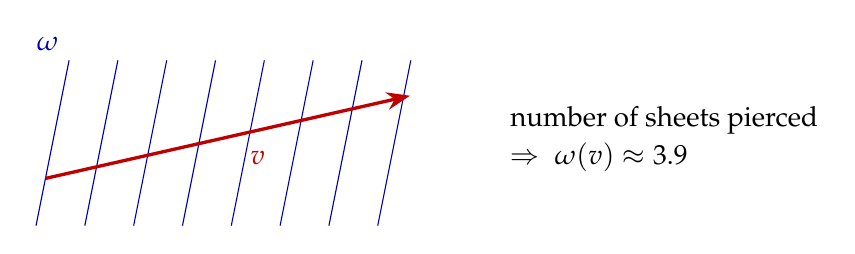
\begin{tikzpicture}[>=Stealth]
  \foreach \i in {0,...,7}{\draw[blue!65!black,thin] (\i*0.62,-0.45)--(\i*0.62+0.42,1.65);}
  \draw[->,red!75!black,very thick] (0.12,0.15)--(4.75,1.20);
  \node[red!75!black,below right] at (2.6,0.62) {$v$};
  \node[blue!65!black,above] at (0.15,1.65) {$\omega$};
  \node[align=left,anchor=west] at (5.9,0.65) {number of sheets pierced\\[2pt] $\Rightarrow\ \omega(v)\approx 3.9$};
\end{tikzpicture}
\caption{Geometric picture of contraction. A covector $\omega$ is a ``stack of parallel sheets'' (its level sets); the vector
$v$ is an arrow; $\omega(v)$ counts how many sheets the arrow pierces. Doubling $v$ doubles the count, and reversing $v$
changes the sign: this is linearity.}
\label{fig:sheets}
\end{figure}

\begin{keyidea}
\textbf{Contraction is the metric-free pairing $V^*\times V\to\R$.} Everything later that looks like a ``dot product'' in physics
-- work $\mathbf F\cdot\dd\mathbf r$, power, flux, the pairing of a momentum with a symmetry -- is, when examined, a contraction
$\langle\omega,v\rangle$ of a covector with a vector. A metric is needed only when one wants to turn an arrow into a ruler or
vice versa (Section~\ref{sec:metric}).
\end{keyidea}

Contraction is the first member of a family: it extends to tensors of any type (Section~\ref{sec:tensors}), to
$k$-forms as the \emph{interior product} $\iota_v\alpha$ (Section~\ref{sec:interior}), and to multivectors as the
\emph{left contraction} $a\lc A$ of geometric algebra (Section~\ref{sec:ops}); Section~\ref{sec:synth1} compares these four
guises. On a manifold the same pairing is performed at every point between the cotangent space and the tangent space
(Section~\ref{sec:tangent}), and integrating along a curve will turn out to be nothing more than contracting a $1$-form with the
velocity (Section~\ref{sec:int1}).


% =====================================================================
\section{Multilinear maps, tensors and the tensor algebra}\label{sec:tensors}
% =====================================================================

Contraction pairs one covector with one vector. To measure with several covectors at once, and to build
bilinear objects such as a metric or a curvature, we need multilinear maps and their algebra. This section gives the
concrete (``machine'') description of tensors, the abstract description by a universal property, and the tensor algebra,
the free algebra from which every algebra of Part~\ref{part:algebra} is obtained by imposing relations.

\subsection{Multilinear maps}\label{sec:multilinear}
% ---- begin extract GR lines 207-217 ----
\begin{formal}[{multilinear map}]
Let $E_1,\dots,E_k$ be vector spaces. A map $f:E_1\times\dots\times E_k\to\R$ is \emph{multilinear} if it is linear in each slot when the other slots are held fixed:
\[
f(v_1,\dots,u+t\tilde u,\dots,v_k)=f(v_1,\dots,u,\dots,v_k)+t\,f(v_1,\dots,\tilde u,\dots,v_k).
\]
Examples: a linear form ($k=1$) is an element of $E^*$; the dot product $\langle v_1,v_2\rangle$ is bilinear ($k=2$); the determinant of $m$ column vectors is $m$-linear.
\end{formal}

\begin{intuition}[{linear in every slot = ``a machine with several input slots''}]
A multilinear map is a machine with $k$ input hoppers. You may feed any vector in each hopper; the output is a number that depends linearly on what is in each hopper \emph{separately}. Multilinear maps are exactly the maps that are completely determined by their values on basis vectors.
\end{intuition}
%% ---- end extract ----

% ---- begin extract GA lines 155-170 ----
\begin{definition}[Multilinear map]
Let $V_1,\dots,V_k,U$ be vector spaces. A map $\beta:V_1\times\cdots\times V_k\to U$ is
\emph{multilinear} if it is linear in each argument when the others are held fixed.
For $k=2$ we say \emph{bilinear}. If all $V_i=V$ and
$\beta(\dots,v_i,\dots,v_j,\dots)=-\beta(\dots,v_j,\dots,v_i,\dots)$ for all $i\neq j$,
$\beta$ is \emph{alternating}; we write $\Alt^k(V;U)$ for the space of such maps.
\end{definition}

\begin{example}
The determinant $\det:(\K^n)^n\to\K$ (as a function of the $n$ columns) is multilinear and alternating.
The dot product $\R^n\times\R^n\to\R$ is bilinear (and symmetric).
\end{example}

The crucial remark is that a bilinear map is \emph{not} a linear map on $V\times W$:
$\beta(2u,2w)=4\beta(u,w)$, whereas a linear map would give $2\beta(u,w)$. The tensor product
will fix exactly this defect.
%% ---- end extract ----


\subsection{The tensor product}\label{sec:tensorproduct}
% ---- begin extract GR lines 220-238 ----
\begin{formal}[{tensor product of multilinear maps}]
Given multilinear $f:E_1\times\dots\times E_k\to\R$ and $g:F_1\times\dots\times F_\ell\to\R$, their \emph{tensor product} is the multilinear map $f\otimes g:E_1\times\dots\times E_k\times F_1\times\dots\times F_\ell\to\R$,
\[
(f\otimes g)(v_1,\dots,v_k,u_1,\dots,u_\ell)=f(v_1,\dots,v_k)\cdot g(u_1,\dots,u_\ell).
\]
Properties: bilinear and associative, but \textbf{not commutative} in general ($f\otimes g\ne g\otimes f$). If $\{e^{i}\}$ is the dual basis of $E_1$ and $\{f^{j}\}$ that of $E_2$, then $\{e^{i}\otimes f^{j}\}$ is a basis of the space of bilinear maps $E_1\times E_2\to\R$, which is written $E_1^*\otimes E_2^*$; its dimension is $\dim E_1\cdot\dim E_2$.
\end{formal}

\begin{intuition}[{``run both machines side by side and multiply the outputs''}]
$f\otimes g$ is a machine with the hoppers of $f$ followed by the hoppers of $g$. It feeds the first group to $f$, the second group to $g$, and multiplies the two numbers. It is the most ``free'' way to combine two machines: all other bilinear machines are built by \emph{adding} such products. Not every bilinear machine is a single product: $e^{1}\otimes e^{2}+e^{2}\otimes e^{1}$ cannot be written as $f\otimes g$ (it is the symmetric ``product'' used for metrics).
\end{intuition}

\begin{example}[{tensor product of two covectors on $\R^2$}]
Take $f=e^{1}+2e^{2}$, $g=3e^{1}-e^{2}$. Then
\[
f\otimes g=3\,e^{1}\!\otimes e^{1}-e^{1}\!\otimes e^{2}+6\,e^{2}\!\otimes e^{1}-2\,e^{2}\!\otimes e^{2},
\]
and $(f\otimes g)(v,w)=(v^1+2v^2)(3w^1-w^2)$. Its component matrix $(f_ig_j)=\begin{pmatrix}3&-1\\6&-2\end{pmatrix}$ has rank 1. Contrast $g\otimes f$: components $(g_if_j)=\begin{pmatrix}3&6\\-1&-2\end{pmatrix}$, the transpose.
\end{example}
%% ---- end extract ----


\subhead{The abstract definition: a universal property}
The functional definition above is convenient for computing. The following characterisation does not depend on any
construction and is the one used to define the algebras of the next sections.
% ---- begin extract GA lines 202-231 ----

\begin{definition}[Tensor product]\label{def:tensor}
Let $V,W$ be vector spaces. A \emph{tensor product} of $V$ and $W$ is a vector space
$V\otimes W$ together with a bilinear map $\otimes:V\times W\to V\otimes W$,
$(v,w)\mapsto v\otimes w$, such that the following \emph{universal property} holds:
for every vector space $U$ and every bilinear map $\beta:V\times W\to U$ there exists a
\emph{unique linear} map $\tilde\beta:V\otimes W\to U$ with $\beta=\tilde\beta\circ\otimes$.
\[
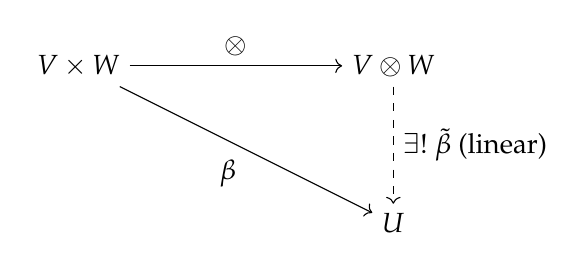
\begin{tikzpicture}[baseline=(current bounding box.center)]
  \node (VW) at (0,0) {$V\times W$};
  \node (T)  at (4,0) {$V\otimes W$};
  \node (U)  at (4,-2) {$U$};
  \draw[->] (VW) -- node[above]{$\otimes$} (T);
  \draw[->] (VW) -- node[below left]{$\beta$} (U);
  \draw[->,dashed] (T) -- node[right]{$\exists!\ \tilde\beta$ (linear)} (U);
\end{tikzpicture}
\]
\end{definition}

In words: \emph{bilinear maps out of $V\times W$ are the same thing as linear maps out of $V\otimes W$}.

\begin{proposition}[Uniqueness]
If $(T_1,\otimes_1)$ and $(T_2,\otimes_2)$ both satisfy Definition~\ref{def:tensor}, there is a unique
linear isomorphism $\phi:T_1\to T_2$ with $\phi(v\otimes_1w)=v\otimes_2w$.
\end{proposition}
\begin{proof}
Apply the universal property of $T_1$ to $\otimes_2$ to get $\phi:T_1\to T_2$, and that of $T_2$ to $\otimes_1$ to get
$\psi:T_2\to T_1$. Then $\psi\circ\phi$ is a linear map $T_1\to T_1$ compatible with $\otimes_1$, as is $\id_{T_1}$;
by the uniqueness clause they coincide. Likewise $\phi\circ\psi=\id_{T_2}$.
\end{proof}
%% ---- end extract ----

% ---- begin extract GA lines 234-277 ----

Let $F(V\times W)$ be the \emph{free vector space} on the \emph{set} $V\times W$: formal finite linear combinations
$\sum_a c_a\,[(v_a,w_a)]$ of the symbols $[(v,w)]$, which are declared linearly independent.
Let $N\subset F(V\times W)$ be the subspace spanned by all elements of the form
\begin{align*}
&[(v+v',w)]-[(v,w)]-[(v',w)], & &[(v,w+w')]-[(v,w)]-[(v,w')],\\
&[(\lambda v,w)]-\lambda[(v,w)], & &[(v,\lambda w)]-\lambda[(v,w)].
\end{align*}
Define $V\otimes W:=F(V\times W)/N$ and $v\otimes w:=[(v,w)]+N$. By construction $\otimes$ is bilinear.
Given a bilinear $\beta$, the linear extension of $[(v,w)]\mapsto\beta(v,w)$ to the free space kills $N$,
hence descends to the unique $\tilde\beta$ required. 

\begin{theorem}[Basis and dimension]\label{thm:tensorbasis}
If $(e_i)_{i\le n}$ and $(f_j)_{j\le m}$ are bases of $V$ and $W$, then $(e_i\otimes f_j)$ is a basis of $V\otimes W$.
In particular $\dim(V\otimes W)=nm$.
\end{theorem}
\begin{proof}[Proof sketch]
\emph{Spanning:} by bilinearity, $(v^ie_i)\otimes(w^jf_j)=v^iw^j\,e_i\otimes f_j$, and elements $v\otimes w$ span $V\otimes W$ by construction.
\emph{Independence:} for each pair $(k,l)$ the map $\beta_{kl}(v,w)=e^k(v)f^l(w)$ is bilinear, so it induces a linear
functional $\tilde\beta_{kl}$ on $V\otimes W$ with $\tilde\beta_{kl}(e_i\otimes f_j)=\delta_{ik}\delta_{jl}$. If $\sum c^{ij}e_i\otimes f_j=0$,
applying $\tilde\beta_{kl}$ gives $c^{kl}=0$.
\end{proof}

A general element is therefore $T=T^{ij}\,e_i\otimes f_j$. Elements of the form $v\otimes w$ are called
\emph{pure} (or decomposable); they are the exception rather than the rule: $e_1\otimes e_2+e_2\otimes e_1$ is not pure
(its coefficient matrix has rank $2$; pure tensors are exactly the rank-$1$ matrices).

\begin{proposition}[Standard identifications (finite dimension)]
\begin{enumerate}
  \item $V\otimes\K\cong V$ and $(U\otimes V)\otimes W\cong U\otimes(V\otimes W)$ (associativity).
  \item $V^*\otimes W\cong\Hom(V,W)$ via $(\varphi\otimes w)(v)=\varphi(v)\,w$. In coordinates, $T^{i}{}_{j}\,e_i\otimes e^j$ is a matrix.
  \item $(V\otimes W)^*\cong V^*\otimes W^*$, and $V^*\otimes V^*\cong\{\text{bilinear forms on }V\}$. Hence a metric $g=g_{ij}e^i\otimes e^j$ is a tensor in $V^*\otimes V^*$.
\end{enumerate}
\end{proposition}

\begin{intuition}
The symbol $v\otimes w$ is a ``\emph{formal product that remembers nothing except bilinearity}''. You may
pull scalars out and distribute over sums, but you may \emph{not} simplify further: $v\otimes w\neq w\otimes v$,
and $v\otimes w$ is not a number or a vector, it is a new kind of object.
A concrete picture: $v\otimes w$ is the rank-one matrix $vw^{\mathsf T}$ (a table whose $(i,j)$ entry is $v^iw^j$);
a general tensor is a sum of such tables, i.e.\ any $n\times m$ table. The tensor product is thus the
\emph{space of all tables}, and the universal property says that any bilinear recipe can be evaluated by first
building the table and then applying a linear map to it.
\end{intuition}
%% ---- end extract ----


\subsection{Tensors of type $(\ell,k)$}\label{sec:tensortypes}
% ---- begin extract GR lines 241-286 ----
\begin{formal}[{tensors}]
A \emph{mixed tensor, $k$-covariant and $\ell$-contravariant} on $E$ is a multilinear map
\[
\tau:\underbrace{E\times\dots\times E}_{k}\times\underbrace{E^*\times\dots\times E^*}_{\ell}\to\R .
\]
The space of such tensors is $\TT{\ell}{k}(E)\cong \underbrace{E^*\otimes\dots\otimes E^*}_{k}\otimes\underbrace{E\otimes\dots\otimes E}_{\ell}$. Conventionally $\TT{0}{0}(E)=\R$ (scalars). Special cases:
\begin{center}
\begin{tabular}{@{}lll@{}}
\toprule
Space & Meaning & Components\\ \midrule
$\TT{0}{0}=\R$ & scalar & $\tau$\\
$\TT{0}{1}=E^*$ & covector & $f_i$\\
$\TT{1}{0}=(E^*)^*\cong E$ & vector & $v^i$\\
$\TT{0}{2}$ & bilinear form (\eg metric) & $g_{ij}$\\
$\TT{1}{1}$ & linear map $E\to E$ (via $A(v,\alpha)=\alpha(Av)$) & $A^i{}_j$\\
$\TT{1}{2}$ & (\eg torsion) & $T^i{}_{jk}$\\
$\TT{1}{3}$ & (\eg Riemann curvature) & $R^l{}_{ijk}$\\ \bottomrule
\end{tabular}
\end{center}
\end{formal}

\begin{intuition}[{a tensor is a coordinate-free machine; its components are a table}]
A tensor is a geometric object like a vector: it exists independently of any basis. It is a machine with $k$ ``vector hoppers'' and $\ell$ ``covector hoppers'' that returns a number. The components are just the table of outputs on basis elements:
\[
\tau^{i_1\dots i_\ell}{}_{j_1\dots j_k}=\tau\big(e_{j_1},\dots,e_{j_k},e^{i_1},\dots,e^{i_\ell}\big).
\]
So $\tau=\tau^{i_1\dots i_\ell}{}_{j_1\dots j_k}\;e^{j_1}\otimes\dots\otimes e^{j_k}\otimes e_{i_1}\otimes\dots\otimes e_{i_\ell}$.
\end{intuition}

\begin{formal}[{transformation rule of components}]
If $e'_i=A^j{}_ie_j$, the components of a tensor in the new basis are
\begin{equation}\label{eq:tensortransf}
\tau'^{\,i_1\dots i_\ell}{}_{j_1\dots j_k}=(A^{-1})^{i_1}{}_{a_1}\cdots(A^{-1})^{i_\ell}{}_{a_\ell}\;A^{b_1}{}_{j_1}\cdots A^{b_k}{}_{j_k}\;\tau^{a_1\dots a_\ell}{}_{b_1\dots b_k}.
\end{equation}
Each upper index is transformed with $A^{-1}$, each lower index with $A$. A physicist's definition: \emph{a tensor is an array of numbers that transforms like this under changes of basis}. (In the notes this appears with $B=A$.)
\end{formal}

\begin{example}[{three ``matrices'', three different transformation laws}]
In matrix notation, with $M$ the component matrix and $A$ the change of basis:
\[
\TT{0}{2}\ (g_{ij}):\ M'=A^tMA,\qquad
\TT{1}{1}\ (A^i{}_j):\ M'=A^{-1}MA,\qquad
\TT{2}{0}\ (T^{ij}):\ M'=A^{-1}M A^{-t}.
\]
\emph{Test.} Dot product on $\R^2$, $g=\mathrm{diag}(1,1)$, and $A=\begin{pmatrix}1&-1\\1&1\end{pmatrix}$ from Section~\ref{sec:vs}: $g'=A^tA=\begin{pmatrix}2&0\\0&2\end{pmatrix}$: the new basis vectors are still orthogonal but have length $\sqrt2$. \emph{Test 2.} The trace of a $(1,1)$ tensor is invariant, $\tr(A^{-1}MA)=\tr M$, but $\tr(A^tMA)\neq\tr M$ in general: ``trace of a bilinear form'' is not a meaningful invariant without a metric.
\end{example}
%% ---- end extract ----


\subsection{Symmetric and antisymmetric tensors; contraction of tensors}\label{sec:symcontr}
% ---- begin extract GR lines 289-312 ----
A tensor $\tau\in\TT{0}{2}$ is \emph{symmetric} if $\tau(v,w)=\tau(w,v)$ and \emph{antisymmetric} if $\tau(v,w)=-\tau(w,v)$. For covectors $\alpha,\beta$ we define the \emph{wedge product}
\[
\alpha\wedge\beta=\alpha\otimes\beta-\beta\otimes\alpha.
\]
The notes use this in the area-form of the sphere: $r^2\sin\theta\,\dd\theta\wedge\dd\varphi$. Intuitively, $\alpha\wedge\beta(v,w)=\alpha(v)\beta(w)-\alpha(w)\beta(v)$ is the signed area of the parallelogram spanned by $v,w$ as seen through the ``rulers'' $\alpha,\beta$.

\subhead{Contraction}
\begin{formal}[{contraction}]
The evaluation $E\times E^*\to\R$, $(v,f)\mapsto f(v)$ is bilinear, with $e_i,e^{j}\mapsto\delta^j{}_i$. Applying it to one covariant and one contravariant slot of a tensor gives a new tensor of type $(\ell-1,k-1)$. In components: set an upper and a lower index equal and sum,
\[
(c\tau)^{i_2\dots}{}_{j_2\dots}=\tau^{s\,i_2\dots}{}_{s\,j_2\dots}.
\]
\end{formal}
\begin{intuition}[{contraction = plug a vector-slot into a covector-slot}]
Think of connecting an output cable of one slot to the input of another and ``summing over all possible signals''. The result is lower in rank and \emph{still a tensor}. Examples: the trace $A^i{}_i$ of a linear map; the pairing $f_iv^i$; later the Ricci tensor $R^i{}_{ijk}$ and the scalar curvature.
\end{intuition}

\begin{exercises}
\begin{enumerate}[nosep]
\item Show that $\dim\TT{\ell}{k}(E)=m^{k+\ell}$.
\item For $E=\R^3$, $e'_1=2e_1$, $e'_2=e_2$, $e'_3=e_3+e_1$: compute the dual basis change, and the components of $f=e^{1}+e^{3}$ in the new basis.
\item Show that the identity map of $E$ is the $(1,1)$ tensor $\delta^i{}_j$ with the same components in every basis.
\end{enumerate}
\end{exercises}
%% ---- end extract ----


\begin{remark}[Three kinds of $2$-tensors]
A tensor in $\TT{0}{2}$ may be symmetric, antisymmetric, or neither; every one splits uniquely into a symmetric and an
antisymmetric part. A \emph{metric} is symmetric and non-degenerate (Section~\ref{sec:metric}); a \emph{$2$-form} is
antisymmetric (Section~\ref{sec:ext}); a general bilinear form such as $\dd x\otimes\dd y$ has both parts. The two parts
do different jobs -- one measures length, the other oriented area -- and the symmetric/antisymmetric bookkeeping
is made precise in Section~\ref{sec:wedgetensor}.
\end{remark}

\subsection{The tensor algebra, and ``choose your relations''}\label{sec:tensoralgebra}
% ---- begin extract GA lines 281-311 ----
Write $V^{\otimes 0}=\K$, $V^{\otimes k}=V\otimes\cdots\otimes V$ ($k$ factors), of dimension $n^k$.

\begin{definition}[Tensor algebra]
$T(V)=\bigoplus_{k\ge0}V^{\otimes k}$, with the associative bilinear product induced by concatenation:
\[
 (v_1\otimes\cdots\otimes v_k)\cdot(w_1\otimes\cdots\otimes w_l)=v_1\otimes\cdots\otimes v_k\otimes w_1\otimes\cdots\otimes w_l .
\]
The unit is $1\in V^{\otimes0}=\K$. It is a \emph{graded algebra}: $V^{\otimes k}\cdot V^{\otimes l}\subset V^{\otimes(k+l)}$.
\end{definition}

\begin{theorem}[Universal property of $T(V)$]\label{thm:Tuniv}
For every unital associative algebra $A$ and every linear map $f:V\to A$ there is a unique algebra homomorphism
$\bar f:T(V)\to A$ with $\bar f|_V=f$, namely $\bar f(v_1\otimes\cdots\otimes v_k)=f(v_1)f(v_2)\cdots f(v_k)$.
\end{theorem}

This says $T(V)$ is the \emph{free} associative algebra generated by $V$: no relations are imposed on products.
Consequently every algebra generated by $V$ is a quotient $T(V)/\mathcal I$ for a two-sided ideal $\mathcal I$ of relations.

\begin{intuition}
Think of $T(V)$ as ``words'' in the ``alphabet'' $V$: $e_1e_2e_1$ and $e_1e_1e_2$ are different words.
Imposing a relation such as ``$vv=0$'' or ``$vv=|v|^2$'' is like declaring certain words equivalent and so
collapsing the (enormous) free algebra to a smaller one. Different relations give different geometries:
\begin{center}
\begin{tabular}{lll}
relation on $v\in V$ & resulting algebra & geometric content\\\hline
$v\otimes w=w\otimes v$ & symmetric algebra $S(V)$ & polynomials\\
$v\otimes v=0$ & exterior algebra $\bigwedge V$ & oriented areas, volumes\\
$v\otimes v=Q(v)$ & Clifford algebra $\Cl(V,Q)$ & lengths, angles, areas, rotations
\end{tabular}
\end{center}
\end{intuition}
%% ---- end extract ----


% =====================================================================
\section{The metric tensor and the musical isomorphisms}\label{sec:metric}
% =====================================================================

The dual space $V^*$ exists with no further structure. A \emph{metric} is extra structure: a symmetric non-degenerate
$2$-tensor. It is the only thing that allows us to speak of lengths and angles, and it provides the dictionary
between vectors and covectors (the ``musical isomorphisms'' $\flat$ and $\sharp$). Remember the division of labour
that runs through the document: \emph{covectors, forms and contraction need no metric; gradients, curl, Hodge star and the geometric
product do.}
% ---- begin extract GR lines 317-369 ----
\begin{formal}[{metric}]
A \emph{metric} on $E$ is a tensor $g\in\TT{0}{2}(E)$ (a bilinear map $g:E\times E\to\R$) such that
\begin{enumerate}[label=(\roman*),nosep]
\item $g(v,w)=g(w,v)$ (symmetric);
\item $g(v,w)=0\ \ \forall w\in E\ \Rightarrow\ v=0$ (non-degenerate).
\end{enumerate}
In a basis, $g=g_{ij}\,e^{i}\otimes e^{j}$ with $(g_{ij})$ a symmetric \emph{invertible} matrix. Being symmetric, it can be diagonalized over $\R$; if it has $p$ positive and $q$ negative eigenvalues, the \emph{signature} is $\sig(g)=(p,q)$ (it does not depend on the basis, by Sylvester's law of inertia). 
\begin{itemize}[nosep]
\item $\sig=(m,0)$ (positive definite): \textbf{Riemannian}: $g$ is an inner product.
\item $\sig=(m-1,1)$: \textbf{Lorentzian} (one negative direction, ``mostly plus''), used in GR with $m=4$, $\sig(g)=(3,1)$, \eg Minkowski $\eta=\mathrm{diag}(-1,1,1,1)$. The opposite sign convention (``mostly minus'', $\eta=\mathrm{diag}(1,-1,-1,-1)$, signature $(1,3)$) is used in the spacetime algebra of Section~\ref{sec:clifford}.
\end{itemize}
The \emph{norm squared} is $\|v\|^2=g(v,v)$, which can be positive, zero or negative in the Lorentzian case.
\end{formal}

\begin{intuition}[{the metric is the ``dot product'': it defines lengths, angles and (in GR) causality}]
$g(v,w)$ tells you the length of $v$, the angle between $v$ and $w$, and the projection of $v$ on $w$. In ordinary space all vectors have $g(v,v)\geq0$. In relativity the metric is \emph{indefinite}: a vector $v$ with $g(v,v)<0$ is \textbf{timelike} (a possible velocity of a massive particle), $g(v,v)=0$ with $v\ne0$ is \textbf{null} (light), $g(v,v)>0$ is \textbf{spacelike}. The null vectors form the \emph{light cone} and non-degeneracy does not mean ``$g(v,v)\neq0$ for all $v\neq0$'', it only means that $v\neq0$ always has \emph{some} partner $w$ with $g(v,w)\neq0$.
\end{intuition}

\begin{formal}[{musical isomorphisms (raising and lowering indices)}]
A metric gives an isomorphism between $E$ and $E^*$:
\[
g^\flat:E\to E^*,\quad v\mapsto g(v,\cdot),\qquad\qquad g^\sharp:=(g^\flat)^{-1}:E^*\to E.
\]
In components: $(g^\flat v)_k=v^jg_{jk}=:v_k$ (``lowering the index''), and, with $(g^{kl})$ the inverse matrix of $(g_{ij})$ (so $g^{ij}g_{jk}=\delta^i{}_k$), $(g^\sharp f)^l=f_kg^{kl}=:f^l$ (``raising the index''). The \emph{inverse metric} $g^{-1}=g^{ij}e_i\otimes e_j\in\TT{2}{0}$ is the induced metric on $E^*$. More generally the metric lets us raise or lower any index of any tensor, \eg $T^i{}_j\mapsto T_{ij}=g_{ik}T^k{}_j$; contraction with $g^{ij}$ is the way to take traces of $(0,2)$ tensors.
\end{formal}

\begin{intuition}[{the metric identifies arrows with rulers}]
Given an arrow $v$, the covector $g(v,\cdot)$ is ``the ruler that measures how much of any vector $w$ lies along $v$ (scaled by $|v|$)''. This is the \emph{only} reason why in Euclidean space we can pretend that arrows and covectors are the same thing: with $g=\delta_{ij}$ lowering and raising indices does not change the numbers. With another metric (polar coordinates, curved space, Minkowski) the numbers do change, and the difference between upper and lower indices matters.
\end{intuition}

\begin{example}[{Minkowski space}]
$\eta=\mathrm{diag}(-1,1,1,1)$, $\eta^{-1}=\mathrm{diag}(-1,1,1,1)$ too. For $v=(v^0,v^1,v^2,v^3)$ the lowered components are $v_\mu=(-v^0,v^1,v^2,v^3)$, so
\[
\eta(v,v)=-(v^0)^2+(v^1)^2+(v^2)^2+(v^3)^2.
\]
The vector $(1,1,0,0)$ is null (a light ray with $c=1$), $(2,1,0,0)$ is timelike, $(1,2,0,0)$ is spacelike. For a worldline $x^\mu(\tau)$, \emph{proper time} is $\dd\tau^2=-\eta(\dot x,\dot x)\,\dd\lambda^2$. A Lorentz transformation is precisely a basis change $A$ with $A^t\eta A=\eta$ (compare with $M'=A^tMA$ in Section~\ref{sec:tensors}).
\end{example}

\begin{example}[{raising an index in polar coordinates: the gradient}]
In $\R^2$ with polar coordinates $(r,\varphi)$ (see Example~\ref{ex:polarmetric} below for the derivation) the metric components are $g=\mathrm{diag}(1,r^2)$, $g^{-1}=\mathrm{diag}(1,r^{-2})$. The covector $\dd f=\partial_rf\,\dd r+\partial_\varphi f\,\dd\varphi$ becomes, after raising the index, the vector
\[
\nabla f=g^\sharp(\dd f)=\partial_rf\;\partial_r+\frac{1}{r^2}\partial_\varphi f\;\partial_\varphi .
\]
The familiar $\frac1r\partial_\varphi f\,\hat e_\varphi$ is the same thing written in the \emph{unit} basis $\hat e_\varphi=\frac1r\partial_\varphi$.
\end{example}

\begin{exercises}
\begin{enumerate}[nosep]
\item Show that if $g(v,v)>0$ for all $v\neq0$, then $g$ is non-degenerate. Give a symmetric bilinear form on $\R^2$ that is degenerate.
\item In Minkowski space, find $w$ with $\eta(w,w)=0$, $w\ne0$ and $\eta(w,u)\neq0$ for some $u$. Why is this consistent with non-degeneracy?
\item Compute $g^\flat$ of $v=\partial_\varphi$ in polar coordinates.
\end{enumerate}
\end{exercises}
%% ---- end extract ----


\subsection{Quadratic forms, polarization and signature}\label{sec:quadform}
The geometric algebra of Sections~\ref{sec:clifford}--\ref{sec:duality} is built directly on the quadratic form $Q(v)=g(v,v)$
associated with the metric, so we recall the relation between the two and the notation for the signature.
% ---- begin extract GA lines 174-195 ----
\begin{definition}[Metric, quadratic form]
A \emph{metric} on $V$ is a symmetric bilinear form $g:V\times V\to\K$. It induces the
\emph{quadratic form} $Q(v)=g(v,v)$, and conversely (when $\mathrm{char}\,\K\neq2$) $g$ is
recovered by \emph{polarization}:
\begin{equation}\label{eq:polar}
  g(u,v)=\tfrac12\bigl(Q(u+v)-Q(u)-Q(v)\bigr).
\end{equation}
$g$ is \emph{non-degenerate} if $g(u,\cdot)=0$ implies $u=0$. By Sylvester's law of inertia, over
$\R$ there is an \emph{orthonormal basis} with $g(e_i,e_j)=0$ for $i\neq j$ and
$g(e_i,e_i)\in\{+1,-1,0\}$; the numbers $(p,q,r)$ of $+1,-1,0$ form the \emph{signature}.
We write $\R^{p,q}$ when $r=0$ and $\R^n=\R^{n,0}$ for the Euclidean case.
\end{definition}

A non-degenerate metric yields the \emph{musical isomorphism} $\flat:V\to V^*$,
$v\mapsto g(v,\cdot)$, which allows us to identify vectors and covectors.
We shall write $u\cdot v:=g(u,v)$.

\begin{intuition}
The metric is the ruler-and-protractor: it tells you how long vectors are and what angle they make.
Signature $(p,q)$ says that $p$ directions behave like space and $q$ like time (e.g.\ $\R^{1,3}$ for
special relativity). The exterior algebra will need \emph{no} metric; geometric algebra needs one.
\end{intuition}
%% ---- end extract ----


\begin{pitfall}[three sign conventions for the signature]
(i) Throughout this document the signature $(p,q)$ counts $p$ \emph{positive} and $q$ \emph{negative} eigenvalues,
so that $\R^{p,q}$ and $\Cl(p,q)$ have $p$ basis vectors with $e_i^2=+1$ and $q$ with $e_i^2=-1$; Euclidean space is $(n,0)$.
(ii) General relativity (and Sections~\ref{sec:phys}--\ref{sec:bridge}) uses ``mostly plus'' $\eta=\mathrm{diag}(-1,1,1,1)$, i.e.\ signature
$(3,1)$; (iii) the spacetime algebra of Section~\ref{sec:ga-calculus} uses ``mostly minus'' $\gamma_0^2=+1$, $\gamma_i^2=-1$, i.e.\ $(1,3)$.
Physical statements are the same in the two conventions; only the signs of formulas such as $\vd^2=\pm\Box$ or
$p^2=\mp m^2$ differ. Always check which one a formula assumes.
\end{pitfall}

\begin{keypoints}[vectors, tensors and the metric]
\begin{itemize}
\item Vectors have components that transform \emph{against} the basis; covector components transform \emph{with} it; their contraction $\omega_iv^i$ is invariant and metric-free.
\item A tensor of type $(\ell,k)$ is a multilinear machine; $T(V)$ is the free algebra on $V$ and every later algebra is $T(V)$ modulo relations.
\item A metric converts vectors into covectors ($\flat$) and back ($\sharp$); without it there is no ``gradient vector'' and no angle.
\end{itemize}
\end{keypoints}


% =====================================================================
\section{The exterior algebra and the wedge product}\label{sec:ext}
% =====================================================================

The wedge product $\dd x\wedge\dd y$ is used freely from here on. This section says exactly what the exterior (wedge) product
is, which rules it obeys, and how it sits inside the tensor product. It is presented in two equivalent ways that the literature
alternates between: \emph{(a)} forms as alternating multilinear maps on $V$, i.e.\ elements of $\bigwedge^kV^*$, with an explicit
formula for $\wedge$ (Sections~\ref{sec:altforms}--\ref{sec:wedgeprops}); and \emph{(b)} the exterior algebra
$\bigwedge V=T(V)/\langle v\otimes v\rangle$ as a quotient, whose elements are \emph{multivectors}
(Sections~\ref{sec:extquotient}--\ref{sec:blades}). They are identified in Remark~\ref{rem:twomodels}. Throughout, $V$ is a real
vector space of dimension $n$ (think $V=T_pM$ with basis $\partial_i$ and dual basis $\dd x^i$).

\subsection{Alternating forms and the wedge product}\label{sec:altforms}

\begin{definition}[Alternating forms]
A \emph{$k$-form} on $V$ is a map $\alpha:V\times\cdots\times V\to\R$ ($k$ arguments) that is linear in each argument and
\emph{alternating}: exchanging two arguments changes the sign,
$\alpha(\dots,v,\dots,w,\dots)=-\alpha(\dots,w,\dots,v,\dots)$. In particular $\alpha$ vanishes if two arguments are equal,
or more generally linearly dependent. The space of $k$-forms is denoted $\bigwedge^kV^*$ ($=\Alt^k(V;\R)$); $\bigwedge^0V^*=\R$ and
$\bigwedge^1V^*=V^*$.
\end{definition}

\begin{definition}[Wedge product]
For $\alpha\in\bigwedge^kV^*$ and $\beta\in\bigwedge^lV^*$,
\begin{equation}\label{eq:wedge}
(\alpha\wedge\beta)(v_1,\dots,v_{k+l})=\frac1{k!\,l!}\sum_{\sigma\in S_{k+l}}\sgn(\sigma)\;
\alpha\bigl(v_{\sigma(1)},\dots,v_{\sigma(k)}\bigr)\,\beta\bigl(v_{\sigma(k+1)},\dots,v_{\sigma(k+l)}\bigr),
\end{equation}
where $S_{k+l}$ is the group of permutations of $k+l$ objects. The result is a $(k+l)$-form.
\end{definition}

\begin{specialcase}[$k=l=1$: the case that matters most]
The sum has two terms, $\sigma=\id$ and the exchange of $1$ and $2$, and the prefactor is $1$:
\begin{equation}\label{eq:wedge11}
(\alpha\wedge\beta)(v,w)=\alpha(v)\beta(w)-\alpha(w)\beta(v).
\end{equation}
For $\alpha=\dd x$, $\beta=\dd y$ this is $(\dd x\wedge\dd y)(a,b)=a^xb^y-a^yb^x$, the determinant of the projections of
$a,b$ onto the $xy$-plane.
\end{specialcase}

\begin{proposition}[Determinant formula]\label{prop:detformula}
For $1$-forms $\alpha^1,\dots,\alpha^k$ and vectors $v_1,\dots,v_k$,
\begin{equation}\label{eq:detformula}
(\alpha^1\wedge\cdots\wedge\alpha^k)(v_1,\dots,v_k)=\det\bigl[\alpha^i(v_j)\bigr]_{i,j=1}^k .
\end{equation}
\end{proposition}
\begin{proof}
Apply \eqref{eq:wedge} repeatedly. The normalisation $1/(k!\,l!)$ exactly compensates the repetitions in the sum over
permutations, so an iterated wedge of $1$-forms is the single sum $\sum_\sigma\sgn(\sigma)\alpha^1(v_{\sigma(1)})\cdots\alpha^k(v_{\sigma(k)})$,
which is the Leibniz expansion of the determinant.
\end{proof}

\begin{intuition}[geometric meaning of the determinant formula]
The matrix $[\alpha^i(v_j)]$ is the matrix of the vectors $v_j$ after they have been mapped by
$A:V\to\R^k$, $A(v)=(\alpha^1(v),\dots,\alpha^k(v))$. So \eqref{eq:detformula} is the signed $k$-dimensional volume of the image
of the parallelepiped $(v_1,\dots,v_k)$ under $A$. For $\dd x\wedge\dd y$ in $\R^3$: the signed area of the \emph{projection} of
the parallelogram $(v,w)$ onto the $xy$-plane. (In the picture of Figure~\ref{fig:sheets}: the stacks of sheets of $\alpha$ and
$\beta$ intersect in a honeycomb of tubes, and $(\alpha\wedge\beta)(v,w)$ counts the tubes pierced by the parallelogram.)
The sign records the orientation; it is the reason why forms, and not arbitrary tensors, are the integrands of oriented surfaces
(Section~\ref{sec:intk}).
\end{intuition}

\begin{example}[Projected areas are the components of the cross product]\label{ex:projareas}
In $\R^3$ take $v=(1,0,2)$ and $w=(0,1,5)$. Evaluate the three coordinate $2$-forms with \eqref{eq:wedge11}:
\begin{align*}
(\dd y\wedge\dd z)(v,w)&=v^yw^z-v^zw^y=0\cdot5-2\cdot1=-2,\\
(\dd z\wedge\dd x)(v,w)&=v^zw^x-v^xw^z=2\cdot0-1\cdot5=-5,\\
(\dd x\wedge\dd y)(v,w)&=v^xw^y-v^yw^x=1\cdot1-0\cdot0=1.
\end{align*}
These are exactly the components of $v\times w=(-2,-5,1)$: the cross product lists the areas of the three projections of the
parallelogram. Note that the third value ignores the $z$-components $2$ and $5$, as a projection must
(Sections~\ref{sec:phys-cross}, \ref{sec:duality}).
\end{example}

\begin{proposition}[Basis and dimension]\label{prop:formbasis}
For increasing multi-indices $I=(i_1<\cdots<i_k)$ put $\dd x^I=\dd x^{i_1}\wedge\cdots\wedge\dd x^{i_k}$. Every $k$-form is uniquely
\[
\alpha=\sum_{i_1<\cdots<i_k}\alpha(\partial_{i_1},\dots,\partial_{i_k})\,\dd x^{i_1}\wedge\cdots\wedge\dd x^{i_k},
\]
hence $\dim\bigwedge^kV^*=\binom nk$; in particular $\bigwedge^kV^*=0$ for $k>n$ and $\dim\bigwedge^nV^*=1$.
\end{proposition}
\begin{proof}
By \eqref{eq:detformula}, $\dd x^I(\partial_{j_1},\dots,\partial_{j_k})=\det[\delta^{i_a}_{j_b}]$, which is $1$ if $J=I$ and $0$ for every
other increasing $J$: the $\dd x^I$ are dual to the $\partial_J$. An alternating form is determined by its values on increasing
tuples of basis vectors (alternation fixes the values on all other tuples, and tuples with a repeated vector give $0$), so the
$\dd x^I$ span and are independent.
\end{proof}

\begin{specialcase}[$n=3$: dimensions $1,3,3,1$]
Scalars, $1$-forms, $2$-forms (three components, like a vector) and $3$-forms (one component, like a scalar). This is the origin of
the pattern gradient--curl--divergence of Sections~\ref{sec:stokes} and \ref{sec:synth2}.
\end{specialcase}

\subsection{Properties of the wedge product}\label{sec:wedgeprops}

\begin{proposition}\label{prop:wedgeprops}
Let $\alpha\in\bigwedge^k$, $\beta\in\bigwedge^l$, $\gamma\in\bigwedge^m$ and $f$ a function (a $0$-form).
\begin{enumerate}[label=(\alph*)]
\item \emph{Bilinear and associative:} $(\alpha\wedge\beta)\wedge\gamma=\alpha\wedge(\beta\wedge\gamma)$, and $f\wedge\alpha=f\alpha$ (the wedge with a $0$-form is ordinary multiplication).
\item \emph{Graded commutative:} $\alpha\wedge\beta=(-1)^{kl}\beta\wedge\alpha$. In particular $\alpha\wedge\alpha=0$ if $k$ is odd (\eg $\dd x\wedge\dd x=0$), and even-degree forms commute with everything.
\item \emph{Non-vanishing criterion:} for $1$-forms, $\alpha^1\wedge\cdots\wedge\alpha^k\neq0$ if and only if $\alpha^1,\dots,\alpha^k$ are linearly independent.
\item \emph{Change of basis $=$ determinant:} if $\beta^i=A^i{}_j\alpha^j$ ($i,j=1,\dots,n$), then $\beta^1\wedge\cdots\wedge\beta^n=\det(A)\,\alpha^1\wedge\cdots\wedge\alpha^n$.
\item \emph{Naturality:} for a linear (or smooth) map $\phi$, $\phi\pb(\alpha\wedge\beta)=\phi\pb\alpha\wedge\phi\pb\beta$.
\item \emph{Compatibility with $\iota_v$ and $\dd$:} both are antiderivations,
\begin{align}
\iota_v(\alpha\wedge\beta)&=\iota_v\alpha\wedge\beta+(-1)^k\alpha\wedge\iota_v\beta,\label{eq:antider}\\
\dd(\alpha\wedge\beta)&=\dd\alpha\wedge\beta+(-1)^k\alpha\wedge\dd\beta,\qquad \dd\dd=0.\label{eq:dleibniz}
\end{align}
\end{enumerate}
\end{proposition}

\begin{proof}[Proofs, step by step]
\emph{(b) Graded commutativity.} \Step{1}{$k=l=1$} immediate from \eqref{eq:wedge11}:
$(\beta\wedge\alpha)(v,w)=\beta(v)\alpha(w)-\beta(w)\alpha(v)=-(\alpha\wedge\beta)(v,w)$.
\Step{2}{general case} write $(\beta\wedge\alpha)(v_1,\dots,v_{k+l})$ with \eqref{eq:wedge}; the $\beta$-factor eats the first $l$
arguments of $\sigma$ and the $\alpha$-factor the last $k$. Re-label the sum by composing $\sigma$ with the permutation $\tau$ that
moves the last $k$ slots in front of the first $l$ slots; then the factors appear in the order of $\alpha\wedge\beta$, and
$\sgn(\sigma\tau)=\sgn(\sigma)\sgn(\tau)$. \Step{3}{sign} $\tau$ is a product of $kl$ transpositions (each of the $k$ slots jumps
over each of the $l$ slots), so $\sgn\tau=(-1)^{kl}$.

\emph{(c) Criterion.} If the $\alpha^i$ are independent, the map $A(v)=(\alpha^i(v))$ is onto $\R^k$, so there exist $v_j$ with
$\alpha^i(v_j)=\delta^i_j$ and \eqref{eq:detformula} gives $1\neq0$. If they are dependent, the rows of $[\alpha^i(v_j)]$ are dependent
for every choice of $v_j$, and the determinant is $0$.

\emph{(d) Determinant.} By \eqref{eq:detformula}, $(\beta^1\wedge\cdots\wedge\beta^n)(v_1,\dots,v_n)=\det[\beta^i(v_j)]=\det\bigl(A[\alpha^i(v_j)]\bigr)=\det A\cdot\det[\alpha^i(v_j)]$.

\emph{(e)} is clear because $(\phi\pb\alpha)(v_1,\dots)=\alpha(\dd\phi\,v_1,\dots)$ and \eqref{eq:wedge} only uses evaluation of $\alpha,\beta$ on
vectors. \emph{(a)} follows from \eqref{eq:wedge} by a count of permutations (see also the tensor description in
Section~\ref{sec:wedgetensor}). Identity \eqref{eq:antider} is the antiderivation property of Section~\ref{sec:interior};
\eqref{eq:dleibniz} is the Leibniz rule for $\dd$ (\eg $\dd(f\alpha)=\dd f\wedge\alpha+f\,\dd\alpha$), together with $\dd\dd=0$ proved in
Section~\ref{sec:dform}.
\end{proof}

\begin{example}[Polar coordinates: the factor $r$ is a determinant]\label{ex:polarwedge}
From $x=r\cos\theta$, $y=r\sin\theta$: $\dd x=\cos\theta\,\dd r-r\sin\theta\,\dd\theta$ and
$\dd y=\sin\theta\,\dd r+r\cos\theta\,\dd\theta$. Using $\dd r\wedge\dd r=\dd\theta\wedge\dd\theta=0$ and
$\dd\theta\wedge\dd r=-\dd r\wedge\dd\theta$:
\begin{align*}
\dd x\wedge\dd y&=\cos\theta\,(r\cos\theta)\,\dd r\wedge\dd\theta+(-r\sin\theta)(\sin\theta)\,\dd\theta\wedge\dd r\\
&=r\cos^2\theta\,\dd r\wedge\dd\theta+r\sin^2\theta\,\dd r\wedge\dd\theta=r\,\dd r\wedge\dd\theta .
\end{align*}
This is property (d) with $A=\begin{pmatrix}\cos\theta&-r\sin\theta\\ \sin\theta&r\cos\theta\end{pmatrix}$, $\det A=r$, and it is the
origin of the factor $r$ in Example~\ref{ex:paraboloid}.
\end{example}

\begin{example}[Wedge of two $1$-forms]\label{ex:wedge2}
Let $\alpha=2\,\dd x+\dd y$ and $\beta=\dd x-3\,\dd y$. Then $\alpha\wedge\beta=2\cdot(-3)\,\dd x\wedge\dd y+1\cdot1\,\dd y\wedge\dd x
=(-6-1)\,\dd x\wedge\dd y$, which is $\det\begin{pmatrix}2&1\\1&-3\end{pmatrix}=-7$ times $\dd x\wedge\dd y$, as in (d). Check with
\eqref{eq:wedge11} on $(e_1,e_2)$: $\alpha(e_1)\beta(e_2)-\alpha(e_2)\beta(e_1)=2\cdot(-3)-1\cdot1=-7$.
\end{example}

\subsection{The exterior algebra as a quotient of $T(V)$}\label{sec:extquotient}

The explicit formula \eqref{eq:wedge} hides the simple idea behind the wedge. Starting from the tensor algebra and imposing the
single relation ``a vector wedge itself is zero'' produces the exterior algebra abstractly, for \emph{any} vector space
(in particular for $V$ itself, whose elements are then called multivectors; applied to $V^*$ it gives the algebra of forms).
% ---- begin extract GA lines 319-373 ----
\begin{definition}[Exterior algebra]
Let $\mathcal I_\wedge\subset T(V)$ be the two-sided ideal generated by $\{v\otimes v: v\in V\}$.
The \emph{exterior algebra} is $\bigwedge V=T(V)/\mathcal I_\wedge$; the induced product is denoted $\wedge$
(the \emph{wedge} or \emph{outer product}), so $v\wedge v=0$ for all $v\in V$. The image of $V^{\otimes k}$ is
$\bigwedge^kV$, the space of \emph{$k$-vectors}; $\bigwedge V=\bigoplus_{k=0}^n\bigwedge^kV$.
\end{definition}

\begin{proposition}[Anticommutativity]\label{prop:anti}
For $u,v\in V$: $u\wedge v=-v\wedge u$. More generally, for $A\in\bigwedge^rV$, $B\in\bigwedge^sV$,
\[
 A\wedge B=(-1)^{rs}\,B\wedge A\qquad(\text{graded commutativity}).
\]
\end{proposition}
\begin{proof}
$0=(u+v)\wedge(u+v)=u\wedge u+u\wedge v+v\wedge u+v\wedge v=u\wedge v+v\wedge u$. For the general statement it suffices
to check blades $v_1\wedge\cdots\wedge v_r$ and $w_1\wedge\cdots\wedge w_s$: moving one $w_j$ past $r$ vectors costs $(-1)^r$,
and there are $s$ of them.
\end{proof}

\begin{theorem}[Basis, dimension]\label{thm:extbasis}
If $(e_i)$ is a basis of $V$, then $\{e_{i_1}\wedge\cdots\wedge e_{i_k}: i_1<\cdots<i_k\}$ is a basis of $\bigwedge^kV$. Hence
\[
 \dim\textstyle\bigwedge^kV=\binom nk,\qquad\dim\bigwedge V=2^n,\qquad \bigwedge^kV=0\ (k>n).
\]
Moreover $v_1\wedge\cdots\wedge v_k=0$ if and only if $v_1,\dots,v_k$ are linearly dependent.
\end{theorem}
\begin{proof}[Proof sketch]
Spanning follows from Theorem~\ref{thm:tensorbasis}, Proposition~\ref{prop:anti} (reorder indices) and $e_i\wedge e_i=0$ (kill repeats).
Independence: for each increasing multi-index $I$ the alternating multilinear map $(v_1,\dots,v_k)\mapsto\det\bigl(e^{i_a}(v_b)\bigr)$ induces (by
the universal property below) a functional that is $1$ on $e_I$ and $0$ on other basis elements.
\end{proof}

\begin{theorem}[Universal property]\label{thm:extuniv}
Alternating $k$-linear maps $V^k\to U$ correspond bijectively to linear maps $\bigwedge^kV\to U$,
via $\beta=\tilde\beta\circ\wedge$. In symbols: $\Alt^k(V;U)\cong\Hom(\bigwedge^kV,U)$.
\end{theorem}

\begin{corollary}[Determinant]\label{cor:det}
If $\dim V=n$ and $a_j=a_j^{\,i}e_i$ then
\[
 a_1\wedge\cdots\wedge a_n=\det\bigl(a_j^{\,i}\bigr)\;e_1\wedge\cdots\wedge e_n .
\]
\end{corollary}
\begin{proof}
Expand by multilinearity: $a_1\wedge\cdots\wedge a_n=\sum_{i_1,\dots,i_n}a_1^{i_1}\cdots a_n^{i_n}\,e_{i_1}\wedge\cdots\wedge e_{i_n}$.
Terms with a repeated index vanish; the others are permutations $\sigma$ and $e_{\sigma(1)}\wedge\cdots\wedge e_{\sigma(n)}=\sgn(\sigma)\,e_1\wedge\cdots\wedge e_n$. The resulting sum is the Leibniz formula for $\det$.
\end{proof}

\begin{remark}[Two models of $\bigwedge^k V$]\label{rem:twomodels}
In characteristic $0$ the quotient model is equivalent to the \emph{subspace} of totally antisymmetric tensors in $V^{\otimes k}$ via
\[
 v_1\wedge\cdots\wedge v_k\;\longmapsto\;\frac1{k!}\sum_{\sigma\in S_k}\sgn(\sigma)\,v_{\sigma(1)}\otimes\cdots\otimes v_{\sigma(k)} .
\]
Also, $\bigwedge^k(V^*)\cong\Alt^k(V;\K)$: \emph{the exterior power of the dual space is the space of alternating $k$-forms on $V$}. This is the model used for differential forms in \S\ref{sec:dform}.
\end{remark}
%% ---- end extract ----


\begin{remark}[Same algebra, two normalisations of the embedding]\label{rem:normalisation}
Applied to $V^*$, the quotient $T(V^*)/\langle\alpha\otimes\alpha\rangle$ is the algebra $\bigwedge V^*$ of this section: the
class of $\alpha\otimes\beta$ \emph{is} $\alpha\wedge\beta$, and anticommutativity follows from the single rule $\alpha\wedge\alpha=0$ by
polarisation, exactly as shown above. How the quotient is \emph{realised inside} $T^kV^*$ is a matter of convention
(Section~\ref{sec:wedgetensor} and the dictionary of conventions in Section~\ref{sec:conventions}).
\end{remark}

\subsection{Blades}\label{sec:blades}
% ---- begin extract GA lines 377-434 ----
\begin{definition}[Blade]
A $k$-vector of the form $A=a_1\wedge\cdots\wedge a_k$ is called a \emph{$k$-blade} (or \emph{simple}, \emph{decomposable} $k$-vector).
A general $k$-vector is a sum of $k$-blades.
\end{definition}

\begin{proposition}[Blades $\leftrightarrow$ subspaces]\label{prop:blade}
Let $A=a_1\wedge\cdots\wedge a_k\neq0$. Then $U_A:=\{v\in V: v\wedge A=0\}=\Span(a_1,\dots,a_k)$, a $k$-dimensional subspace.
Two nonzero blades define the same subspace iff they are proportional.
\end{proposition}
\begin{proof}
By Theorem~\ref{thm:extbasis}, $v\wedge a_1\wedge\cdots\wedge a_k=0$ iff $v,a_1,\dots,a_k$ are linearly dependent, iff $v\in\Span(a_i)$. If $b_1\wedge\cdots\wedge b_k$ spans the same subspace, $b_j=M_j^{\,i}a_i$ with $M$ invertible, and Corollary~\ref{cor:det} gives $b_1\wedge\cdots\wedge b_k=\det M\;a_1\wedge\cdots\wedge a_k$.
\end{proof}

Not every $k$-vector is a blade. For instance, $e_1\wedge e_2+e_3\wedge e_4\in\bigwedge^2\R^4$ is not (it satisfies $A\wedge A=2\,e_1\wedge e_2\wedge e_3\wedge e_4\neq0$, whereas $a\wedge b\wedge a\wedge b=0$ for any blade). In fact a nonzero $2$-vector is a blade iff $A\wedge A=0$ (Pl\"ucker relation).

\begin{figure}[ht]
\centering
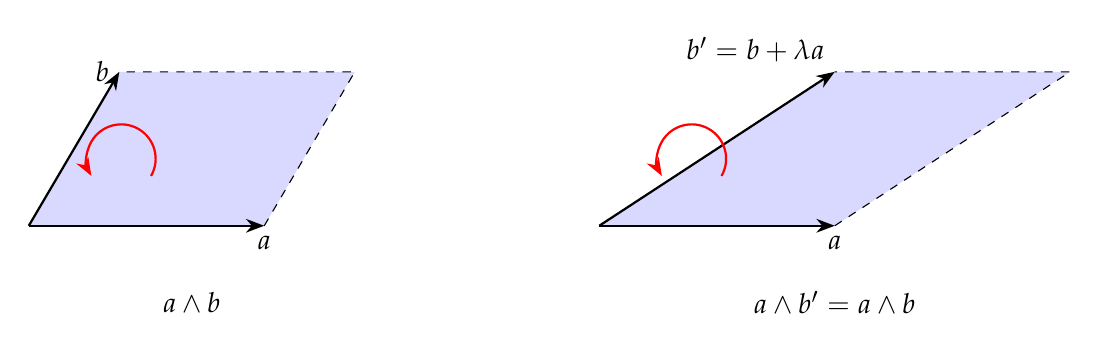
\begin{tikzpicture}[scale=1.15,>=Stealth]
  % left: a wedge b
  \coordinate (O) at (0,0);
  \coordinate (a) at (2.6,0);
  \coordinate (b) at (1.0,1.7);
  \fill[blue!15] (O)--(a)--($(a)+(b)$)--(b)--cycle;
  \draw[thick,->] (O)--(a) node[below]{$a$};
  \draw[thick,->] (O)--(b) node[left]{$b$};
  \draw[dashed] (a)--($(a)+(b)$)--(b);
  \draw[->,red,thick] (1.35,0.55) arc[start angle=-30,end angle=210,radius=0.38];
  \node at (1.8,-0.85) {$a\wedge b$};
  % right: sheared
  \begin{scope}[xshift=6.3cm]
    \coordinate (O) at (0,0);
    \coordinate (a) at (2.6,0);
    \coordinate (b2) at (2.6,1.7); % b + a*(1.6/2.6)... shear
    \fill[blue!15] (O)--(a)--($(a)+(b2)$)--(b2)--cycle;
    \draw[thick,->] (O)--(a) node[below]{$a$};
    \draw[thick,->] (O)--(b2) node[above left]{$b'=b+\lambda a$};
    \draw[dashed] (a)--($(a)+(b2)$)--(b2);
    \draw[->,red,thick] (1.35,0.55) arc[start angle=-30,end angle=210,radius=0.38];
    \node at (2.6,-0.85) {$a\wedge b'=a\wedge b$};
  \end{scope}
\end{tikzpicture}
\caption{The bivector $a\wedge b$ is an oriented area. Shearing $b\mapsto b+\lambda a$ changes the parallelogram but not the bivector, since $a\wedge a=0$.}
\label{fig:wedge}
\end{figure}

\begin{intuition}
\begin{itemize}
  \item A \textbf{vector} is a directed length (an oriented line segment). A \textbf{bivector} $a\wedge b$ is a \emph{directed area}: an
  oriented patch of plane with a magnitude (the area of the parallelogram) and a sense of circulation (go along $a$, then along $b$);
  see Fig.~\ref{fig:wedge}. A \textbf{trivector} $a\wedge b\wedge c$ is an oriented volume, and so on: grade $0,1,2,3,\dots$ = point (scalar), line, plane, volume.
  \item $a\wedge b=0$ exactly when $a,b$ are parallel: the parallelogram is degenerate. This is the algebraic statement that ``zero area'' means ``dependent''.
  \item Only the \emph{plane}, \emph{area} and \emph{orientation} matter, not the particular shape of the parallelogram: $a\wedge(b+\lambda a)=a\wedge b$.
  \item $a\wedge b=-b\wedge a$: reversing the circulation reverses the orientation, just like swapping two columns flips the sign of a determinant (Corollary~\ref{cor:det}: the determinant \emph{is} the volume of the top-grade wedge).
  \item Unlike the cross product, which only exists in $3$D and secretly produces a vector perpendicular to a plane, the wedge works in every dimension and keeps the plane \emph{as a plane}. (We recover the cross product through duality in \S\ref{sec:duality}.)
  \item The exterior algebra knows nothing about lengths or angles: it is metric-free. To also measure, we need the Clifford algebra.
\end{itemize}
\end{intuition}

%% ---- end extract ----


\subsection{The wedge and the tensor product}\label{sec:wedgetensor}

A $k$-tensor on $V$ is a $k$-linear map $V^k\to\R$ with no symmetry condition; these form $T^kV^*=V^*\otimes\cdots\otimes V^*$, of dimension
$n^k$. The tensor product multiplies them by juxtaposition, $(S\otimes T)(v_1,\dots,v_{k+l})=S(v_1,\dots,v_k)\,T(v_{k+1},\dots,v_{k+l})$;
it is associative but not commutative ($\dd x\otimes\dd y\neq\dd y\otimes\dd x$), and it obeys no relations.

\subhead{First description: the wedge is an antisymmetrised tensor product}
Define the antisymmetrisation (alternation) operator
\begin{equation}\label{eq:alt}
(\Alt T)(v_1,\dots,v_k)=\frac1{k!}\sum_{\sigma\in S_k}\sgn(\sigma)\,T\bigl(v_{\sigma(1)},\dots,v_{\sigma(k)}\bigr).
\end{equation}
It is a projection of $T^kV^*$ onto $\bigwedge^kV^*$ ($\Alt T=T$ exactly when $T$ is alternating). Comparing \eqref{eq:alt} for $T=\alpha\otimes\beta$
with \eqref{eq:wedge} gives
\begin{equation}\label{eq:altwedge}
\alpha\wedge\beta=\frac{(k+l)!}{k!\,l!}\,\Alt(\alpha\otimes\beta).
\end{equation}
\numcheck $k=l=1$: $\Alt(\dd x\otimes\dd y)=\tfrac12(\dd x\otimes\dd y-\dd y\otimes\dd x)$ and the prefactor is $2$, so
$\dd x\wedge\dd y=\dd x\otimes\dd y-\dd y\otimes\dd x$.

\begin{pitfall}[a warning on conventions]
Some authors (\eg Kobayashi--Nomizu) drop the factor $(k+l)!/(k!\,l!)$, which gives $\dd x\wedge\dd y=\tfrac12(\dd x\otimes\dd y-\dd y\otimes\dd x)$ and
halves every formula above. The convention of this document for forms (that of Spivak and Lee) is the one for which
$(\dd x^1\wedge\cdots\wedge\dd x^n)(\partial_1,\dots,\partial_n)=1$, so that the volume form really gives volume $1$ to the unit cube.
The embedding of the multivector algebra $\bigwedge V\subset T(V)$ used in Section~\ref{sec:extquotient} uses the other normalisation
($v\wedge w\mapsto\frac12(v\otimes w-w\otimes v)$); the two differ by a factor $k!$ in degree $k$ and are isomorphic as algebras
(Section~\ref{sec:conventions}).
\end{pitfall}

\subhead{Second description: the tensor product with the single rule $\alpha\wedge\alpha=0$}
Let $T(V^*)=\bigoplus_kT^kV^*$ and let $\mathcal I$ be the two-sided ideal generated by all $\alpha\otimes\alpha$ with $\alpha\in V^*$. Then
\begin{equation}\label{eq:extquotient}
\textstyle\bigwedge(V^*)=\bigoplus_k\bigwedge^kV^*\ \cong\ T(V^*)/\mathcal I,\qquad \alpha\wedge\beta=[\alpha\otimes\beta].
\end{equation}
This is the construction of Section~\ref{sec:extquotient} applied to $V^*$. The determinant is the prime example: $\bigwedge^nV^*$ is
one-dimensional, which is why, up to normalisation, there is only one alternating $n$-linear form on $\R^n$.

\subhead{Symmetric versus antisymmetric tensors}
Every $2$-tensor splits uniquely into a symmetric and an antisymmetric part, $V^*\otimes V^*=S^2V^*\oplus\bigwedge^2V^*$,
$T=\tfrac12(T+T^t)+\tfrac12(T-T^t)$. For example
\begin{equation}\label{eq:symantisym}
\dd x\otimes\dd y=\underbrace{\tfrac12(\dd x\otimes\dd y+\dd y\otimes\dd x)}_{\text{symmetric: }\dd x\cdot\dd y}+\underbrace{\tfrac12\,\dd x\wedge\dd y}_{\text{antisymmetric}}.
\end{equation}
\numcheck For $a=(1,2)$, $b=(3,4)$: $(\dd x\otimes\dd y)(a,b)=a^xb^y=4$; the symmetric part is $\frac12(a^xb^y+a^yb^x)=\frac12(4+6)=5$, the antisymmetric part is
$\frac12(4-6)=-1$, and $5+(-1)=4$ \checkmark. Also $(\dd x\wedge\dd y)(a,b)=4-6=-2=2\cdot(-1)$ \checkmark.

The two parts have different jobs. A \emph{metric} is a symmetric $2$-tensor, \eg $g=\dd x\otimes\dd x+\dd y\otimes\dd y$ (written $\dd x^2+\dd y^2$; this ``$\dd x^2$'' is a symmetric
product and has nothing to do with $\dd x\wedge\dd x=0$), and $g(v,v)\neq0$ measures length. A \emph{$2$-form} is an antisymmetric $2$-tensor, and $\omega(v,v)=0$ always; this is why $\iota_v\iota_v=0$ and why the
magnetic force does no work (Section~\ref{sec:phys-em}). For $k\ge3$ the space $T^kV^*$ contains further symmetry types, and $\bigwedge^k$ and $S^k$ are the two extreme ones.

\subhead{Duality with multivectors}
Dually, put $v\wedge w=v\otimes w-w\otimes v\in\bigwedge^2V$ (an oriented parallelogram, or bivector). The pairing of forms with multivectors is again a determinant,
\begin{equation}\label{eq:formmultipairing}
\langle\alpha^1\wedge\cdots\wedge\alpha^k,\ v_1\wedge\cdots\wedge v_k\rangle=\det\bigl[\alpha^i(v_j)\bigr]=(\alpha^1\wedge\cdots\wedge\alpha^k)(v_1,\dots,v_k),
\end{equation}
so contraction \eqref{eq:pairing} extends from $V^*\times V$ to $\bigwedge^kV^*\times\bigwedge^kV$. In this pairing the interior product is the transpose of wedging with $v$:
$\langle\iota_v\alpha,\xi\rangle=\langle\alpha,v\wedge\xi\rangle$ for $\xi\in\bigwedge^{k-1}V$ (this is just definition \eqref{eq:interior} below).

\begin{keyidea}[Why integrands are forms and not arbitrary tensors]
To assign a ``signed volume'' to a parallelepiped $(v_1,\dots,v_k)$ we need: (i) \emph{multilinearity}, so that volumes add when an edge is split;
(ii) \emph{alternation}, so that exchanging two edges flips the orientation and a degenerate (flat) parallelepiped has volume $0$: for a $2$-form $\omega(v,v)=0$ automatically, whereas a general $2$-tensor has $T(v,v)\neq0$ (a metric, for instance);
(iii) the \emph{Jacobian determinant} appearing under changes of variables, which \eqref{eq:detformula} produces by itself. Alternating multilinear maps are exactly $\bigwedge^kV^*\subset T^kV^*$, and the wedge product is the multiplication that keeps one inside this space.
\end{keyidea}

\subsection{The interior product}\label{sec:interior}

For a $k$-form $\alpha$ (an alternating $k$-linear map on tangent vectors) and a vector $v$, the \emph{interior product} (contraction in the first slot) is the $(k-1)$-form
\begin{equation}\label{eq:interior}
(\iota_v\alpha)(w_1,\dots,w_{k-1})=\alpha(v,w_1,\dots,w_{k-1}).
\end{equation}
For $k=1$ this is exactly \eqref{eq:pairing}: $\iota_v\omega=\omega(v)$. The interior product satisfies
\begin{align*}
\iota_v(\alpha\wedge\beta)&=\iota_v\alpha\wedge\beta+(-1)^k\alpha\wedge\iota_v\beta &&\text{(antiderivation, \eqref{eq:antider}),}\\
\iota_v\iota_v&=0, &&\text{($\alpha$ alternating),}\\
\Lie_X&=\dd\,\iota_X+\iota_X\,\dd &&\text{(Cartan's ``magic'' formula, Section~\ref{sec:cartan}).}
\end{align*}

\begin{example}[The interior product in the plane]\label{ex:interiorplane}
The $2$-form $\dd x\wedge\dd y=\dd x\otimes\dd y-\dd y\otimes\dd x$ acts on two vectors $a,b$ as a determinant:
$(\dd x\wedge\dd y)(a,b)=a^xb^y-a^yb^x$. Contract the first slot with $v$ and evaluate on a second vector $w$:
\begin{align*}
\bigl(\iota_v(\dd x\wedge\dd y)\bigr)(w)&=(\dd x\wedge\dd y)(v,w) &&\text{(definition \eqref{eq:interior})}\\
&=v^xw^y-v^yw^x &&\text{(determinant formula)}\\
&=\bigl(v^x\,\dd y-v^y\,\dd x\bigr)(w) &&\text{(since $\dd y(w)=w^y$, $\dd x(w)=w^x$).}
\end{align*}
Hence $\iota_v(\dd x\wedge\dd y)=v^x\,\dd y-v^y\,\dd x$. Two checks: (i) the antiderivation rule gives $\iota_v\dd x\wedge\dd y-\dd x\wedge\iota_v\dd y=v^x\dd y-v^y\dd x$ (same result, using $\iota_v\dd x=v^x$, $\iota_v\dd y=v^y$);
(ii) $\iota_v\iota_v(\dd x\wedge\dd y)=\iota_v(v^x\dd y-v^y\dd x)=v^xv^y-v^yv^x=0$.
\end{example}

The interior product is the bridge between the integration of $1$-forms (Section~\ref{sec:int1}), flux integrals (Section~\ref{sec:intk}) and the Gauss theorem (Section~\ref{sec:gauss}); its metric twin for multivectors is the left contraction of Section~\ref{sec:ops}.

\begin{keypoints}[the exterior algebra]
\begin{itemize}
\item The wedge product is the antisymmetrised tensor product, $\alpha\wedge\beta=\frac{(k+l)!}{k!\,l!}\Alt(\alpha\otimes\beta)$; equivalently the tensor product modulo the single rule $\alpha\wedge\alpha=0$; on $1$-forms it is a determinant, $(\alpha^1\wedge\cdots\wedge\alpha^k)(v_1,\dots,v_k)=\det[\alpha^i(v_j)]$.
\item It is bilinear, associative and graded commutative, $\alpha\wedge\beta=(-1)^{kl}\beta\wedge\alpha$; it detects linear independence, converts changes of basis into determinants (Jacobians), and commutes with pull-back.
\item $\dim\bigwedge^kV^*=\binom nk$; $\bigwedge^n$ is one-dimensional (the volume forms).
\item The exterior algebra needs \emph{no metric}; the interior product $\iota_v$ is the metric-free contraction of forms with vectors.
\end{itemize}
\end{keypoints}


% =====================================================================
\section{The geometric (Clifford) algebra}\label{sec:clifford}
% =====================================================================

The exterior algebra forgets the metric; the geometric algebra puts it back \emph{inside the multiplication}. Instead of
$v\otimes v=0$ we impose $v\otimes v=Q(v)$, the squared length. The remarkable consequence is that the single product $ab$ of two
vectors contains both the dot product (its symmetric part) and the wedge product (its antisymmetric part).
% ---- begin extract GA lines 439-540 ----
Let $(V,Q)$ be a quadratic space, i.e.\ a vector space with a quadratic form $Q$ and its polarization $g$ from \eqref{eq:polar}.

\subsection{Definition by relations}

\begin{definition}[Clifford algebra]
Let $\mathcal I_Q\subset T(V)$ be the two-sided ideal generated by $\{v\otimes v-Q(v)\,1: v\in V\}$. The
\emph{Clifford algebra} is $\Cl(V,Q)=T(V)/\mathcal I_Q$. Its product is called the
\emph{geometric product} and is written by juxtaposition: $uv$. Thus
\begin{equation}\label{eq:cliff}
 v\,v=Q(v)=v\cdot v\qquad\text{for every }v\in V.
\end{equation}
When $V=\R^{p,q}$ we write $\Cl(p,q)$; the algebra is then also called the \emph{geometric algebra} $\GA(V)$ and its elements \emph{multivectors}.
\end{definition}

\begin{theorem}[Universal property]\label{thm:cliffuniv}
Let $A$ be a unital associative algebra and $f:V\to A$ linear with $f(v)^2=Q(v)1_A$ for all $v$. Then $f$ extends uniquely to an algebra homomorphism $\Cl(V,Q)\to A$.
\end{theorem}
\begin{proof}
By Theorem~\ref{thm:Tuniv}, $f$ extends to $\bar f:T(V)\to A$; the hypothesis says $\bar f$ kills each generator $v\otimes v-Q(v)$ of $\mathcal I_Q$, hence all of $\mathcal I_Q$, so $\bar f$ descends to the quotient.
\end{proof}

\begin{proposition}[Fundamental identity]\label{prop:fund}
For $u,v\in V$: $\;uv+vu=2\,g(u,v)=2\,u\cdot v$. In particular, orthogonal vectors anticommute.
\end{proposition}
\begin{proof}
Polarize \eqref{eq:cliff}: $(u+v)^2-u^2-v^2=uv+vu$, and by \eqref{eq:polar} this equals $2g(u,v)$.
\end{proof}

Hence, for an orthonormal basis $(e_i)$ with $e_i^2=\varepsilon_i=\pm1$, the \emph{entire} algebra is generated by the relations
\[
 e_ie_j=-e_je_i\ (i\neq j),\qquad e_i^2=\varepsilon_i .
\]

\subsection{Size of the algebra and relation to $\bigwedge V$}

\begin{theorem}[Dimension, basis]\label{thm:cliffbasis}
$\dim\Cl(V,Q)=2^n$, with basis $e_I=e_{i_1}e_{i_2}\cdots e_{i_k}$ for $I=\{i_1<\cdots<i_k\}\subseteq\{1,\dots,n\}$ (and $e_\emptyset=1$).
\end{theorem}
\begin{proof}[Proof sketch]
\emph{Upper bound.} Using $e_ie_j=-e_je_i$ and $e_i^2=\varepsilon_i$, any word can be reordered into $\pm$ (a scalar) $\cdot\,e_I$ for some $I$, so the $e_I$ span.
\emph{Lower bound (Chevalley's construction).} For $v\in V$ let $\iota_v$ be the \emph{interior product} on $\bigwedge V$: the unique antiderivation of degree $-1$ with $\iota_v(w)=g(v,w)$ for $w\in V$. Define
$\rho(v)\,\omega=v\wedge\omega+\iota_v\omega$ on $\bigwedge V$. Using $\iota_v(v\wedge\omega)=g(v,v)\omega-v\wedge\iota_v\omega$ and $\iota_v^2=0$, $v\wedge v=0$ one finds
\[
 \rho(v)^2\omega=v\wedge\iota_v\omega+\iota_v(v\wedge\omega)=Q(v)\,\omega .
\]
By Theorem~\ref{thm:cliffuniv}, $\rho$ extends to an algebra map $\Cl(V,Q)\to\mathrm{End}(\bigwedge V)$. The map $x\mapsto\rho(x)1$ sends $e_I\mapsto e_{i_1}\wedge\cdots\wedge e_{i_k}$ (for an orthogonal basis the interior terms vanish), which are linearly independent by Theorem~\ref{thm:extbasis}. Hence the $e_I$ are independent.
\end{proof}

\begin{corollary}[Grades]\label{cor:grades}
The map $\bigwedge V\to\Cl(V,Q)$ given by antisymmetrization,
\[
 v_1\wedge\cdots\wedge v_k\;\longmapsto\;\frac1{k!}\sum_{\sigma\in S_k}\sgn(\sigma)\,v_{\sigma(1)}v_{\sigma(2)}\cdots v_{\sigma(k)},
\]
is a (basis-independent) linear isomorphism of vector spaces. We use it to write $\GA(V)=\bigoplus_{k=0}^n\GA^k(V)$ and to define the
\emph{grade projections} $\gr{A}{k}$. For \emph{mutually orthogonal} vectors, $a_1a_2\cdots a_k=a_1\wedge\cdots\wedge a_k$. The product does \emph{not} preserve grade, but it preserves the parity (even/odd), so the \emph{even part} $\GA^+=\bigoplus_{k\ \mathrm{even}}\GA^k$ is a subalgebra.
\end{corollary}

\begin{remark}
So, as vector spaces, $\Cl(V,Q)\cong\bigwedge V$; they differ only in the \emph{multiplication}. When $Q=0$ the Clifford algebra is the exterior algebra. In this sense the Clifford algebra is a \emph{deformation} of $\bigwedge V$ by the metric.
\end{remark}

\subsection{Examples}

\begin{example}[Low-dimensional algebras] Write $\Cl(p,q)$ for $p$ basis vectors squaring to $+1$ and $q$ to $-1$.
\begin{itemize}
  \item $\Cl(0,1)$: one generator $e$ with $e^2=-1$; basis $\{1,e\}$; $\Cl(0,1)\cong\C$.
  \item $\Cl(1,0)\cong\R\oplus\R$ (the split-complex numbers, $e^2=+1$).
  \item $\Cl(2,0)$: basis $\{1,e_1,e_2,e_1e_2\}$; $(e_1e_2)^2=-e_1^2e_2^2=-1$; $\Cl(2,0)\cong\Mat_2(\R)$.
  \item $\Cl(0,2)$: with $i=e_1$, $j=e_2$, $k=e_1e_2$ one gets the quaternions: $\Cl(0,2)\cong\Hq$.
  \item $\Cl(3,0)$: dimension $8$; the Pauli matrices $e_i\mapsto\sigma_i$ give $\Cl(3,0)\cong\Mat_2(\C)$.
  \item $\Cl(1,3)$ (spacetime algebra, $e_0^2=+1$, $e_i^2=-1$) has dimension $16$ and is $\cong\Mat_2(\Hq)$.
\end{itemize}
\end{example}

\subsection{The geometric product of two vectors}

\begin{proposition}\label{prop:abdecomp}
For $a,b\in V$,
\begin{equation}\label{eq:abdecomp}
 ab=a\cdot b+a\wedge b,\qquad a\cdot b=\tfrac12(ab+ba),\quad a\wedge b=\tfrac12(ab-ba).
\end{equation}
The wedge here coincides with the exterior product under the identification of Corollary~\ref{cor:grades}.
\end{proposition}
\begin{proof}
Write $ab=\tfrac12(ab+ba)+\tfrac12(ab-ba)$. The first term is $a\cdot b$ by Proposition~\ref{prop:fund}; the second is the antisymmetrization of Corollary~\ref{cor:grades} for $k=2$.
\end{proof}

Every nonzero vector $a$ with $a^2\neq0$ is \emph{invertible}: $a^{-1}=a/a^2$. Consequently equations such as $ax=b$ can be solved by \emph{division}: $x=a^{-1}b$. (Neither the dot product nor the cross product allows this.)

\begin{intuition}
Decompose $b=b_\parallel+b_\perp$ with $b_\parallel=(a\cdot b)\,a^{-1}$ the part along $a$ and $b_\perp$ the part orthogonal to $a$.
Then $ab_\parallel=a\cdot b$ is a scalar (a vector times a parallel vector is a pure number: it is the \emph{projection} information) while
$ab_\perp=a\wedge b$ is a pure bivector (a vector times a perpendicular vector is an oriented area: it is the \emph{rejection} information).
So the geometric product $ab$ is a single object that remembers \emph{how parallel} and \emph{how perpendicular} two vectors are.
In the Euclidean case
\[
 ab=|a||b|\bigl(\cos\theta+\hat B\sin\theta\bigr),\qquad \hat B=\frac{a\wedge b}{|a\wedge b|},\quad \hat B^2=-1,
\]
which is the exact analogue of $e^{i\theta}=\cos\theta+i\sin\theta$ with the imaginary unit replaced by the \emph{plane} spanned by $a,b$.
In the plane, $i\equiv e_1e_2$ and $i^2=-1$ appear \emph{naturally}, not as an ad-hoc construction, and in any dimension every oriented plane carries its own ``imaginary unit''.
\end{intuition}

%% ---- end extract ----


% =====================================================================
\section{Operations on multivectors}\label{sec:ops}
% =====================================================================

The geometric product induces a family of derived operations: grade projections, three involutions, and the inner, outer and
contraction products. The left contraction $a\lc A$ is the metric incarnation of the interior product $\iota_a$ of
Section~\ref{sec:interior} (Section~\ref{sec:synth1} makes the identification precise).
% ---- begin extract GA lines 544-606 ----

\subsection{Involutions}

\begin{definition}
On $\GA(V)$ define:
\begin{itemize}
  \item the \emph{grade involution} $\hat A$: the algebra automorphism with $\hat v=-v$. On a $k$-vector, $\hat A=(-1)^kA$.
  \item the \emph{reverse} $\rev A$: the algebra \emph{anti}-automorphism ($\rev{AB}=\rev B\,\rev A$) with $\rev v=v$. On a $k$-vector, $\rev A=(-1)^{k(k-1)/2}A$ (reversing the order of the factors in $a_1\cdots a_k$).
  \item the \emph{Clifford conjugate} $\bar A=\rev{\hat A}$.
\end{itemize}
\end{definition}

The reverse has signs $+,+,-,-,+,+,\dots$ for grades $0,1,2,3,4,5,\dots$ In particular bivectors satisfy $\rev B=-B$.

\subsection{Inner, outer and contraction products}

\begin{definition}[Products induced by the geometric product]\label{def:products}
For homogeneous multivectors $A_r\in\GA^r$ and $B_s\in\GA^s$:
\begin{align*}
 A_r\wedge B_s&:=\gr{A_rB_s}{r+s}&&\text{(outer product)},\\
 A_r\lc B_s&:=\gr{A_rB_s}{s-r}&&\text{(left contraction; $=0$ if $r>s$)},\\
 A_r*B_s&:=\gr{A_rB_s}{0}&&\text{(scalar product)},
\end{align*}
extended bilinearly to all multivectors. The squared norm (Euclidean case) is $\norm A^2=\gr{A\rev A}{0}\ge0$.
\end{definition}

For a vector $a$ and an $r$-vector $A_r$ one has the explicit formulas
\begin{equation}\label{eq:aA}
 aA_r=a\lc A_r+a\wedge A_r,\qquad
 a\lc A_r=\tfrac12\bigl(aA_r-(-1)^rA_ra\bigr),\quad
 a\wedge A_r=\tfrac12\bigl(aA_r+(-1)^rA_ra\bigr),
\end{equation}
of grades $r-1$ and $r+1$ respectively (for $r=1$ this is \eqref{eq:abdecomp}).

\begin{proposition}[Properties]\label{prop:contr}
For $a\in V$ and multivectors $A,B,C$:
\begin{enumerate}
  \item (explicit formula) $a\lc(b_1\wedge\cdots\wedge b_k)=\sum_{i=1}^k(-1)^{i-1}(a\cdot b_i)\,b_1\wedge\cdots\wedge\widehat{b_i}\wedge\cdots\wedge b_k$.
  \item (antiderivation) $a\lc(A_s\wedge B)=(a\lc A_s)\wedge B+(-1)^sA_s\wedge(a\lc B)$.
  \item (associativity-type identity) $A\lc(B\lc C)=(A\wedge B)\lc C$.
  \item $(A\wedge B)\wedge C=A\wedge(B\wedge C)$, and $A_r\wedge B_s=(-1)^{rs}B_s\wedge A_r$.
\end{enumerate}
\end{proposition}
\begin{proof}[Proof idea]
(1) and (2) follow by induction from \eqref{eq:aA} (for $k=2$: $a\lc(b\wedge c)=(a\cdot b)c-(a\cdot c)b$). (3) is checked first for $A=a$ a vector, using (2), and then holds by induction on the grade of $A$. (4) is the statement that the wedge defined here agrees with the exterior product of \S\ref{sec:ext} (Corollary~\ref{cor:grades}).
\end{proof}

\begin{example}
$a\lc(b\wedge c)=(a\cdot b)\,c-(a\cdot c)\,b$ is a vector lying in the plane $b\wedge c$ and perpendicular to $a$: indeed $a\cdot\bigl((a\cdot b)c-(a\cdot c)b\bigr)=0$.
\end{example}

\begin{remark}[Commutator product]
For bivectors $A,B$ one has $AB=A\lc B+\tfrac12(AB-BA)+A\wedge B$ with the three terms of grades $0,2,4$. The antisymmetric middle part, $A\times B:=\tfrac12(AB-BA)$ is again a bivector; it makes $\GA^2$ a Lie algebra isomorphic to $\mathfrak{so}(p,q)$.
\end{remark}

\begin{intuition}
\begin{itemize}
  \item \textbf{Wedge = ``span''.} $A\wedge B$ builds the higher-dimensional element containing both (it is $0$ if they share a direction). It is the \emph{join}.
  \item \textbf{Contraction = ``the part of $B$ perpendicular to $A$, measured by $A$''.} $a\lc B$ removes the direction $a$ from the blade $B$ and returns what remains inside $B$, perpendicular to $a$, with the scale of $|a|$. It lowers grade by one.
  \item \textbf{Geometric product = both at once.} For a vector $a$ and blade $B$, $aB=a\lc B+a\wedge B$ splits into the \emph{lower}-grade part (the part of $a$ lying inside $B$) and the \emph{higher}-grade part (the part of $a$ sticking out of $B$). Because the splitting is a sum of different grades, no information is lost, and that is why $a$ can be divided out again.
\end{itemize}
\end{intuition}

%% ---- end extract ----


% =====================================================================
\section{Reflections, rotations and rotors}\label{sec:rotors}
% =====================================================================
% ---- begin extract GA lines 610-667 ----

\begin{theorem}[Reflections]\label{thm:refl}
Let $n\in V$ be invertible ($n^2\neq0$). The map $x\mapsto -nxn^{-1}$ is the reflection of $V$ across the hyperplane orthogonal to $n$.
\end{theorem}
\begin{proof}
Decompose $x=x_\parallel+x_\perp$, $x_\parallel=(x\cdot n)n^{-1}$ parallel to $n$, $x_\perp\cdot n=0$. Then $nx_\parallel=x_\parallel n$ (parallel vectors commute) and $nx_\perp=-x_\perp n$ (Proposition~\ref{prop:fund}). Hence
$-nxn^{-1}=-x_\parallel+x_\perp$.
\end{proof}

\begin{definition}[Versors, Pin and Spin]
A \emph{versor} is a product $U=v_1v_2\cdots v_k$ of invertible vectors. It acts on $V$ by
$x\mapsto(-1)^k\,UxU^{-1}$, which is an orthogonal transformation (a composition of $k$ reflections). The versors with $U\rev U=\pm1$ form the group $\Pin(V,Q)$ and the even ones form $\Spin(V,Q)=\Pin\cap\GA^+$. An even versor $R$ with $R\rev R=1$ is called a \emph{rotor}; it acts by the \emph{sandwich product}
\[
 x\longmapsto RxR^{-1}=Rx\rev R .
\]
\end{definition}

By the Cartan--Dieudonn\'e theorem every orthogonal transformation of an $n$-dimensional space is a product of at most $n$ reflections. Hence every rotation arises from a rotor, and $R$ and $-R$ give the same rotation (the \emph{double cover} $\Spin\to SO$).

\begin{theorem}[Rotors in a plane]\label{thm:rotor}
Let $B$ be a unit bivector with $B^2=-1$ (a blade representing an oriented plane in Euclidean space). Then
\[
 R=e^{-\varphi B/2}=\cos\tfrac\varphi2-B\sin\tfrac\varphi2
\]
acts by $x\mapsto Rx\rev R$ as the rotation by angle $\varphi$ in the plane of $B$, in the orientation of $B$, leaving the orthogonal complement of the plane fixed.
\end{theorem}
\begin{proof}
Split $x=x_\parallel+x_\perp$ into the part in the plane of $B$ and the part orthogonal to it. A vector in the plane anticommutes with $B$ (e.g.\ $e_1e_1e_2=-e_1e_2e_1$), hence $e^{-\varphi B/2}x_\parallel=x_\parallel e^{\varphi B/2}$ and
$Rx_\parallel\rev R=x_\parallel e^{\varphi B/2}e^{\varphi B/2}=x_\parallel e^{\varphi B}$. For $B=e_1e_2$ and $x_\parallel=e_1$ this gives $e_1(\cos\varphi+e_1e_2\sin\varphi)=\cos\varphi\,e_1+\sin\varphi\,e_2$. A vector orthogonal to the plane commutes with $B$, so $Rx_\perp\rev R=x_\perp R\rev R=x_\perp$.
\end{proof}

\begin{figure}[ht]
\centering
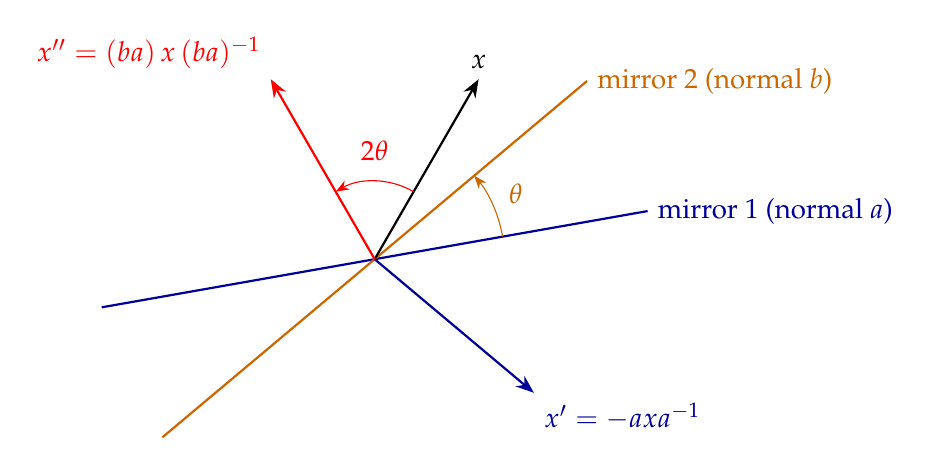
\begin{tikzpicture}[>=Stealth,scale=1.1]
  \draw[thick,blue!60!black] (190:3.2)--(10:3.2) node[right]{mirror $1$ (normal $a$)};
  \draw[thick,orange!80!black] (220:3.2)--(40:3.2) node[right]{mirror $2$ (normal $b$)};
  \draw[->,thick] (0,0)--(60:2.4) node[above]{$x$};
  \draw[->,thick,blue!60!black] (0,0)--(-40:2.4) node[below right]{$x'=-axa^{-1}$};
  \draw[->,thick,red] (0,0)--(120:2.4) node[above left]{$x''=(ba)\,x\,(ba)^{-1}$};
  \draw[red,->] (60:0.9) arc[start angle=60,end angle=120,radius=0.9];
  \node[red] at (90:1.25) {$2\theta$};
  \draw[orange!80!black,->] (10:1.5) arc[start angle=10,end angle=40,radius=1.5];
  \node[orange!80!black] at (25:1.8) {$\theta$};
\end{tikzpicture}
\caption{Two reflections compose to a rotation by \emph{twice} the angle $\theta$ between the mirrors. The rotor is $R=ba=e^{-B\theta}$.}
\label{fig:tworefl}
\end{figure}

\begin{intuition}
A reflection is the simplest orthogonal map, and a rotation is just \emph{two reflections in a row} (Fig.~\ref{fig:tworefl}); this is a classical fact of plane geometry.
Algebraically, reflecting first in $a$ and then in $b$ gives $x\mapsto b(-axa^{-1})b^{-1}=(ba)x(ba)^{-1}$, so the \emph{product of the two mirror vectors} $R=ba$ \emph{is} the rotation.
Since the rotation angle is twice the angle between the mirrors, the rotor contains the \emph{half-angle} $\varphi/2$; that is where the half angles of quaternions and spinors come from. The rotor is also dimension-free: no ``axis of rotation'' is needed (axes exist only in $3$D), only the \emph{plane} of rotation, which is the bivector $B$. Composing rotations is just multiplying rotors: $R_2R_1$.
\end{intuition}

\begin{example}[Quaternions inside $\Cl(3,0)$]
In $\GA(\R^3)$ put $i=e_3e_2$, $j=e_1e_3$, $k=e_2e_1$. Then $i^2=j^2=k^2=-1$ and $ij=k$ (direct computation), so the even subalgebra $\GA^+(\R^3)=\{\alpha+\text{bivector}\}$ is the quaternion algebra $\Hq$. Unit quaternions are exactly the rotors of $\R^3$, and $x\mapsto qxq^{-1}$ is the usual quaternion rotation. The pseudoscalar $e_1e_2e_3$ will play the role of the ``axis'' in \S\ref{sec:duality}.
\end{example}

%% ---- end extract ----


% =====================================================================
\section{Duality: the pseudoscalar, the dual, the cross product and the Hodge star}\label{sec:duality}
% =====================================================================

The pseudoscalar $\pss$ (the unit $n$-vector) gives each multivector a perpendicular partner of complementary grade. This
single idea explains the cross product, the Hodge star, ``axial'' vectors and the grad--curl--div pattern met later.
% ---- begin extract GA lines 671-789 ----

\subsection{The pseudoscalar}

Let $(e_1,\dots,e_n)$ be an orthonormal basis of a non-degenerate space $V=\R^{p,q}$.

\begin{definition}[Pseudoscalar]
The \emph{unit pseudoscalar} is $\pss=e_1e_2\cdots e_n=e_1\wedge\cdots\wedge e_n\in\GA^n(V)$. Changing the basis by an orientation-preserving orthogonal map leaves $\pss$ unchanged; an orientation-reversing one changes its sign. Choosing $\pss$ is therefore the same as choosing an \emph{orientation} of $V$.
\end{definition}

\begin{proposition}\label{prop:pss}
\begin{enumerate}
  \item $\pss^2=(-1)^{n(n-1)/2}(-1)^q$ and $\pss^{-1}=\rev\pss/(\pss\rev\pss)$. In the Euclidean case $\pss^{-1}=\rev\pss=(-1)^{n(n-1)/2}\pss$.
  \item $e_i\pss=(-1)^{n-1}\pss e_i$: $\pss$ commutes with all vectors if $n$ is odd, and anticommutes with them if $n$ is even. In particular $\pss$ is central in $\GA(V)$ when $n$ is odd.
  \item For any $k$-vector $A$ the product $A\pss$ is a pure $(n-k)$-vector.
\end{enumerate}
\end{proposition}
\begin{proof}
(1) $\rev\pss=e_n\cdots e_1=(-1)^{n(n-1)/2}\pss$ and $\pss\rev\pss=\prod_i e_i^2=(-1)^q$, so $\pss^2=(-1)^{n(n-1)/2}\pss\rev\pss$. (2) Moving $e_i$ through $\pss$ it anticommutes with the $n-1$ factors $e_j$, $j\neq i$, and commutes with $e_i$. (3) For a basis blade $e_J$ with $|J|=k$, $e_J\pss$ equals, up to a sign and a product of $\varepsilon_j$, the basis blade $e_{J^c}$ of the complementary indices.
\end{proof}

\subsection{The dual}

\begin{definition}[Dual and undual]\label{def:dual}
The \emph{dual} of a multivector $A$ is
\[
 \dual A:=A\,\pss^{-1}\;=\;A\lc\pss^{-1},
\]
and the \emph{undual} is $A\mapsto A\pss$. (The two operations differ from each other only by the scalar factor $\pss^{2}$: $A\pss=\pss^2\,\dual A$.)
\end{definition}

\begin{theorem}[Properties of the dual]\label{thm:dual}
\begin{enumerate}
  \item $A\mapsto\dual A$ is a linear isomorphism $\GA^k(V)\to\GA^{n-k}(V)$, and $\dual{(\dual A)}=\pss^{-2}A=\pm A$.
  \item (\emph{Orthogonal complement}) If $A$ is a $k$-blade representing the subspace $U\subset V$, then $\dual A$ is an $(n-k)$-blade representing the orthogonal complement $U^\perp$ and $\norm{\dual A}=\norm A$ (Euclidean case).
  \item (\emph{Wedge $\leftrightarrow$ contraction}) For all multivectors $A,B$,
  \begin{equation}\label{eq:dualduality}
   \dual{(A\wedge B)}=A\lc\dual B,\qquad \dual{(A\lc B)}=A\wedge\dual B .
  \end{equation}
\end{enumerate}
\end{theorem}
\begin{proof}
(1) follows from Proposition~\ref{prop:pss}(3) and invertibility of $\pss$.
(2) Choose an orthonormal basis adapted to $U$ so that (after scaling) $A=e_1\cdots e_k$. Then $\pss^{-1}=e_n^{-1}\cdots e_{k+1}^{-1}\,e_k^{-1}\cdots e_1^{-1}$ and, since the $(n-k)$-blade $e_n^{-1}\cdots e_{k+1}^{-1}$ is built from vectors orthogonal to $e_1,\dots,e_k$, it commutes with $A$ up to $(-1)^{k(n-k)}$. Hence $A\pss^{-1}=(-1)^{k(n-k)}e_n^{-1}\cdots e_{k+1}^{-1}$, a blade spanning $U^\perp$.
(3) For homogeneous $B$ we have $B\lc\pss^{-1}=B\pss^{-1}$ (the product has the single grade $n-\deg B$). Proposition~\ref{prop:contr}(3) gives
$A\lc(B\pss^{-1})=A\lc(B\lc\pss^{-1})=(A\wedge B)\lc\pss^{-1}=\dual{(A\wedge B)}$, the first identity. For the second, apply the first to $A$ and $B'=B\pss$ (so $\dual{B'}=B$): $A\lc B=\dual{(A\wedge B\pss)}$; then $\dual{(A\lc B)}=(A\wedge B\pss)\pss^{-2}=A\wedge(B\pss^{-1})=A\wedge\dual B$, using that $\pss^{2}$ is a scalar.
\end{proof}

\begin{corollary}[Meet and the regressive product]\label{cor:meet}
Define the \emph{meet} (regressive product)
\[
 A\meet B:=(\dual B\wedge\dual A)\,\pss=\dual B\lc A .
\]
If $A,B$ are blades whose subspaces $U_A,U_B$ have $U_A+U_B=V$, then $A\meet B$ is (a multiple of) the blade of $U_A\cap U_B$.
\end{corollary}
\begin{proof}
$U_A^\perp$ and $U_B^\perp$ span $(U_A\cap U_B)^\perp$ when $U_A+U_B=V$, so $\dual B\wedge\dual A$ represents $(U_A\cap U_B)^\perp$ by Theorem~\ref{thm:dual}(2), and undualizing gives $U_A\cap U_B$. The equality of the two expressions follows from \eqref{eq:dualduality}: $(\dual B\wedge\dual A)\pss=\pss^2\,\dual{(\dual B\wedge\dual A)}=\pss^2\,\dual B\lc\dual{(\dual A)}=\dual B\lc A$.
\end{proof}

\begin{example}[Meet of two planes in $\R^3$]
$A=e_1e_2$ and $B=e_2e_3$ (the $xy$- and $yz$-planes). With $\pss=e_1e_2e_3$, $\pss^{-1}=-\pss$ one finds $\dual A=e_3$, $\dual B=e_1$, and $A\meet B=\dual B\lc A=e_1\lc(e_1e_2)=e_2$: the $y$-axis, the line of intersection.
\end{example}

\subsection{The cross product, rotation axes, and complex numbers}

\begin{proposition}[Cross product]\label{prop:cross}
In $\GA(\R^3)$ with $\pss=e_1e_2e_3$ (so $\pss^2=-1$, $\pss$ central),
\[
 a\times b=\dual{(a\wedge b)}=(a\wedge b)\pss^{-1}=-\pss\,(a\wedge b),\qquad\text{equivalently}\qquad a\wedge b=\pss\,(a\times b).
\]
\end{proposition}
\begin{proof}
By bilinearity check on the basis: $e_1e_2\pss^{-1}=-e_1e_2e_1e_2e_3=e_3=e_1\times e_2$, and cyclically for $e_2e_3,e_3e_1$.
\end{proof}

Hence \emph{the cross product is the dual of the wedge}. It exists only in $n=3$ because that is when the dual of a bivector ($n-2$) is a vector ($1$). It is also why $a\times b$ is a ``pseudovector'': it changes sign under an orientation reversal, because the dual depends on $\pss$.

\begin{example}[Rotation about an axis]
The plane perpendicular to a unit vector $m\in\R^3$, oriented by the right-hand rule, is $B=\pss m$ (e.g.\ $\pss e_3=e_1e_2$). Theorem~\ref{thm:rotor} gives the rotation by $\varphi$ about the axis $m$:
\[
 R=\exp\!\bigl(-\tfrac\varphi2\,\pss m\bigr)=\cos\tfrac\varphi2-\pss m\,\sin\tfrac\varphi2,\qquad x\mapsto Rx\rev R .
\]
In $2$D, $\pss=e_1e_2$ acts as the imaginary unit and the dual of a vector is that vector turned by a quarter turn.
\end{example}

\subsection{Relation to the Hodge star and to the dual space}

Let $V$ be Euclidean and oriented, with the inner product on $\bigwedge^kV$ for which $\{e_I\}$ is orthonormal; in terms of the geometric product, $\langle A,B\rangle=\gr{\rev AB}{0}$.

\begin{definition}[Hodge star]
The \emph{Hodge star} $\hodge:\bigwedge^kV\to\bigwedge^{n-k}V$ is defined by
\[
 \alpha\wedge\hodge\beta=\langle\alpha,\beta\rangle\,\pss\qquad\text{for all }\alpha,\beta\in\textstyle\bigwedge^kV .
\]
\end{definition}

\begin{theorem}\label{thm:hodgeGA}
For a $k$-vector $A$ in the Euclidean case,
\[
 \hodge A=\rev A\,\pss=(-1)^{k(k-1)/2+n(n-1)/2}\,\dual A .
\]
So the Hodge star and the geometric-algebra dual agree up to a grade-dependent sign. Moreover $\hodge\hodge=(-1)^{k(n-k)}$ on $k$-vectors.
\end{theorem}
\begin{proof}
For an orthonormal basis blade $e_J$ ($|J|=k$) we have $\rev{e_J}=e_J^{-1}$. Then $e_J\wedge(\rev{e_J}\pss)=e_J\,e_J^{-1}\pss=\pss$, since the product of $e_J$ with the complementary blade $e_J^{-1}\pss$ (built from the other basis vectors) is a wedge; and $e_{J'}\wedge(\rev{e_J}\pss)=0$ for $J'\neq J$ because the indices overlap. This is precisely the defining property of $\hodge e_J$. The sign relation follows from $\rev A=(-1)^{k(k-1)/2}A$ and $\pss^{-1}=(-1)^{n(n-1)/2}\pss$.
\end{proof}

\begin{remark}[The ``other'' dual]
The word \emph{dual} has two meanings that are connected here. The \emph{dual space} $V^*$ is intrinsically defined, whereas $V\cong V^*$ needs the metric ($\flat$). Intrinsically, the wedge pairing $\bigwedge^kV\times\bigwedge^{n-k}V\to\bigwedge^nV\cong\K$ is perfect, so $\bigwedge^{n-k}V\cong(\bigwedge^kV)^*$ once a basis (orientation and volume) $\pss$ of $\bigwedge^nV$ is chosen. Combined with the metric identification $(\bigwedge^kV)^*\cong\bigwedge^kV$, this is exactly the map $A\mapsto\dual A$ (or $\hodge A$). The pseudoscalar $\pss$ packages \emph{both} the orientation and the metric volume.
\end{remark}

\begin{intuition}
\begin{itemize}
  \item \textbf{Dual = orthogonal complement.} Every subspace has a perpendicular partner: a plane in $3$D has a normal line, a line has a normal plane. The dual swaps a $k$-dimensional oriented subspace with its $(n-k)$-dimensional partner (and keeps the magnitude).
  Describing a plane \emph{by its normal} or \emph{by its tangent bivector} are two views of the same object; the dual converts between them (for example $e_1\wedge e_2\leftrightarrow e_3$ in $\R^3$).
  \item \textbf{Wedge $\leftrightarrow$ meet.} The wedge joins subspaces (spans). In the dual picture it becomes a contraction/meet (intersections). The identity $\dual{(A\wedge B)}=A\lc\dual B$ says that ``the complement of a span is what is left perpendicular to both''. Intersections of planes, lines and so on, without coordinates.
  \item \textbf{The pseudoscalar is the orientation of space.} Multiplying by $\pss^{-1}$ is a ``quarter-turn of the whole space'': in 2D it is multiplication by $\pm i$; in 3D it turns planes into axes. Reversing the orientation flips the sign of the dual; this is why the cross product is a \emph{pseudo}vector and the magnetic field $B$ is better treated as a \emph{bivector}.
\end{itemize}
\end{intuition}

%% ---- end extract ----


% =====================================================================
\section{Synthesis I: contraction, duality and the role of the metric}\label{sec:synth1}
% =====================================================================

\begin{synthesis}[what this section does]
Three languages have now appeared for the same linear algebra: \emph{index} (tensor) notation, \emph{forms} on $V^*$, and \emph{multivectors} in $V$. This
section lines them up. It answers three questions: which of the ``contractions'' are really the same operation
(Section~\ref{sec:contr4}), which operations genuinely need a metric (Section~\ref{sec:whichmetric}), and how the
conventions of the different sources are reconciled (Section~\ref{sec:conventions}).
\end{synthesis}

\subsection{Contraction in four guises}\label{sec:contr4}

The word ``contraction'' has been used four times; they are one idea at four levels of structure.

\begin{center}
\small
\renewcommand{\arraystretch}{1.35}
\begin{tabular}{@{}p{3.4cm}p{3.5cm}p{4.2cm}p{2.2cm}@{}}
\toprule
\textbf{Guise} & \textbf{Acts on} & \textbf{Formula} & \textbf{Metric?}\\
\midrule
Evaluation $\langle\omega,v\rangle$ & $V^*\times V\to\R$ & $\omega_iv^i$ & no\\
Tensor contraction & $T^{\ell}_{k}\to T^{\ell-1}_{k-1}$ & trace $A^i{}_i$; $f_iv^i$; Ricci $R^i{}_{ijk}$ & no\\
Interior product $\iota_v$ & $k$-forms $\to(k-1)$-forms & $(\iota_v\alpha)(w_\bullet)=\alpha(v,w_\bullet)$ & no\\
Left contraction $a\lc A$ & $k$-vectors $\to(k-1)$-vectors & $a\lc(b\wedge c)=(a\!\cdot\! b)c-(a\!\cdot\! c)b$ & yes ($\cdot$ is $g$)\\
\bottomrule
\end{tabular}
\end{center}

The first three need only $V$ and $V^*$. The fourth acts on vectors and needs a metric, but it is the \emph{same} operation as the third once a
metric is available to translate between $V$ and $V^*$:

\begin{proposition}[left contraction $=$ interior product under $\flat$]\label{prop:lcisiota}
Extend $\flat:V\to V^*$ to an algebra homomorphism of exterior algebras, $(v_1\wedge\cdots\wedge v_k)^\flat=v_1^\flat\wedge\cdots\wedge v_k^\flat$. Then for every $a\in V$
and every multivector $A$,
\[
(a\lc A)^\flat=\iota_a\bigl(A^\flat\bigr).
\]
\end{proposition}
\begin{proof}
Both sides are antiderivations in $A$ of degree $-1$ (for $a\lc$, see the properties in Section~\ref{sec:ops}; for $\iota_a$, \eqref{eq:antider}). On a vector $b$ they agree:
$(a\lc b)^\flat=(a\cdot b)=g(a,b)=b^\flat(a)=\iota_a b^\flat$. Since multivectors are sums of wedges of vectors, an induction on the grade using the antiderivation rule shows that they agree everywhere.
\end{proof}

\begin{example}[the three-vector check]\label{ex:lcvsiota}
Take $a,b,c\in\R^3$ with the Euclidean metric. Then $(a\lc(b\wedge c))^\flat=\bigl((a\!\cdot\!b)c-(a\!\cdot\!c)b\bigr)^\flat=(a\!\cdot\!b)c^\flat-(a\!\cdot\!c)b^\flat$, and
$\iota_a(b^\flat\wedge c^\flat)=b^\flat(a)\,c^\flat-c^\flat(a)\,b^\flat$ by \eqref{eq:wedge11}; the two agree because $b^\flat(a)=a\cdot b$. In coordinates this is exactly
the planar computation of Example~\ref{ex:interiorplane}: $\iota_v(\dd x\wedge\dd y)=v^x\dd y-v^y\dd x$.
\end{example}

\begin{synthesis}[the same identities, three notations]
\renewcommand{\arraystretch}{1.3}
\begin{center}\small
\begin{tabular}{@{}p{3.6cm}p{4.0cm}p{4.0cm}@{}}
\toprule
\textbf{Fact} & \textbf{Forms} & \textbf{Multivectors}\\
\midrule
antiderivation & $\iota_v(\alpha\wedge\beta)=\iota_v\alpha\wedge\beta+(-1)^k\alpha\wedge\iota_v\beta$ & $a\lc(A_k\wedge B)=(a\lc A_k)\wedge B+(-1)^kA_k\wedge(a\lc B)$\\
nilpotent & $\iota_v\iota_v=0$ & $a\lc(a\lc A)=(a\wedge a)\lc A=0$\\
wedge is not metric & $\alpha\wedge\beta$ & $A\wedge B$ (grade part of $AB$, but defined without $g$)\\
\bottomrule
\end{tabular}
\end{center}
\end{synthesis}

\subsection{Which operations need a metric?}\label{sec:whichmetric}

The divisions drawn in Sections~\ref{sec:metric}--\ref{sec:duality} can be gathered into one table; each row is justified where the
object is introduced.

\begin{center}
\small
\renewcommand{\arraystretch}{1.3}
\begin{tabular}{@{}p{4.9cm}p{2.2cm}p{7.2cm}@{}}
\toprule
\textbf{Operation / object} & \textbf{Metric?} & \textbf{What it needs instead}\\
\midrule
$\langle\omega,v\rangle$, tensor contraction, $\otimes$ & no & $V$, $V^*$\\
$\wedge$, $\iota_v$, $\bigwedge V$, pull-back $\phi\pb$ & no & $V$, $V^*$\\
$\dd$, $\Lie_X$, integration of forms, Stokes & no & smooth structure (and orientation for $\int$)\\
$\operatorname{div}_\mu X$ (Section~\ref{sec:gauss}) & no & a volume form $\mu$ (a metric supplies one)\\
$\flat,\ \sharp$, $\nabla f=(\dd f)^\sharp$ & yes & $g$\\
Hodge star $\hodge$, dual $\dual A=A\pss^{-1}$ & yes & $g$ and an orientation\\
$a\times b$, curl & yes & $g$, orientation, and $n=3$\\
Geometric product $ab$, $a\lc A$, rotors & yes & $Q$ (the metric)\\
Levi-Civita connection, geodesics, curvature & yes & $g$ (a bare connection needs only the manifold)\\
\bottomrule
\end{tabular}
\end{center}

\begin{remark}[dual basis versus reciprocal frame]\label{rem:reciprocal}
The \emph{dual basis} $e^i\in V^*$ is defined without a metric by $e^i(e_j)=\delta^i{}_j$. The \emph{reciprocal frame} of geometric algebra is the vector $e^i_\sharp=g^{ij}e_j\in V$ with $e^i_\sharp\cdot e_j=\delta^i{}_j$; it is the dual basis transported by $\sharp$. For an orthonormal frame with $e_i^2=\varepsilon_i=\pm1$ it is simply $e_i^\sharp=\varepsilon_ie_i$. This is the reciprocal frame
used by the vector derivative $\vd=e^i_\sharp\,\partial_i$ in Section~\ref{sec:ga-calculus}.
\end{remark}

\subsection{A dictionary of conventions}\label{sec:conventions}

Because the three sources were written independently, the same object appears with different normalisations. They have been unified
as follows; this is the place to look when a formula elsewhere in the literature seems to disagree by a factor or a sign.

\begin{center}
\small
\renewcommand{\arraystretch}{1.3}
\begin{tabular}{@{}p{3.1cm}p{5.4cm}p{5.8cm}@{}}
\toprule
\textbf{Item} & \textbf{Convention in this document} & \textbf{Other conventions met in the sources}\\
\midrule
Signature $(p,q)$ & $p$ positive, $q$ negative; Euclidean $(n,0)$ & GR notes: (negative, positive); mostly minus $(1,3)$ in the spacetime algebra\\
Wedge, forms & $\dd x\wedge\dd y=\dd x\otimes\dd y-\dd y\otimes\dd x$; $\det$ pairing & Kobayashi--Nomizu: factor $\frac12$\\
Wedge, multivectors & $v\wedge w\mapsto\frac12(v\otimes w-w\otimes v)$ in $T(V)$; $a\wedge b=\frac12(ab-ba)$ & see Remark~\ref{rem:kfactorial}\\
Tensor type $(\ell,k)$ & $\ell$ contravariant (up), $k$ covariant (down) & some texts reverse the order\\
Dual basis & $e^i$ ($=\dd x^i$ in coordinates) & $e^{*i}$ in the GR notes\\
Hodge star vs.\ dual & $\hodge A=\rev A\pss=(-1)^{k(k-1)/2+n(n-1)/2}\dual A$ & dual with $\pss$ or $\pss^{-1}$ on either side\\
Curvature & $R(X,Y)Z=\nabla_X\nabla_YZ-\nabla_Y\nabla_XZ-\nabla_{[X,Y]}Z$ & Carroll/MTW agree; others differ in index order (Section~\ref{sec:curv})\\
$\nabla$ & plain: covariant derivative. Bold $\vd$: vector derivative & Hestenes writes $\nabla$ for $\vd$\\
\bottomrule
\end{tabular}
\end{center}

\begin{remark}[the factor $k!$ between the two realisations of $\bigwedge$]\label{rem:kfactorial}
Let $\alpha^1,\dots,\alpha^k\in V^*$ and $v_1,\dots,v_k\in V$. The form convention of Section~\ref{sec:ext} gives $(\alpha^1\wedge\cdots\wedge\alpha^k)(v_1,\dots,v_k)=\det[\alpha^i(v_j)]$. If instead one embeds multivectors in $T^k(V)$ by
$v_1\wedge\cdots\wedge v_k\mapsto\frac1{k!}\sum_\sigma\sgn(\sigma)\,v_{\sigma(1)}\otimes\cdots\otimes v_{\sigma(k)}$ and evaluates the resulting tensor on $(\alpha^1,\dots,\alpha^k)$, one obtains $\frac1{k!}\det[\alpha^i(v_j)]$. The two realisations are identified by multiplying degree-$k$ elements by $k!$: this map is an algebra isomorphism, because the factor $\frac{(k+l)!}{k!\,l!}$ in \eqref{eq:altwedge} satisfies $(k+l)!=k!\,l!\cdot\frac{(k+l)!}{k!\,l!}$. Nothing in the abstract algebra changes; only the numbers one gets by evaluating on tensors do.
\end{remark}

\begin{keypoints}[Part I]
\begin{itemize}
\item $T(V)$ is the free algebra; the exterior algebra ($v^2=0$) is metric-free and carries forms; the Clifford algebra ($v^2=Q(v)$) contains the metric and carries rotations.
\item The four ``contractions'' coincide under $\flat$: $(a\lc A)^\flat=\iota_a(A^\flat)$.
\item Duality $\dual A=A\pss^{-1}$ is the geometric-algebra face of the Hodge star; the cross product is $a\times b=\dual{(a\wedge b)}$ and exists only for $n=3$.
\end{itemize}
\end{keypoints}


\clearpage
% =====================================================================
\part{Manifolds, differential forms and their derivatives}\label{part:manifolds}
% =====================================================================

Part~\ref{part:algebra} was algebra at one point. A manifold is a space that \emph{looks like} $\R^m$ near each point, and
everything of Part~\ref{part:algebra} is now applied to the tangent space at every point, smoothly. We first set up charts,
tangent and cotangent spaces and the three symbols $x$, $\dd x$, $\partial/\partial x$ that are so often confused; then we
introduce differential forms with the exterior derivative $\dd$, and the Lie derivative $\Lie_X$; finally we meet the exterior
derivative a second time, in the language of geometric algebra.

% =====================================================================
\section{Differentiable manifolds}\label{sec:manifolds}
% =====================================================================
% ---- begin extract GR lines 377-426 ----
\begin{intuition}[{a space that looks flat up close}]
A \emph{manifold} $M$ is a set that, near each point, looks exactly like $\R^m$, even though globally it may be curved, closed, or have holes: a circle looks like a line locally; a sphere or a torus looks like a plane locally; the Earth looks flat to an ant. A manifold is a ``space without measures'': it knows \emph{which} points are near each other and what it means for a function or a curve to be smooth, but it has no notion of distance or angle yet (that is the role of the metric, later). In GR, \textbf{spacetime is a 4-dimensional manifold} whose points are events.

An \textbf{atlas} is a collection of ``maps'' (charts) that together cover $M$, like the pages of an atlas of the world; \textbf{coordinates} are what a chart assigns to each point. Overlapping charts must agree smoothly: the \emph{transition maps} must be $C^\infty$.
\end{intuition}

\begin{formal}[{smooth manifold (via atlases)}]
Let $M$ be a set. An \emph{$m$-dimensional smooth structure} is a collection of pairs $(U_\alpha,\varphi_\alpha)$ (\emph{charts}) with $U_\alpha\subset M$ and $\varphi_\alpha:U_\alpha\to\R^m$ such that
\begin{enumerate}[label=(\roman*),nosep]
\item each $\varphi_\alpha$ is a bijection onto an open set $\varphi_\alpha(U_\alpha)\subset\R^m$;
\item $\varphi_\alpha(U_\alpha\cap U_\beta)$ and $\varphi_\beta(U_\alpha\cap U_\beta)$ are open;
\item (\emph{smooth compatibility}) when $U_\alpha\cap U_\beta\ne\emptyset$ the \emph{transition map}
$\varphi_\beta\circ\varphi_\alpha^{-1}:\varphi_\alpha(U_\alpha\cap U_\beta)\to\varphi_\beta(U_\alpha\cap U_\beta)$ is $C^\infty$;
\item the $U_\alpha$ cover $M$ with countably many sets (``second countable'');
\item any two distinct points are contained in disjoint chart domains, or in a common one (``Hausdorff'').
\end{enumerate}
(iv) and (v) are technical topological conditions. Two atlases whose charts are all compatible define the same smooth structure.

A map $\Phi:M\to N$ between manifolds is \emph{smooth} if its coordinate representation $\psi\circ\Phi\circ\varphi^{-1}$ is $C^\infty$ for all charts. A \emph{diffeomorphism} is a smooth bijection with smooth inverse (then $\dim M=\dim N$). $C^\infty(M)$ is the set of smooth real functions on $M$.
\end{formal}

\begin{example}[{the circle needs two charts}]
$S^1=\{(x,y):x^2+y^2=1\}$. The angle $\phi$ is a good coordinate except at one point, where it jumps. Take
\[
U_1=S^1\setminus\{(-1,0)\},\ \ \varphi_1=\phi\in(-\pi,\pi),\qquad
U_2=S^1\setminus\{(1,0)\},\ \ \varphi_2=\phi\in(0,2\pi).
\]
On the overlap (the circle minus two points) the transition map is $\varphi_2\circ\varphi_1^{-1}(\phi)=\phi$ for $\phi\in(0,\pi)$ and $=\phi+2\pi$ for $\phi\in(-\pi,0)$: a translation, hence smooth. (The notes use the arcs $(-\tfrac34\pi,\tfrac34\pi)$ and $(\tfrac14\pi,\tfrac74\pi)$, same idea.) One chart is impossible: $S^1$ is compact while an open subset of $\R$ is not (a bijective continuous map would have to preserve this).
\end{example}

\begin{example}[{the 2-sphere: stereographic projection}]
Project from the north pole $N=(0,0,1)$ and from the south pole $S=(0,0,-1)$:
\[
\varphi_N(x,y,z)=\Big(\tfrac{x}{1-z},\tfrac{y}{1-z}\Big)=:u,\qquad
\varphi_S(x,y,z)=\Big(\tfrac{x}{1+z},\tfrac{y}{1+z}\Big)=:u'.
\]
Since $x^2+y^2=1-z^2$, one finds $|u|^2=\frac{1+z}{1-z}$ and $u'=u\cdot\frac{1-z}{1+z}=\dfrac{u}{|u|^2}$.
The transition map $u\mapsto u/|u|^2$ is smooth on $\R^2\setminus\{0\}$. So two charts suffice. The notes use two charts of spherical coordinates $(\theta,\phi)$ with different angular domains to the same effect.
\end{example}

\begin{pitfall}[{non-examples}]
The union of two lines crossing in an ``X'' is \emph{not} a manifold at the crossing (no neighbourhood looks like an interval). The cone $z^2=x^2+y^2$ is not a smooth submanifold at its tip. A manifold must look like $\R^m$ near \emph{every} point.
\end{pitfall}

\begin{exercises}
\begin{enumerate}[nosep]
\item Construct an atlas of $S^2_r$ with two charts using spherical coordinates with poles on the $z$-axis and on the $x$-axis, respectively.
\item Show that the open subset $U\subset\R^m$ has a 1-chart atlas and that $M=F^{-1}(c)$, $c$ a regular value of $F:\R^m\to\R^k$, is a manifold of dimension $m-k$ (hint: implicit function theorem).
\end{enumerate}
\end{exercises}
%% ---- end extract ----


% =====================================================================
\section{Tangent and cotangent spaces}\label{sec:tangent}
% =====================================================================

\subsection{Tangent vectors as derivations; coordinate bases}\label{sec:tangentvectors}
% ---- begin extract GR lines 431-446 ----
\begin{intuition}[{velocities}]
Let $p\in M$. If you move through $p$ along a curve $\gamma(t)$, your velocity $\dot\gamma(0)$ is an ``infinitesimal arrow'' at $p$. The set of all these velocities at $p$ is the \textbf{tangent space} $T_pM$, a flat $m$-dimensional vector space attached to $p$ (the ``tangent plane'' for a surface). Different points have different (a priori unrelated!) tangent spaces; that is the root of the difficulty with differentiating vector fields on a manifold in Section~\ref{sec:conn}. Covectors at $p$ live in the \textbf{cotangent space} $T^*_pM=(T_pM)^*$: they are the ``measuring devices'' for velocities.

We cannot describe a velocity on an abstract manifold as an arrow in some ambient $\R^N$; but we \emph{can} describe it by what it does to functions: a velocity $v$ at $p$ gives, for each smooth function $f$, the rate of change $v(f)$ of $f$ along the motion.
\end{intuition}

\begin{formal}[{tangent space as derivations; coordinate bases}]
A \emph{derivation at $p$} is a linear map $D:C^\infty(M)\to\R$ with $D(fg)=D(f)g(p)+f(p)D(g)$. The set of derivations is a vector space of dimension $m$, denoted $T_pM=\Der_p(M)$; its dual is $T^*_pM$. For a velocity of a curve $D_\gamma f=\frac{\dd}{\dd\varepsilon}f(\gamma(\varepsilon))|_{\varepsilon=0}$, and in $\R^m$ every derivation is a directional derivative $D_{p,v}f=\frac{\dd}{\dd\varepsilon}f(p+\varepsilon v)|_0$.

Given a chart $(U,\varphi)$ with coordinates $x^i$, define
\[
\partial_i|_p f:=\frac{\partial f}{\partial x^i}(p)=\frac{\dd}{\dd\varepsilon}\Big(f\circ\varphi^{-1}(\varphi(p)+\varepsilon e_i)\Big)\Big|_{\varepsilon=0},\qquad
\dd x^i|_p:\ \text{ the dual basis.}
\]
Then $\{\partial_i|_p\}$ is the \emph{coordinate basis} of $T_pM$ and $\{\dd x^i|_p\}$ the dual basis of $T_p^*M$, \ie $\dd x^i(\partial_j)=\delta^i_j$. The \emph{differential} of $f\in C^\infty(M)$ is the covector $\dd f_p(v)=v(f)$, with $\dd f=\partial_if\,\dd x^i$. Disjoint unions $TM=\bigsqcup_pT_pM$ and $T^*M$ are the \emph{tangent} and \emph{cotangent bundles}, manifolds of dimension $2m$.
\end{formal}
%% ---- end extract ----


\subsection{Changing coordinates}\label{sec:changecoords}
% ---- begin extract GR lines 449-464 ----
If $\tilde x^i=\tilde x^i(x)$ is another coordinate system, the chain rule gives
\begin{equation}\label{eq:basistransf}
\frac{\partial}{\partial\tilde x^i}=\frac{\partial x^j}{\partial\tilde x^i}\frac{\partial}{\partial x^j},\qquad
\dd\tilde x^i=\frac{\partial\tilde x^i}{\partial x^j}\dd x^j,
\end{equation}
so the Jacobian matrix plays the role of $A$ from Section~\ref{sec:vs}, with $A^j{}_i=\partial x^j/\partial\tilde x^i$. Components of a tensor field transform with the rule \eqref{eq:tensortransf}, \eg for a vector $\tilde v^i=\frac{\partial\tilde x^i}{\partial x^j}v^j$, for a covector $\tilde f_i=\frac{\partial x^j}{\partial\tilde x^i}f_j$.

\begin{example}[{Polar basis}]\label{ex:polarbasis}
On $\R^2$ with $x=r\cos\varphi$, $y=r\sin\varphi$:
\begin{align*}
\partial_r&=\frac{\partial x}{\partial r}\partial_x+\frac{\partial y}{\partial r}\partial_y=\cos\varphi\,\partial_x+\sin\varphi\,\partial_y,\\
\partial_\varphi&=-r\sin\varphi\,\partial_x+r\cos\varphi\,\partial_y,\\
\dd x&=\cos\varphi\,\dd r-r\sin\varphi\,\dd\varphi,\qquad \dd y=\sin\varphi\,\dd r+r\cos\varphi\,\dd\varphi .
\end{align*}
$\partial_r$ is the unit radial vector, whereas $\partial_\varphi$ has Euclidean length $r$. For the curve $\gamma(t)=(\cos t,\sin t)$, i.e. $r=1,\varphi=t$, the velocity is $\dot\gamma=\partial_\varphi$, which is $-\sin t\,\partial_x+\cos t\,\partial_y$. \checkmark
\end{example}
%% ---- end extract ----


\subsection{The trio $x$, $\dd x$, $\partial/\partial x$}\label{sec:trio}

The symbols $x$, $\dd x$ and $\dd/\dd x$ appear together in every calculus course and are almost always confused. They are three
different kinds of objects:

\begin{center}
\small
\renewcommand{\arraystretch}{1.35}
\begin{tabular}{@{}p{2.3cm}p{5.0cm}p{3.1cm}p{3.4cm}@{}}
\toprule
\textbf{Symbol} & \textbf{What it is} & \textbf{Eats} & \textbf{Returns}\\
\midrule
$x$ & coordinate function (a $0$-form) & a point $p\in M$ & the number $x(p)$\\
$\dd x$ & its differential: a $1$-form (covector field) & a vector $v\in T_pM$ & $\dd x(v)=v(x)=v^x$\\
$\partial/\partial x$ ($=\dd/\dd x$ in dimension $1$) & coordinate vector field (a derivation) & a function $f$ & the function $\partial f/\partial x$\\
\bottomrule
\end{tabular}
\end{center}

So $\dd x$ is not ``a small increment of $x$''; it is the \emph{linear function} $v\mapsto v^x$ on each tangent space, obtained by applying the
exterior derivative to the function $x$: $\dd x=\dd(x)$. The increment picture is recovered when one integrates
(Section~\ref{sec:int1}: each small displacement $\Delta\gamma_j$ is eaten by $\dd x$). The three objects are tied together by
\begin{equation}\label{eq:trio}
\dd x^i(\partial_j)=\delta^i{}_j,\qquad \dd f=\frac{\partial f}{\partial x^i}\,\dd x^i,\qquad \frac{\partial f}{\partial x^i}=\iota_{\partial_i}\dd f=\langle\dd f,\partial_i\rangle .
\end{equation}
The first says that $\dd x^i$ and $\partial_i$ are dual bases (Section~\ref{sec:dualspace}); the second expands the covector $\dd f$ in the basis $\dd x^i$; the third reads off its components by contraction.
Read together: $\partial/\partial x$ is the operator $\iota_{\partial_x}\dd$ on functions.

\subhead{The key asymmetry: $\dd x$ depends on the function $x$, $\partial/\partial x$ on the whole chart}
The covector $\dd x$ is built from the single function $x$; the vector $\partial/\partial x$ means ``move $x$ while keeping all the other coordinates fixed'', so it changes if the other coordinates change.

\begin{example}[Same $x$, different $\partial_x$]\label{ex:sameXdiffdx}
On $\R^2$ compare the charts $(x,y)$ and $(x,s)$ with $s=x+y$. The function $x$ is the same, so $\dd x$ is the same. For a function $f(x,y)=g(x,s(x,y))$ the chain rule gives
\[
\left.\frac{\partial f}{\partial x}\right|_y=\left.\frac{\partial g}{\partial x}\right|_s+\frac{\partial g}{\partial s},\qquad
\left.\frac{\partial f}{\partial y}\right|_x=\frac{\partial g}{\partial s},
\]
so $\partial_x|_y=\partial_x|_s+\partial_s=\partial_x|_s+\partial_y$, that is $\partial_x|_s=\partial_x|_y-\partial_y$.
\numcheck $\dd x(\partial_x|_s)=1$ and $\dd s(\partial_x|_s)=(\dd x+\dd y)(\partial_x-\partial_y)=1-1=0$: the vector $\partial_x|_s$ moves $x$ and leaves $s$ fixed, as the notation promises.
This is exactly why thermodynamics writes $(\partial U/\partial T)_V$ and $(\partial U/\partial T)_p$ for different quantities (Section~\ref{sec:phys-thermo}): the subscript names the other coordinates, which the bare symbol $\partial/\partial T$ does not.
\end{example}

\begin{synthesis}[the same asymmetry in the language of dual bases]
In $\R^2$ with basis $e_1=(1,0)$, $e_2=(1,1)$ the dual covector is $e^1=x-y$: it depends on the \emph{whole basis}, not only on $e_1$ (change only $e_2$ and $e^1$ changes).
In the language of coordinates: the new coordinate function is $x^1=x-y$ (with $x^2=y$), $e^1=\dd x^1$ depends only on the \emph{single function} $x^1$, while $e_1=\partial/\partial x^1$ depends on the \emph{whole chart} $(x^1,x^2)$.
The two statements are the same fact seen from the two sides of the duality $e^i(e_j)=\delta^i{}_j$.
\end{synthesis}

\subhead{How they change under a change of variable}
Let $x=x(u)$ in one dimension. Then
\[
\dd x=\frac{\dd x}{\dd u}\,\dd u,\qquad \frac\partial{\partial u}=\frac{\dd x}{\dd u}\,\frac\partial{\partial x}\iff\frac\partial{\partial x}=\Bigl(\frac{\dd x}{\dd u}\Bigr)^{-1}\frac\partial{\partial u},
\]
so the covector $\dd x$ is multiplied by $x'(u)$ and the vector $\partial_x$ by $1/x'(u)$, and their pairing is invariant.
\numcheck With $x=u^2$ ($u>0$): $\dd x=2u\,\dd u$, $\partial_x=\frac1{2u}\partial_u$, and $\dd x(\partial_x)=2u\cdot\frac1{2u}\,\dd u(\partial_u)=1$.
This is the same ``$\lambda$ versus $1/\lambda$'' phenomenon as in the rule of thumb of Section~\ref{sec:phys}, and the reason that $\int_\gamma f\,\dd x$ is coordinate independent (Section~\ref{sec:naturality}).

\begin{specialcase}[dimension one: when the ratio notation is a ratio]
In dimension one, $T^*_pM$ is one-dimensional, so any two covectors are proportional and $\dd f=f'(x)\,\dd x$ makes $f'=\dd f/\dd x$ a genuine quotient of two $1$-forms.
In dimension $\ge2$, $\dd f=f_x\dd x+f_y\dd y$ cannot be divided by $\dd x$; the symbol $\partial f/\partial x$ stands for $\dd f(\partial_x)$ and depends on the chart (Example~\ref{ex:sameXdiffdx}).
Similarly, the ``$\dd x\,\dd y$'' in $\iint f\,\dd x\,\dd y$ is the Lebesgue measure $|\dd x\wedge\dd y|$, which forgets orientation, whereas $\int f\,\dd x\wedge\dd y$ keeps the sign of the Jacobian (Section~\ref{sec:intk}).
The fundamental theorem of calculus in this language is $\int_a^bf'(x)\,\dd x=\int_{[a,b]}\dd f=f(b)-f(a)$, equation~\eqref{eq:ftc}.
\end{specialcase}

\subsection{Pushforward and pullback}\label{sec:pushpull}
% ---- begin extract GR lines 467-498 ----
\begin{formal}[{differential of a map and pullback}]
For a smooth $\Phi:M\to N$ the \emph{differential} (pushforward) is the linear map $T_p\Phi:T_pM\to T_{\Phi(p)}N$, $T_p\Phi(D)(\tilde f)=D(\tilde f\circ\Phi)$; in coordinates it is the Jacobian matrix. If $\Phi$ is a diffeomorphism and $\tilde\tau\in\TT{0}{k}(T_{\Phi(p)}N)$ is a covariant tensor, its \emph{pullback} is
\[
(\Phi^*\tilde\tau)(v_1,\dots,v_k)=\tilde\tau\big(T_p\Phi(v_1),\dots,T_p\Phi(v_k)\big).
\]
For a general $(\ell,k)$ tensor, covectors are fed in via $\alpha_j\circ T\Phi^{-1}$. Properties: $(\Phi\circ\Psi)^*=\Psi^*\circ\Phi^*$.
\end{formal}
\begin{intuition}[{pullback = ``transport the measuring device backwards''}]
To evaluate a ruler that lives on $N$ on vectors that live on $M$, first push the vectors forward to $N$. Pulling back a metric (the dot product on $N$) gives the \emph{induced metric}: the way one measures lengths of vectors on a surface inside a bigger space. Pulling back with a coordinate chart gives the \emph{components in coordinates}.
\end{intuition}

\begin{example}[{Polar metric}]\label{ex:polarmetric}
The Euclidean metric on $\R^2$ is $g=\dd x\otimes\dd x+\dd y\otimes\dd y$. Substituting $\dd x,\dd y$ from Example~\ref{ex:polarbasis}:
\[
g=(\cos\varphi\,\dd r-r\sin\varphi\,\dd\varphi)^{\otimes2}+(\sin\varphi\,\dd r+r\cos\varphi\,\dd\varphi)^{\otimes2}
=\dd r\otimes\dd r+r^2\,\dd\varphi\otimes\dd\varphi ,
\]
because the mixed terms $\pm r\sin\varphi\cos\varphi\,(\dd r\otimes\dd\varphi+\dd\varphi\otimes\dd r)$ cancel. So $g_{rr}=1$, $g_{\varphi\varphi}=r^2$, $g_{r\varphi}=0$. Consistently, $g(\partial_\varphi,\partial_\varphi)=r^2$.
\end{example}

\begin{example}[{induced metric on the sphere (from the lecture notes I4)}]
The map $\varphi^{-1}(\theta,\phi)=(r\sin\theta\cos\phi,\,r\sin\theta\sin\phi,\,r\cos\theta)$ parametrizes $S^2_r$. Its partial derivatives, \ie the pushforwards of $\partial_\theta,\partial_\phi$, are
\[
v_\theta=(r\cos\theta\cos\phi,\ r\cos\theta\sin\phi,\ -r\sin\theta),\qquad
v_\phi=(-r\sin\theta\sin\phi,\ r\sin\theta\cos\phi,\ 0).
\]
Using the Euclidean dot product of $\R^3$: $|v_\theta|^2=r^2$, $|v_\phi|^2=r^2\sin^2\theta$, $v_\theta\cdot v_\phi=0$. Hence the induced metric is
\[
g_{S^2_r}=r^2\big(\dd\theta\otimes\dd\theta+\sin^2\theta\,\dd\phi\otimes\dd\phi\big).
\]
This is \emph{the} metric of the sphere, used below to compute Christoffel symbols, curvature and geodesics. For the unit sphere ($r=1$): $g=\mathrm{diag}(1,\sin^2\theta)$, $g^{-1}=\mathrm{diag}(1,1/\sin^2\theta)$.
\end{example}
%% ---- end extract ----


\begin{synthesis}[pull-back appears three times]
Pull-back $\phi\pb$ is always ``precompose with the map''. (i) For a curve $\gamma$, $\gamma\pb\omega=\omega(\dot\gamma)\,\dd t$ is how a $1$-form is integrated (Section~\ref{sec:int1}); (ii) for a
chart or an embedding it produces the components of a tensor or the induced metric, as in the example above where the Euclidean metric pulled back to the sphere gives $r^2(\dd\theta^2+\sin^2\theta\,\dd\varphi^2)$; (iii) for a parametrised surface
it produces the integrand of a $k$-form (Section~\ref{sec:intk}). It commutes with $\wedge$ and with $\dd$, which is why forms, and only forms, can be integrated without choosing a chart.
\end{synthesis}

% =====================================================================
\section{Tensor fields and differential forms}\label{sec:fields}
% =====================================================================

\subsection{Tensor fields and the metric field}\label{sec:tensorfields}
% ---- begin extract GR lines 503-532 ----
\begin{formal}[{tensor fields}]
A \emph{tensor field} of type $(\ell,k)$ on $M$ assigns to each $p\in M$ a tensor $\tau_p\in\TT{\ell}{k}(T_pM)$. In a chart it is written
\[
\tau=\tau^{i_1\dots i_\ell}{}_{j_1\dots j_k}(x)\,\dd x^{j_1}\otimes\dots\otimes\dd x^{j_k}\otimes\partial_{i_1}\otimes\dots\otimes\partial_{i_\ell},
\]
and it is called \emph{smooth} if all component functions are $C^\infty$ for every chart. The set of smooth fields is $\TF{\ell}{k}(M)$. All the algebraic operations (sum, $\otimes$, contraction, raising/lowering indices) are done pointwise. A \emph{Riemannian/Lorentzian metric} on $M$ is a smooth $g\in\TF{0}{2}(M)$ that is a metric of the corresponding signature at every point. Under a coordinate change the components obey the rule \eqref{eq:tensortransf} with $A=\partial x/\partial\tilde x$ evaluated at each point.
\end{formal}
\begin{intuition}[{a field = a tensor at every point, varying smoothly}]
Examples: a velocity field of a fluid (vector field), the electromagnetic potential $A_\mu$ (covector field), the stress-energy tensor $T_{\mu\nu}$, the metric $g_{\mu\nu}(x)$. In GR the unknown of the theory is the metric field: ten functions $g_{\mu\nu}(x)$ (symmetric $4\times4$) of the 4 coordinates.
\end{intuition}

\begin{example}[{area form of the sphere (lecture notes I4)}]
Define $\alpha_p(v_1,v_2)=\frac1r\,(v_1\times v_2)\cdot p$ on tangent vectors $v_i\perp p$. In spherical coordinates, using the vectors above, $\alpha(\partial_\theta,\partial_\theta)=0$ and
\[
\tilde\alpha(\partial_\theta,\partial_\phi)=\tfrac1r(v_\theta\times v_\phi)\cdot p=r^2\sin\theta,
\]
and antisymmetry gives $\tilde\alpha(\partial_\phi,\partial_\theta)=-r^2\sin\theta$, $\tilde\alpha(\partial_\phi,\partial_\phi)=0$. Therefore
\[
\tilde\alpha=r^2\sin\theta\,\big(\dd\theta\otimes\dd\phi-\dd\phi\otimes\dd\theta\big)=r^2\sin\theta\ \dd\theta\wedge\dd\phi,
\]
and the total area is $\int_0^{2\pi}\!\!\int_0^\pi r^2\sin\theta\,\dd\theta\,\dd\phi=4\pi r^2$. \checkmark
\end{example}

\begin{example}[{components of a vector field, hand-checked}]
On $\R^2$ the rotation field $X=-y\,\partial_x+x\,\partial_y$ has components $(X^x,X^y)=(-y,x)$. In polar coordinates $\tilde X^i=\frac{\partial\tilde x^i}{\partial x^j}X^j$:
\[
X^r=\tfrac{x}{r}(-y)+\tfrac{y}{r}(x)=0,\qquad X^\varphi=-\tfrac{y}{r^2}(-y)+\tfrac{x}{r^2}x=1,
\]
so $X=\partial_\varphi$. A complicated field in Cartesian coordinates becomes the simplest possible one in adapted coordinates.
\end{example}
%% ---- end extract ----


\subsection{$1$-forms, vector fields and differential forms}\label{sec:oneforms}

A \emph{$1$-form} is a smooth assignment $p\mapsto\omega_p\in T^*_pM$, written $\omega=\omega_i(x)\,\dd x^i$. A \emph{vector field} $X=X^i\partial_i$ is a smooth assignment $p\mapsto X_p\in T_pM$. Contracting them pointwise gives a \emph{function},
$\omega(X)=\omega_iX^i$, exactly as in Section~\ref{sec:contraction}. The same construction with $\bigwedge^kT_p^*M$ in place of $T_p^*M$ gives the differential $k$-forms below, which are the integrands of Part~\ref{part:integration}.

\subsection{The exterior derivative}\label{sec:dform}
% ---- begin extract GA lines 796-861 ----
Let $M$ be a smooth $n$-manifold (for concreteness, an open subset of $\R^n$ with coordinates $x^1,\dots,x^n$). At $p\in M$ the tangent space $T_pM$ has the basis $\partial_i=\partial/\partial x^i$ and the cotangent space $T_p^*M=(T_pM)^*$ has the dual basis $\dd x^i$.

\begin{definition}[Differential form]
A \emph{differential $k$-form} is a smooth assignment $p\mapsto\omega_p\in\bigwedge^kT_p^*M\cong\Alt^k(T_pM;\R)$, i.e.\ at each point an alternating $k$-linear function on tangent vectors (see the Remark in \S\ref{sec:ext}). In coordinates
\[
 \omega=\sum_{i_1<\cdots<i_k}\omega_{i_1\cdots i_k}(x)\,\dd x^{i_1}\wedge\cdots\wedge\dd x^{i_k}=\sum_I\omega_I\,\dd x^I,
\]
with smooth coefficients. $\Omega^k(M)$ denotes the space of $k$-forms; $0$-forms are functions. The wedge product is the pointwise exterior product.
\end{definition}

\begin{definition}[Exterior derivative]\label{def:d}
The \emph{exterior derivative} is the unique $\R$-linear operator $\dd:\Omega^k(M)\to\Omega^{k+1}(M)$ such that
\begin{enumerate}
  \item for functions, $\dd f=\sum_i\partial_if\,\dd x^i$ (i.e.\ $\dd f(X)=Xf$);
  \item (graded Leibniz rule) $\dd(\alpha\wedge\beta)=\dd\alpha\wedge\beta+(-1)^k\alpha\wedge\dd\beta$ for $\alpha\in\Omega^k$;
  \item $\dd^2=0$.
\end{enumerate}
In coordinates:
\begin{equation}\label{eq:dcoord}
 \dd\Bigl(\sum_I\omega_I\,\dd x^I\Bigr)=\sum_I\sum_{j=1}^n\partial_j\omega_I\;\dd x^j\wedge\dd x^I .
\end{equation}
\end{definition}

\begin{theorem}[Fundamental properties]\label{thm:dprops}
\begin{enumerate}
  \item $\dd^2=0$.
  \item $\dd$ commutes with pullbacks: $\phi^*(\dd\omega)=\dd(\phi^*\omega)$ for every smooth map $\phi$. In particular formula \eqref{eq:dcoord} is independent of coordinates.
  \item (\emph{Invariant formula}) For vector fields $X_0,\dots,X_k$:
  \begin{multline*}
  \dd\omega(X_0,\dots,X_k)=\sum_i(-1)^iX_i\bigl(\omega(\dots,\widehat{X_i},\dots)\bigr)\\
  +\sum_{i<j}(-1)^{i+j}\omega([X_i,X_j],\dots,\widehat{X_i},\dots,\widehat{X_j},\dots).
  \end{multline*}
  \item (\emph{Stokes' theorem}) If $M$ is an oriented compact $n$-manifold with boundary and $\omega\in\Omega^{n-1}(M)$, then $\displaystyle\int_M\dd\omega=\int_{\partial M}\omega$.
  \item (\emph{Poincar\'e lemma}) On a contractible (e.g.\ star-shaped) domain, every closed form ($\dd\omega=0$) of degree $\ge1$ is exact ($\omega=\dd\eta$).
\end{enumerate}
\end{theorem}
\begin{proof}[Proof of (1)]
By \eqref{eq:dcoord} applied twice,
$\dd^2\omega=\sum_I\sum_{j,k}\partial_k\partial_j\omega_I\,\dd x^k\wedge\dd x^j\wedge\dd x^I.$
The coefficient $\partial_k\partial_j\omega_I$ is symmetric in $(j,k)$ (equality of mixed partials), whereas $\dd x^k\wedge\dd x^j$ is antisymmetric; so the sum vanishes.
\end{proof}

\begin{example}[$\R^3$: gradient, curl, divergence]
\begin{itemize}
  \item \emph{gradient} ($0$-forms $\to$ $1$-forms):
  $\dd f=f_x\,\dd x+f_y\,\dd y+f_z\,\dd z$;
  \item \emph{curl} ($1$-forms $\to$ $2$-forms):
  \begin{align*}
   \dd(P\,\dd x+Q\,\dd y+R\,\dd z)&=(R_y-Q_z)\,\dd y\wedge\dd z+(P_z-R_x)\,\dd z\wedge\dd x\\
   &\quad+(Q_x-P_y)\,\dd x\wedge\dd y;
  \end{align*}
  \item \emph{divergence} ($2$-forms $\to$ $3$-forms):
  $\dd(A\,\dd y\wedge\dd z+B\,\dd z\wedge\dd x+C\,\dd x\wedge\dd y)=(A_x+B_y+C_z)\,\dd x\wedge\dd y\wedge\dd z$.
\end{itemize}

Thus $\dd^2=0$ contains the identities $\vd\times\vd f=0$ and $\vd\cdot(\vd\times\mathbf v)=0$, and Stokes' theorem contains the gradient theorem, the Kelvin--Stokes theorem and the divergence theorem.
\end{example}

\begin{intuition}
\begin{itemize}
  \item A $1$-form is a field of ``measuring devices'' for line segments: integrate it along a path to get a number (work, circulation). A $2$-form measures oriented \emph{areas} (flux), a $3$-form measures volumes. This is exactly the dual (``measuring'') side of the arrows/areas picture of \S\ref{sec:ext}.
  \item $\dd\omega$ is the \emph{infinitesimal circulation}: $\dd\omega(X,Y)\,\epsilon^2$ is the integral of $\omega$ around the little parallelogram spanned by $\epsilon X,\epsilon Y$ (the closing term of the fundamental theorem of calculus). Stokes' theorem is the statement that if you sum these small circulations over a region, interior edges cancel in pairs and only the boundary survives.
  \item $\dd^2=0$ is the algebraic shadow of ``\emph{the boundary of a boundary is empty}'': the faces of an infinitesimal cube have boundary edges that cancel in pairs.
  \item Grad, curl and div are \emph{one} operator $\dd$ acting in different degrees; the three vector-calculus theorems are \emph{one} theorem. The cross product and the ``vector'' character of curl are artefacts of $3$D, where $2$-forms can be disguised as vectors by duality.
\end{itemize}
\end{intuition}
%% ---- end extract ----


\begin{example}[Everything on one function]\label{ex:onefunction}
Let $f(x,y)=x^2y$ on $\R^2$. Then
\begin{align*}
\dd f&=2xy\,\dd x+x^2\,\dd y &&\text{(second relation of \eqref{eq:trio})}\\
\partial_xf&=\iota_{\partial_x}\dd f=\dd f(\partial_x)=2xy &&\text{(third relation of \eqref{eq:trio})}\\
\dd(\dd f)&=\dd(2xy)\wedge\dd x+\dd(x^2)\wedge\dd y &&\text{(Leibniz, $\dd\dd x=\dd\dd y=0$)}\\
&=(2y\,\dd x+2x\,\dd y)\wedge\dd x+2x\,\dd x\wedge\dd y\\
&=2x\,\dd y\wedge\dd x+2x\,\dd x\wedge\dd y\\
&=-2x\,\dd x\wedge\dd y+2x\,\dd x\wedge\dd y=0 &&\text{(antisymmetry).}
\end{align*}
The last line is $\dd\dd=0$: it holds because $\partial_x\partial_yf=\partial_y\partial_xf$ is symmetric while $\dd x\wedge\dd y$ is antisymmetric (Section~\ref{sec:expl-closed}).
\end{example}

\begin{keyidea}[$\dd$ needs no metric and no connection]
The exterior derivative is built from partial derivatives and the wedge product only. Its coordinate independence (Theorem~\ref{thm:dprops}(2)) comes from the symmetry of mixed partials against the antisymmetry of $\wedge$.
In Section~\ref{sec:synth3} we shall see why a covariant derivative, whose second derivatives do \emph{not} commute (curvature), cannot be used to build such an operator unless the space is flat.
\end{keyidea}


% =====================================================================
\section{The Lie derivative and Cartan's formula}\label{sec:lie}
% =====================================================================

How does a field change from point to point? For a function the question is easy; for vectors and forms we must compare objects living in different
vector spaces.
% ---- begin extract GR lines 538-548 ----
\begin{intuition}[{the problem}]
For a function $f$ it is easy to compare $f(p)$ and $f(q)$ at nearby points: they are both numbers. For a vector or tensor field, $v_p\in T_pM$ and $v_q\in T_qM$ live in \emph{different} vector spaces: to subtract them we need a rule to \textbf{identify $T_pM$ with $T_qM$}. There are two natural rules, giving two derivatives:
\begin{center}
\begin{tabular}{@{}p{3.6cm}p{5.6cm}p{5.2cm}@{}}
\toprule
 & identification of $T_pM\to T_{q}M$ & extra data needed\\ \midrule
\textbf{Lie derivative} $\Lie_X$ & differential of the flow of $X$ & none (but depends on $X$ \emph{near} $p$)\\
\textbf{Covariant derivative} $\nabla_X$ & parallel transport along the flow line & a \emph{connection} $\nabla$\\ \bottomrule
\end{tabular}
\end{center}
\end{intuition}
%% ---- end extract ----


\begin{remark}[a third derivative]
A differential form admits a third derivative, the exterior derivative $\dd$ (Section~\ref{sec:dform}), which needs \emph{no identification of tangent spaces at all}: it
uses only the antisymmetrised partial derivatives, and is therefore independent of both a vector field (unlike $\Lie_X$) and a connection (unlike $\nabla$).
Cartan's formula below relates it to the Lie derivative, and Section~\ref{sec:synth3} compares all three.
\end{remark}
% ---- begin extract GR lines 552-605 ----
\subsection{Vector fields and their flows}
\begin{formal}[{flow of a vector field}]
A vector field $X\in\Xfield(M)$ is equivalent to an ODE for curves: $\dot\gamma(t)=X_{\gamma(t)}$, \ie in a chart $\dot x^i=X^i(x)$. By existence and uniqueness of ODE solutions $X$ defines a \emph{flow} $\phi_t$ (defined for small $t$ near each point): $\phi_t(x)$ is the solution at time $t$ with initial condition $x$. Properties: $\phi_0=\id$, $\phi_{t_1}\circ\phi_{t_2}=\phi_{t_1+t_2}$ (where defined), $\phi_t^{-1}=\phi_{-t}$, $\frac{\dd}{\dd t}\phi_t(x)=X_{\phi_t(x)}$, and to first order $\phi_\varepsilon(x)=x+\varepsilon X(x)+O(\varepsilon^2)$.
\end{formal}
\begin{intuition}[{wind blowing a leaf}]
$X$ is a stationary wind map; $\phi_t$ moves every point for time $t$ following the wind. The family $t\mapsto\phi_t$ is a one-parameter group of local diffeomorphisms: $X$ is its \emph{infinitesimal generator}.
\end{intuition}

\subsection{Definition and properties}
\begin{formal}[{Lie derivative}]
For $\tau\in\TF{\ell}{k}(M)$ and $X\in\Xfield(M)$ with flow $\phi_\varepsilon$,
\[
(\Lie_X\tau)_p=\frac{\dd}{\dd\varepsilon}\Big|_{\varepsilon=0}(\phi_\varepsilon^*\tau)_p=\lim_{\varepsilon\to0}\frac{(\phi_\varepsilon^*\tau)_p-\tau_p}{\varepsilon}\ \in\TT{\ell}{k}(T_pM),
\]
\ie $(\phi_\varepsilon^*\tau)_p=\tau_p+\varepsilon(\Lie_X\tau)_p+O(\varepsilon^2)$. Properties:
\begin{itemize}[nosep]
\item $\Lie_Xf=X(f)$ for functions.
\item (Leibniz) $\Lie_X(\tau_1\otimes\tau_2)=\Lie_X\tau_1\otimes\tau_2+\tau_1\otimes\Lie_X\tau_2$; it ``differentiates every slot'': $\Lie_X(\tau(v_1,\dots))=(\Lie_X\tau)(v_1,\dots)+\tau(\Lie_Xv_1,\dots)+\dots$
\item For vector fields, $\Lie_XY=[X,Y]=X\circ Y-Y\circ X$ (the \emph{Lie bracket}), \ie $[X,Y]f=X(Yf)-Y(Xf)$.
\item $\Lie_X(\dd f)=\dd(\Lie_Xf)$.
\item In coordinates $X=X^j\partial_j$:\ $\Lie_X\partial_i=-\partial_iX^j\,\partial_j$,\quad $\Lie_X\dd x^i=\partial_jX^i\,\dd x^j$, and for a metric
\begin{equation}\label{eq:liemetric}
(\Lie_Xg)_{ab}=X^k\partial_kg_{ab}+g_{kb}\,\partial_aX^k+g_{ak}\,\partial_bX^k .
\end{equation}
\end{itemize}
\end{formal}

\begin{intuition}[{``how does $\tau$ change when I drag it with the flow, compared with the original?''}]
You push $\tau$ along the flow of $X$ for a tiny time (like a sheet of rubber being dragged by the water) and compare with what $\tau$ actually is there. $\Lie_X\tau=0$ means $\tau$ is \textbf{invariant} under the flow: it is a symmetry. The bracket $[X,Y]$ measures the failure of the flows of $X$ and $Y$ to commute: go $\varepsilon$ along $X$, then $\varepsilon$ along $Y$, then back along $X$ and $Y$: you end up displaced by $\varepsilon^2[X,Y]$ (a rectangle that does not close).
\end{intuition}

\begin{pitfall}[{$\Lie_X$ is \emph{not} a connection}]
$\Lie_{fX}Y=f\,\Lie_XY-Y(f)\,X\neq f\,\Lie_XY$. The Lie derivative needs the flow of $X$ near the point (the derivatives of $X$ appear in it, \eg $\partial_aX^k$ in \eqref{eq:liemetric}), not just the value $X_p$. A covariant derivative, in contrast, is $C^\infty(M)$-linear in $X$.
\end{pitfall}

\begin{example}[{a Lie bracket}]
On $\R^2$ take $X=\partial_x$, $Y=x\,\partial_y$. For any $f$: $[X,Y]f=\partial_x(x\,\partial_yf)-x\,\partial_y\partial_xf=\partial_yf$, so $[\partial_x,x\partial_y]=\partial_y\neq0$: moving first in $x$ and then in $y$ is not the same as in the opposite order because the $y$-speed depends on $x$.
\end{example}

\begin{formal}[{invariant tensors and Killing fields}]
$\tau$ is \emph{invariant under $X$} if $\Lie_X\tau=0$, equivalently $\phi_t^*\tau=\tau$ for all $t$. If a metric satisfies $\Lie_Xg=0$, then $X$ is called an \emph{infinitesimal isometry} or \textbf{Killing vector field}; its flow consists of (local) isometries.
\end{formal}

\begin{example}[{Killing field and conformal Killing field of the plane in polar coordinates}]
With $g=\mathrm{diag}(1,r^2)$ in polar coordinates and formula \eqref{eq:liemetric}:
\begin{itemize}[nosep]
\item $X=\partial_\varphi$ (rotations, $X^r=0$, $X^\varphi=1$): all $\partial_aX^k=0$ and $X^k\partial_kg_{ab}=\partial_\varphi g_{ab}=0$, hence $\Lie_Xg=0$: \textbf{Killing}. (Its flow is the rotation $\phi_\varepsilon(r,\varphi)=(r,\varphi+\varepsilon)$, which clearly preserves lengths.)
\item $X=r\,\partial_r$ (dilations $\phi_\varepsilon(x)=e^\varepsilon x$): $(\Lie_Xg)_{rr}=r\partial_r(1)+2g_{rr}\partial_rX^r=2$, $(\Lie_Xg)_{\varphi\varphi}=r\partial_r(r^2)=2r^2$, so $\Lie_Xg=2g$: not Killing but \emph{conformal} (lengths are rescaled by $e^{2\varepsilon}$: $\phi_\varepsilon^*g=e^{2\varepsilon}g$). \checkmark
\end{itemize}
\end{example}

\begin{intuition}[{why Killing fields matter in GR}]
Symmetries of spacetime give conserved quantities: a time-translation Killing field gives energy conservation, a rotation Killing field gives angular momentum (Section~\ref{sec:lc}). In the Schwarzschild solution $\partial_t$ and $\partial_\varphi$ are Killing.
\end{intuition}
%% ---- end extract ----


\subsection{Cartan's magic formula}\label{sec:cartan}

\begin{theorem}[Cartan]\label{thm:cartan}
For every differential form $\omega$ and vector field $X$,
\begin{equation}\label{eq:cartan}
\Lie_X\omega=\dd\,\iota_X\omega+\iota_X\,\dd\omega .
\end{equation}
\end{theorem}
\begin{proof}
\Step{1}{both sides are derivations} $\Lie_X$ is a derivation of $\wedge$ (Leibniz rule for the flow derivative). The right-hand side is the graded commutator $[\dd,\iota_X]$ of two antiderivations (\eqref{eq:antider}, \eqref{eq:dleibniz}), hence a derivation of degree $0$.
\Step{2}{they commute with $\dd$} $\Lie_X\dd=\dd\Lie_X$ (pull-back commutes with $\dd$), and $\dd[\dd,\iota_X]=\dd\iota_X\dd=[\dd,\iota_X]\dd$ because $\dd\dd=0$.
\Step{3}{they agree on functions} $\dd\iota_Xf+\iota_X\dd f=0+X(f)=\Lie_Xf$.
\Step{4}{conclusion} Locally every form is a sum of terms $f\,\dd g_1\wedge\cdots\wedge\dd g_k$; two degree-$0$ derivations commuting with $\dd$ and agreeing on functions agree on $f$ and on $\dd g_i=\dd(g_i)$, hence on all forms.
\end{proof}

\begin{example}[Cartan's formula for a $1$-form]\label{ex:cartan1}
Take $\omega=x\,\dd y$ on $\R^2$ and $X=\partial_x$ (flow $\phi_t(x,y)=(x+t,y)$). Then $\iota_X\omega=x\,\dd y(\partial_x)=0$, so $\dd\iota_X\omega=0$; $\dd\omega=\dd x\wedge\dd y$ and $\iota_X\dd\omega=\dd y$. Hence $\dd\iota_X\omega+\iota_X\dd\omega=\dd y$.
Directly from the flow: $\phi_t\pb\omega=(x+t)\,\dd y$ and $\frac{\dd}{\dd t}\big|_0\phi_t\pb\omega=\dd y$ \checkmark.
In components, for $\omega=\omega_i\dd x^i$: $\Lie_X\omega=(X^j\partial_j\omega_i+\omega_j\partial_iX^j)\,\dd x^i$, and expanding $\dd(\omega_jX^j)+\iota_X(\partial_j\omega_i\,\dd x^j\wedge\dd x^i)$ gives the same expression.
\end{example}

\begin{remark}[Cartan's formula is the engine of the integral theorems]
Since $\dd\mu=0$ for a top-degree form, \eqref{eq:cartan} gives $\Lie_X\mu=\dd(\iota_X\mu)$: the rate of change of volume along a flow is the exterior derivative of the flux form $\iota_X\mu$. This is precisely the divergence theorem in disguise (Section~\ref{sec:gauss}); and for fluids it is the step that turns Euler's equation into the exact form $(\partial_t+\Lie_u)u^\flat=\dd(\cdots)$ behind Kelvin's circulation theorem (Section~\ref{sec:phys-fluids}).
\end{remark}

\subsection{Operator relations: $[\partial_i,x^j]$ and $\{\iota_i,\dd x^j\wedge\}$}\label{sec:operators}

Let $x^j$ act on forms by multiplication, $\partial_i$ by differentiating the coefficients, $\epsilon^j=\dd x^j\wedge$ by wedging, and $\iota_i=\iota_{\partial_i}$ by contracting.

\begin{proposition}\label{prop:operators}
For every form $\alpha$ and function $f$:
\begin{align}
\partial_i(x^jf)-x^j\partial_if&=\delta^j_if &&\text{i.e. }[\partial_i,x^j]=\delta^j_i,\label{eq:E12}\\
\iota_i(\dd x^j\wedge\alpha)+\dd x^j\wedge\iota_i\alpha&=\delta^j_i\alpha &&\text{i.e. }\{\iota_i,\dd x^j\wedge\}=\delta^j_i,\label{eq:E13}\\
\dd(x^j\alpha)-x^j\dd\alpha&=\dd x^j\wedge\alpha &&\text{i.e. }[\dd,x^j]=\dd x^j\wedge,\label{eq:E14}\\
\dd(\alpha_I\,\dd x^I)&=\partial_i\alpha_I\,\dd x^i\wedge\dd x^I &&\text{i.e. }\dd=\dd x^i\wedge\partial_i\text{ on coefficients,}\label{eq:E15}\\
\Lie_{\partial_i}(\alpha_I\,\dd x^I)&=(\dd\iota_i+\iota_i\dd)(\alpha_I\dd x^I)=\partial_i\alpha_I\,\dd x^I.\label{eq:E16}
\end{align}
\end{proposition}
\begin{proof}
\eqref{eq:E12}: Leibniz rule, $\partial_i(x^jf)=\delta^j_if+x^j\partial_if$. \eqref{eq:E13}: the antiderivation rule \eqref{eq:antider} with the $1$-form $\dd x^j$ gives $\iota_i(\dd x^j\wedge\alpha)=(\iota_i\dd x^j)\alpha-\dd x^j\wedge\iota_i\alpha=\delta^j_i\alpha-\dd x^j\wedge\iota_i\alpha$. \eqref{eq:E14}: Leibniz rule \eqref{eq:dleibniz} with a $0$-form, $\dd(x^j\alpha)=\dd x^j\wedge\alpha+x^j\dd\alpha$. \eqref{eq:E15} is the definition of $\dd$ in coordinates. For \eqref{eq:E16}: $\Lie_{\partial_i}\dd x^j=\dd(\iota_i\dd x^j)+\iota_i\dd\dd x^j=\dd(\delta^j_i)+0=0$, and $\Lie_{\partial_i}$ is a derivation, so only the coefficient is differentiated.
\end{proof}
\numcheck Check of \eqref{eq:E13} in $\R^2$ with $\alpha=x\,\dd y$ and $i=j=x$: $\dd x\wedge\alpha=x\,\dd x\wedge\dd y$ and $\iota_{\partial_x}(x\,\dd x\wedge\dd y)=x\,\dd y$; $\iota_{\partial_x}\alpha=x\,\dd y(\partial_x)=0$. The sum is $x\,\dd y=\alpha$ \checkmark.
Check of \eqref{eq:E16} with $\alpha=f\,\dd x\wedge\dd y$: $\dd\alpha=0$ (a $3$-form in the plane), so $\Lie_{\partial_x}\alpha=\dd(f\,\dd y)=f_x\,\dd x\wedge\dd y$ \checkmark.

\begin{remark}[Heisenberg and the fermions]
\eqref{eq:E12} and \eqref{eq:E13} are the same duality $\dd x^j(\partial_i)=\delta^j_i$ written for the even pair $(x^j,\partial_i)$ with a commutator and for the odd pair $(\dd x^j\wedge,\iota_i)$ with an anticommutator.
The first is the Heisenberg relation of quantum mechanics ($p=-i\hbar\partial_x$, $[x,p]=i\hbar$); the second is the canonical anticommutation relation of fermions, and the exterior algebra $\bigwedge(V^*)$ is the corresponding Fock space.
In both cases $\partial_x$ (resp.\ $\iota_{\partial_x}$) is the ``annihilation'' partner of $x$ (resp.\ $\dd x\wedge$).
\end{remark}

\begin{keypoints}[manifolds, forms and the Lie derivative]
\begin{itemize}
\item $x$ is a function, $\dd x=\dd(x)$ a covector, $\partial/\partial x$ the dual vector, with $\dd x(\partial_x)=1$. $\dd x$ depends only on the function $x$; $\partial/\partial x$ depends on the whole chart.
\item $\partial/\partial x=\iota_{\partial_x}\dd$ on functions; $\dd=\dd x^i\wedge\partial_i$ on forms; and $[\partial_i,x^j]=\{\iota_i,\dd x^j\wedge\}=\delta^j_i$.
\item The three derivatives of geometry: $\dd$ (forms; no extra data), $\Lie_X$ (needs a vector field), $\nabla$ (needs a connection); they are tied by $\Lie_X=\dd\iota_X+\iota_X\dd$ on forms.
\end{itemize}
\end{keypoints}

% =====================================================================
\section{The exterior derivative in geometric algebra}\label{sec:ga-calculus}
% =====================================================================

The exterior derivative now returns in a second language. The explicit coordinate formula \eqref{eq:dcoord} is the ``wedge half'' of one single first-order operator on multivector fields, the \emph{vector derivative}
$\vd=e^i_\sharp\,\partial_i$ (bold nabla, not to be confused with the covariant derivative $\nabla$). Differential forms are identified with multivector fields through $\flat$ (Proposition~\ref{prop:lcisiota}).
% ---- begin extract GA lines 865-931 ----
Let $V=\R^{p,q}$ with an orthonormal frame $(e_i)$ and reciprocal frame $(e^i)$, $e^i\cdot e_j=\delta^i_j$ (so $e^i=\varepsilon_ie_i$). On $V$ itself, coordinates $x^i$ are defined by $x=x^ie_i$. Using the metric, identify a differential form with a multivector field via $\dd x^i\leftrightarrow e^i$:
\[
 \omega=\sum_I\omega_I\,\dd x^I\ \longleftrightarrow\ F=\sum_I\omega_I\,e^{i_1}\wedge\cdots\wedge e^{i_k}.
\]

\begin{definition}[Vector derivative]
The \emph{vector derivative} (Dirac operator) is $\vd=e^i\partial_i$. Its action on a multivector field $F$ is its geometric product with $F$:
\[
 \vd F=e^i\,\partial_iF=\vd\lc F+\vd\wedge F,\qquad \vd\lc F:=e^i\lc\partial_iF,\quad \vd\wedge F:=e^i\wedge\partial_iF .
\]
\end{definition}

For a $k$-vector field $F$, $\vd\wedge F$ has grade $k+1$ (``curl-like'') and $\vd\lc F$ has grade $k-1$ (``divergence-like''); this is formula \eqref{eq:aA} with the vector $a$ replaced by the operator $\vd$.

\begin{theorem}[$\dd$ is $\vd\wedge$]\label{thm:dGA}
Under the identification above:
\begin{enumerate}
  \item $\dd\omega\ \longleftrightarrow\ \vd\wedge F$.
  \item (Euclidean case) the codifferential $\codiff=(-1)^{n(k+1)+1}\hodge\dd\hodge$ corresponds to $-\vd\lc F$; hence $\vd=\dd-\codiff$ acting on forms.
  \item $\vd\wedge(\vd\wedge F)=0$ and $\vd\lc(\vd\lc F)=0$.
  \item $\vd^2=\vd\cdot\vd=\sum_i\varepsilon_i\partial_i^2$ (the Laplacian, or d'Alembertian), and $\vd^2=\vd\lc(\vd\wedge\,\cdot\,)+\vd\wedge(\vd\lc\,\cdot\,)=-(\dd\codiff+\codiff\dd)$ in the Euclidean case.
  \item (Duality) in terms of the dual of Definition~\ref{def:dual}:
  \[
   \dual{(\vd\wedge F)}=\vd\lc\dual F,\qquad \dual{(\vd\lc F)}=\vd\wedge\dual F .
  \]
\end{enumerate}
\end{theorem}
\begin{proof}
(1) The frame is constant, so $\partial_i$ commutes with it and
$\vd\wedge F=e^j\wedge\partial_jF=\sum_{I,j}\partial_j\omega_I\,e^j\wedge e^{i_1}\wedge\cdots\wedge e^{i_k}$, which is the image of \eqref{eq:dcoord}.
(2) The standard formula for the codifferential is $\codiff=-\sum_i\iota_{e_i}\partial_{i}$ in Euclidean space, and $\iota_{e_i}=e_i\lc$ on multivectors; so $\codiff=-\vd\lc$. Then $\vd=\vd\lc+\vd\wedge=-\codiff+\dd$.
(3) $\vd\wedge(\vd\wedge F)=e^i\wedge e^j\wedge\partial_i\partial_jF=0$ since $e^i\wedge e^j$ is antisymmetric and $\partial_i\partial_j$ symmetric (this is $\dd^2=0$ again). Similarly, by Proposition~\ref{prop:contr}(3), $\vd\lc(\vd\lc F)=(e^i\wedge e^j)\lc\partial_i\partial_jF=0$.
(4) $\vd\vd=e^ie^j\partial_i\partial_j=(e^i\cdot e^j)\partial_i\partial_j$ because the antisymmetric part $e^i\wedge e^j\partial_i\partial_j$ cancels. Expanding $\vd(\vd F)$ by grades and using (3) leaves the two cross terms, which equal $-(\dd\codiff+\codiff\dd)$ by (1)--(2).
(5) is Theorem~\ref{thm:dual}(3) applied with $A=\vd$ (the identities are linear in $A$ and the derivatives $\partial_i$ commute with the constant dual $\pss^{-1}$).
\end{proof}

\begin{remark}
Parts (2) and (4) say that the Dirac operator $\vd$ is a ``square root'' of the Laplacian, $\vd^2=-\Delta_{\mathrm{Hodge}}$, which splits as $\vd=\dd-\codiff$. Item (5) shows why the codifferential is $\pm\hodge\dd\hodge$: it is the \emph{dual} of the exterior derivative, just as contraction is the dual of the wedge.
\end{remark}

\begin{example}[Vector calculus in $\GA(\R^3)$]
Let $f$ be a scalar field and $\mathbf a$ a vector field. Then
\[
 \vd f=\operatorname{grad}f,\qquad
 \vd\mathbf a=\vd\cdot\mathbf a+\vd\wedge\mathbf a=\operatorname{div}\mathbf a+\pss\,\operatorname{curl}\mathbf a ,
\]
using Proposition~\ref{prop:cross} ($\vd\wedge\mathbf a=\pss\,(\vd\times\mathbf a)$). Since $\operatorname{curl}\mathbf a=\dual{(\vd\wedge\mathbf a)}$ (Proposition~\ref{prop:cross}), the two classical identities are both instances of $\vd\wedge\vd\wedge{}=0$: $\operatorname{curl}\operatorname{grad}f=\dual{(\vd\wedge\vd f)}=0$, and, by \eqref{eq:dualduality},
$\operatorname{div}\operatorname{curl}\mathbf a=\vd\lc\dual{(\vd\wedge\mathbf a)}=\dual{(\vd\wedge\vd\wedge\mathbf a)}=0$. Finally $\vd^2=\vd\cdot\vd$ is the Laplacian.
\end{example}

\begin{example}[Maxwell's equations in one line]
In the spacetime algebra $\GA(\R^{1,3})$ the electromagnetic field is the bivector $F=\mathbf E+\pss\mathbf B$ (with $\mathbf E,\mathbf B$ the electric and magnetic fields written as relative vectors, i.e.\ as bivectors of spacetime) and (in suitable units) the four Maxwell equations are the single equation
\[
 \vd F=J ,\qquad\text{i.e.}\qquad \underbrace{\vd\wedge F=0}_{\dd F=0\ (\text{homogeneous})},\quad
 \underbrace{\vd\lc F=J}_{\text{inhomogeneous, source }J}.
\]
The two pieces are precisely the exterior derivative and the codifferential (a dual exterior derivative) of $F$. The first equation has a potential, $F=\vd\wedge A$, by the Poincar\'e lemma.
\end{example}

\begin{intuition}
In geometric algebra the derivative is \emph{literally a vector}, $\vd=e^i\partial_i$, so it multiplies a field $F$ with the geometric product, and the geometric product $ab=a\cdot b+a\wedge b$ splits into a lower-grade and a higher-grade part:
\[
 \underbrace{\vd F}_{\text{one derivative}}=\underbrace{\vd\lc F}_{\text{divergence-like (grade}\downarrow)}+\underbrace{\vd\wedge F}_{\text{curl-like = exterior derivative (grade}\uparrow)} .
\]
The exterior derivative is thus the ``wedge half'' of a single, invertible derivative. Duality then converts the wedge half into the contraction half, so that curl and divergence are \emph{the same operation seen through the dual} ($\hodge$): that is why Maxwell's equations, which look like two different kinds of equation in vector calculus, become one equation. Everything in this section is just $ab=a\cdot b+a\wedge b$ with $a$ replaced by $\vd$.
\end{intuition}

%% ---- end extract ----


% =====================================================================
\section{Synthesis II: one calculus, three languages}\label{sec:synth2}
% =====================================================================

\begin{synthesis}[what this section does]
In $\R^3$ with its Euclidean metric and orientation, the 19th-century vector calculus, the calculus of differential forms and the geometric calculus
are three notations for one and the same set of operations. Table~\ref{tab:dictionary3} is the dictionary; the example and the two statements below show how to use it.
\end{synthesis}

\subsection{The dictionary in $\R^3$}

\begin{table}[ht]
\centering
\small
\renewcommand{\arraystretch}{1.4}
\begin{tabular}{@{}p{3.0cm}p{3.4cm}p{4.2cm}p{4.0cm}@{}}
\toprule
\textbf{Object} & \textbf{Vector calculus} & \textbf{Forms} & \textbf{Geometric algebra}\\
\midrule
gradient & $\operatorname{grad}f$ & $\dd f=(\operatorname{grad}f)^\flat$ & $\vd f$\\
curl & $\operatorname{curl}F$ & $\dd F^\flat=\iota_{\operatorname{curl}F}\vol=\hodge(\operatorname{curl}F)^\flat$ & $\vd\wedge F=\pss\,\operatorname{curl}F$\\
divergence & $\operatorname{div}F$ & $\dd(\iota_F\vol)=(\operatorname{div}F)\vol$ & $\vd\lc F=\vd\cdot F$\\
flux $2$-form & $F\cdot n\,\dd A$ & $\iota_F\vol=\hodge F^\flat$ & $F\pss=\pss F$\\
cross product & $a\times b$ & $\bigl(\hodge(a^\flat\wedge b^\flat)\bigr)^\sharp$ & $(a\wedge b)\pss^{-1}$\\
$\dd\dd=0$ & $\operatorname{curl}\operatorname{grad}=0,\ \operatorname{div}\operatorname{curl}=0$ & $\dd\dd=0$ & $\vd\wedge\vd\wedge=0$\\
all first derivatives at once & --- & $\dd$ and $\codiff$ separately & $\vd F=\vd\lc F+\vd\wedge F$\\
\bottomrule
\end{tabular}
\caption{The calculus of $\R^3$ in three languages (Euclidean metric, orientation $\pss=e_1e_2e_3$, $\pss^2=-1$; forms and multivectors identified by $\dd x^i\leftrightarrow e_i$).}
\label{tab:dictionary3}
\end{table}

\begin{proposition}[three-language identities]\label{prop:threelang}
For a vector field $F=F^ie_i$ on $\R^3$ (identified with $F^\flat=F_i\,\dd x^i$):
\begin{enumerate}[label=(\roman*)]
\item $\iota_F\vol=\hodge F^\flat\ \leftrightarrow\ F\pss$, with components $F^1\dd y\wedge\dd z+F^2\dd z\wedge\dd x+F^3\dd x\wedge\dd y\ \leftrightarrow\ F^1e_2e_3+F^2e_3e_1+F^3e_1e_2$;
\item $\dd F^\flat=\iota_{\operatorname{curl}F}\vol\ \leftrightarrow\ \vd\wedge F=\pss\operatorname{curl}F$;
\item $\dd(\iota_F\vol)=(\operatorname{div}F)\vol\ \leftrightarrow\ \vd\wedge(F\pss)=(\vd\cdot F)\,\pss$.
\end{enumerate}
\end{proposition}
\begin{proof}
(i) By Theorem~\ref{thm:hodgeGA}, $\hodge F=\rev F\pss=F\pss$ for a vector; $e_1\pss=e_2e_3$, $e_2\pss=e_3e_1$, $e_3\pss=e_1e_2$ (e.g.\ $e_2e_1e_2e_3=-e_1e_2e_2e_3=-e_1e_3=e_3e_1$). Compare with the formula for $\iota_F\vol$ of Section~\ref{sec:intk}. (ii) $\vd\wedge F=\sum_{i<j}(\partial_iF_j-\partial_jF_i)\,e_ie_j=(\partial_2F_3-\partial_3F_2)e_2e_3+(\partial_3F_1-\partial_1F_3)e_3e_1+(\partial_1F_2-\partial_2F_1)e_1e_2$, which is $\pss\operatorname{curl}F$ by the same table of $e_i\pss$; the forms side is the computation of $\dd F^\flat$ in Section~\ref{sec:stokes}. (iii) Expanding, $\vd\wedge(F^1e_2e_3+F^2e_3e_1+F^3e_1e_2)=(\partial_1F^1+\partial_2F^2+\partial_3F^3)e_1e_2e_3$, since $e_1\wedge e_2e_3=e_2\wedge e_3e_1=e_3\wedge e_1e_2=\pss$.
\end{proof}

\begin{example}[all three languages on one field]\label{ex:threelang}
Let $F=(-y,\,x,\,z)$ on $\R^3$. \emph{Vector calculus:} $\operatorname{curl}F=(0,0,2)$, $\operatorname{div}F=1$.
\emph{Forms:} $F^\flat=-y\,\dd x+x\,\dd y+z\,\dd z$, so $\dd F^\flat=-\dd y\wedge\dd x+\dd x\wedge\dd y=2\,\dd x\wedge\dd y=\iota_{(0,0,2)}\vol$ \checkmark; and $\iota_F\vol=-y\,\dd y\wedge\dd z+x\,\dd z\wedge\dd x+z\,\dd x\wedge\dd y$, whose $\dd$ is $\partial_zz\,\dd z\wedge\dd x\wedge\dd y=\vol$ (the other two terms contribute $\partial_x(-y)=\partial_y(x)=0$), i.e.\ $\operatorname{div}F=1$ \checkmark.
\emph{Geometric algebra:} the single product $\vd F=\vd\lc F+\vd\wedge F=1+\pss(0,0,2)=1+2\,e_1e_2$ contains both answers at once: scalar part $\operatorname{div}F=1$, bivector part $\pss\operatorname{curl}F=2e_1e_2$.
\end{example}

\subsection{One reason for three identities}

\begin{synthesis}[$\dd\dd=0$, ``curl grad $=0$'' and ``div curl $=0$'']
In forms, $\dd\dd=0$ because mixed partial derivatives commute while $\dd x^j\wedge\dd x^i$ is antisymmetric (Example~\ref{ex:onefunction}). In geometric algebra, $\vd\wedge\vd\wedge A=0$ for the same reason: $\vd\wedge\vd=e^i_\sharp\wedge e^j_\sharp\,\partial_i\partial_j=0$.
Translated back to vector calculus, the $\dd\dd$ on $0$-forms is $\operatorname{curl}\operatorname{grad}=0$ and on $1$-forms is $\operatorname{div}\operatorname{curl}=0$ (use $\dd\dd=0$ together with the dictionary above). All three are one fact: \emph{the second derivative of a smooth function is symmetric}. The same fact is what fails for covariant derivatives, whose antisymmetrised second derivative is the curvature (Section~\ref{sec:synth3}).
\end{synthesis}

\subsection{Maxwell's equations in three languages}

\begin{center}
\small
\renewcommand{\arraystretch}{1.3}
\begin{tabular}{@{}p{3.5cm}p{5.0cm}p{5.6cm}@{}}
\toprule
\textbf{Language} & \textbf{Equations} & \textbf{Needs a metric?}\\
\midrule
Vector calculus & $\operatorname{curl}E=-\partial_tB$, $\operatorname{div}B=0$, $\operatorname{div}D=\rho$, $\operatorname{curl}H=j+\partial_tD$ & curl and div do\\
Forms (Section~\ref{sec:phys-em}) & $\dd F=0$, $\ \dd\hodge F=J$ & only $\hodge$ (and only its conformal class)\\
Geometric algebra (spacetime algebra) & $\vd F=J$ with $F=E+\pss B$ & the geometric product does; both equations are one\\
\bottomrule
\end{tabular}
\end{center}
The first form equation $\dd F=0$ (the homogeneous equations) is metric-free and is the ``wedge half'' $\vd\wedge F=0$; the second ($\dd\hodge F=J$) is the ``contraction half'' $\vd\lc F=J$, equivalent by duality (Section~\ref{sec:duality}). The sign conventions differ with the signature convention (Section~\ref{sec:conventions}).

\begin{keypoints}[Part II]
\begin{itemize}
\item Manifold $=$ patchwork of charts; tangent and cotangent spaces carry all the algebra of Part~\ref{part:algebra} pointwise; forms are the antisymmetric covariant tensor fields.
\item $\dd$ is the unique graded-Leibniz extension of the differential of functions with $\dd\dd=0$; $\Lie_X=\dd\iota_X+\iota_X\dd$.
\item In $\R^3$ grad, curl, div are $\dd$ in degrees $0,1,2$, dressed with $\flat,\sharp,\hodge$; geometric algebra packages them as one operator $\vd=\vd\cdot+\vd\wedge$.
\end{itemize}
\end{keypoints}


\clearpage
% =====================================================================
\part{Integration and the theorems of Stokes and Gauss}\label{part:integration}
% =====================================================================

A covector eats a vector; a curve provides, at every instant, a vector (its velocity). Integrating a $1$-form along a curve is therefore
nothing but contracting it with the velocity and adding up. The same idea with a tangent $k$-frame integrates $k$-forms, and the
fundamental theorem of calculus then generalises to a single statement, Stokes' theorem, from which the divergence theorem follows by
a partial contraction.

% =====================================================================
\section{Integration of $1$-forms}\label{sec:int1}
% =====================================================================

\subsection{Definition: integration is contraction with the velocity}\label{sec:int1def}

Let $\gamma:[a,b]\to M$ be a piecewise $C^1$ curve, with velocity $\dot\gamma(t)\in T_{\gamma(t)}M$.

\begin{definition}[Line integral]
The integral of a $1$-form $\omega$ along $\gamma$ is
\begin{equation}\label{eq:lineint}
\int_\gamma\omega:=\int_a^b\bigl\langle\omega_{\gamma(t)},\dot\gamma(t)\bigr\rangle\,\dd t=\int_a^b\omega_i(\gamma(t))\,\dot\gamma^i(t)\,\dd t .
\end{equation}
Equivalently, $\int_\gamma\omega=\int_{[a,b]}\gamma\pb\omega$, where the pull-back $\gamma\pb\omega=\omega(\dot\gamma)\,\dd t$ is a $1$-form on the interval.
\end{definition}

So the integrand is nothing but the contraction of the covector with the velocity vector, followed by an ordinary Riemann integral over the parameter.
The pull-back $\phi\pb\omega$ of a form by a smooth map $\phi$ is always defined by contraction with pushed-forward vectors:
\begin{equation}\label{eq:pullback}
(\phi\pb\omega)_p(v)=\omega_{\phi(p)}\bigl(\dd\phi_p\,v\bigr).
\end{equation}
\emph{Why $\gamma\pb\omega=\omega(\dot\gamma)\,\dd t$ (steps).} Use the coordinates $\gamma^i(t)=x^i(\gamma(t))$. (1) The pull-back of the coordinate function $x^i$ is $x^i\circ\gamma=\gamma^i$, so $\gamma\pb\dd x^i=\dd(\gamma^i)=\dot\gamma^i\dd t$ (pull-back commutes with $\dd$).
(2) Pull-back is linear and multiplies the coefficient functions by composition: $\gamma\pb(\omega_i\dd x^i)=\omega_i(\gamma(t))\dot\gamma^i(t)\,\dd t$. (3) This is $\langle\omega_{\gamma(t)},\dot\gamma(t)\rangle\dd t$, as claimed.

\begin{example}[A line integral, step by step]\label{ex:lineint}
Compute $\int_\gamma\omega$ for $\omega=x\,\dd y$ and the parabola $\gamma(t)=(t,t^2)$, $0\le t\le1$.
\begin{enumerate}
\item Velocity: $\dot\gamma(t)=(1,2t)$.
\item Coefficients of $\omega$ on the curve: $\omega=\omega_x\dd x+\omega_y\dd y$ with $\omega_x=0$, $\omega_y=x$; on $\gamma$, $\omega_y=t$.
\item Contraction: $\langle\omega_{\gamma(t)},\dot\gamma(t)\rangle=0\cdot1+t\cdot2t=2t^2$.
\item Integral: $\int_0^12t^2\,\dd t=\frac23$.
\end{enumerate}
\emph{Check with another parametrisation of the same curve:} $\tilde\gamma(s)=(s^2,s^4)$, $0\le s\le1$. Then $\dot{\tilde\gamma}=(2s,4s^3)$, $\omega_y=s^2$, contraction $=s^2\cdot4s^3=4s^5$, and $\int_0^14s^5\,\dd s=\frac23$: the same.
\emph{Reversed curve:} $\hat\gamma(t)=(1-t,(1-t)^2)$ gives $\dot{\hat\gamma}=(-1,-2(1-t))$, contraction $=-2(1-t)^2$ and the integral is $-\frac23$: the sign flips (Proposition~\ref{prop:reparam}).
\end{example}

\subsection{Why a covector? Riemann sums and infinitesimal displacements}\label{sec:riemannsums}

Partition $[a,b]$ by $t_0<\cdots<t_N$ and put $\Delta\gamma_j=\gamma(t_{j+1})-\gamma(t_j)$ (in a chart). Then
\[
\int_\gamma\omega=\lim_{\max|\Delta t_j|\to0}\sum_j\bigl\langle\omega_{\gamma(t_j)},\Delta\gamma_j\bigr\rangle .
\]
Why does the sum converge to \eqref{eq:lineint}? On a short interval $\Delta\gamma_j=\dot\gamma(t_j)\Delta t_j+o(\Delta t_j)$ (definition of the derivative). By linearity of the contraction,
$\langle\omega_{\gamma(t_j)},\Delta\gamma_j\rangle=\langle\omega_{\gamma(t_j)},\dot\gamma(t_j)\rangle\Delta t_j+o(\Delta t_j)$, so the sum is, up to a vanishing error, a Riemann sum of the function $t\mapsto\langle\omega_{\gamma(t)},\dot\gamma(t)\rangle$.
The picture is Figure~\ref{fig:sheets}: each small displacement $\Delta\gamma_j$ pierces a certain number of ``sheets'' of $\omega_{\gamma(t_j)}$, and the line integral counts the total number of sheets crossed along the path. A $1$-form is therefore precisely the object which assigns a number to every infinitesimal oriented displacement, linearly. This also explains why $\int_\gamma\omega$ needs no metric: no length or angle is used, only the pairing \eqref{eq:pairing}.

\subsection{The role of linearity}\label{sec:linearity}

\begin{proposition}[Reparametrisation and orientation]\label{prop:reparam}
Let $\tau:[c,d]\to[a,b]$ be a $C^1$ diffeomorphism. If $\tau'>0$ then $\int_{\gamma\circ\tau}\omega=\int_\gamma\omega$; if $\tau'<0$ then $\int_{\gamma\circ\tau}\omega=-\int_\gamma\omega$.
\end{proposition}
\begin{proof}
\Step{1}{velocity of the new curve} By the chain rule, $\frac{\dd}{\dd s}(\gamma\circ\tau)(s)=\tau'(s)\,\dot\gamma(\tau(s))$.
\Step{2}{pull the scalar out} Because $\omega_p$ is linear, $\langle\omega,\tau'\dot\gamma\rangle=\tau'\langle\omega,\dot\gamma\rangle$. Hence $\int_{\gamma\circ\tau}\omega=\int_c^d\langle\omega_{\gamma(\tau(s))},\dot\gamma(\tau(s))\rangle\tau'(s)\,\dd s$.
\Step{3}{substitute} $t=\tau(s)$, $\dd t=\tau'(s)\,\dd s$. The integral becomes $\int_{\tau(c)}^{\tau(d)}\langle\omega_{\gamma(t)},\dot\gamma(t)\rangle\,\dd t$.
\Step{4}{limits} If $\tau'>0$, then $\tau(c)=a$ and $\tau(d)=b$, so we obtain $\int_\gamma\omega$. If $\tau'<0$, then $\tau(c)=b$ and $\tau(d)=a$; exchanging the limits gives $-\int_\gamma\omega$.
(Example~\ref{ex:lineint} is a numerical instance with $\tau(s)=s^2$ and with $\tau(t)=1-t$.)
\end{proof}

\begin{keyidea}
Linearity of the contraction in the velocity is exactly what makes line integrals independent of the parametrisation. Replacing $\omega(\dot\gamma)$ by a non-linear function of the velocity -- \eg the speed $|\dot\gamma|$ -- gives arc length,
which is also reparametrisation-invariant but not sign-reversing under change of orientation, and needs a metric. $1$-forms are the integrands of \emph{oriented} curves.
\end{keyidea}

\subsection{Naturality}\label{sec:naturality}

For a smooth map $\phi:M\to N$, a curve $\gamma$ in $M$ and a $1$-form $\omega$ on $N$:
\begin{equation}\label{eq:natural}
\int_{\phi\circ\gamma}\omega=\int_\gamma\phi\pb\omega .
\end{equation}
\emph{Proof in steps:}
\begin{align*}
\int_{\phi\circ\gamma}\omega&=\int_a^b\Bigl\langle\omega_{\phi(\gamma(t))},\frac{\dd}{\dd t}(\phi\circ\gamma)(t)\Bigr\rangle\dd t &&\text{(definition \eqref{eq:lineint})}\\
&=\int_a^b\bigl\langle\omega_{\phi(\gamma(t))},\dd\phi_{\gamma(t)}\dot\gamma(t)\bigr\rangle\dd t &&\text{(chain rule)}\\
&=\int_a^b\bigl\langle(\phi\pb\omega)_{\gamma(t)},\dot\gamma(t)\bigr\rangle\dd t &&\text{(definition \eqref{eq:pullback})}\\
&=\int_\gamma\phi\pb\omega .
\end{align*}
In particular, line integrals of $1$-forms are invariant under changes of coordinates (take $\phi$ a diffeomorphism). In contrast, the classical ``work integral'' $\int\mathbf F\cdot\dd\mathbf r$ is invariant only because it is secretly $\int F^\flat$, where $F^\flat=g(F,\cdot)$ is the covector obtained from $F$ with the Euclidean metric: $F\cdot\dot r=g(F,\dot r)=\langle F^\flat,\dot r\rangle$.

\subsection{Exact and closed $1$-forms: the first Stokes theorem}\label{sec:expl-closed}

For a function $f$ the differential is the $1$-form $\dd f=\partial_if\,\dd x^i$, so $\langle\dd f,v\rangle=v^i\partial_if=v(f)$ (the directional derivative). Along a curve:
\begin{align*}
\int_\gamma\dd f&=\int_a^b\partial_if(\gamma(t))\,\dot\gamma^i(t)\,\dd t &&\text{(definition \eqref{eq:lineint})}\\
&=\int_a^b\frac{\dd}{\dd t}f(\gamma(t))\,\dd t &&\text{(chain rule)}\\
&=f(\gamma(b))-f(\gamma(a)) &&\text{(fundamental theorem of calculus).}
\end{align*}
\begin{equation}\label{eq:ftc}
\int_\gamma\dd f=f(\gamma(b))-f(\gamma(a)).
\end{equation}
This is Stokes' theorem for $k=1$: the integral of $\dd f$ over the curve equals $f$ evaluated on the boundary $\partial\gamma=\{\gamma(b)\}-\{\gamma(a)\}$.

A form is \emph{exact} if $\omega=\dd f$ and \emph{closed} if $\dd\omega=0$.
\begin{itemize}
\item \emph{Exact $\Rightarrow$ closed.} $\dd(\dd f)=\dd(\partial_if\,\dd x^i)=\partial_j\partial_if\,\dd x^j\wedge\dd x^i=0$, because $\partial_j\partial_if$ is symmetric in $(i,j)$ while $\dd x^j\wedge\dd x^i$ is antisymmetric.
\item \emph{Exact $\Rightarrow$ integral zero on closed loops.} If $\gamma(b)=\gamma(a)$, \eqref{eq:ftc} gives $0$.
\item The converse ``closed $\Rightarrow$ exact'' fails in general: this is the starting point of de Rham cohomology (next example).
\end{itemize}

\subhead{How to compute $\dd$ of a $1$-form in the plane}
For $\omega=P\,\dd x+Q\,\dd y$:
\begin{align*}
\dd\omega&=\dd P\wedge\dd x+\dd Q\wedge\dd y\\
&=(P_x\dd x+P_y\dd y)\wedge\dd x+(Q_x\dd x+Q_y\dd y)\wedge\dd y\\
&=P_y\,\dd y\wedge\dd x+Q_x\,\dd x\wedge\dd y=(Q_x-P_y)\,\dd x\wedge\dd y,
\end{align*}
using $\dd x\wedge\dd x=\dd y\wedge\dd y=0$ and $\dd y\wedge\dd x=-\dd x\wedge\dd y$.

\begin{example}[The angle form]\label{ex:angle}
On $M=\R^2\setminus\{0\}$ let $\omega=\dfrac{-y\,\dd x+x\,\dd y}{x^2+y^2}=P\,\dd x+Q\,\dd y$, $P=\dfrac{-y}{x^2+y^2}$, $Q=\dfrac x{x^2+y^2}$.
\begin{description}[leftmargin=0pt,labelindent=0pt,font=\bfseries]
\item[Step 1: $\omega$ is closed.] With $r^2=x^2+y^2$: $Q_x=\dfrac{r^2-x\cdot2x}{r^4}=\dfrac{y^2-x^2}{r^4}$, $P_y=-\dfrac{r^2-y\cdot2y}{r^4}=\dfrac{y^2-x^2}{r^4}$, so $\dd\omega=(Q_x-P_y)\,\dd x\wedge\dd y=0$.
\item[Step 2: why it is called ``the angle''.] With $\theta=\arctan(y/x)$, $\partial_x\theta=\dfrac{-y/x^2}{1+y^2/x^2}=\dfrac{-y}{x^2+y^2}$ and $\partial_y\theta=\dfrac{1/x}{1+y^2/x^2}=\dfrac x{x^2+y^2}$, so $\dd\theta=\omega$ locally. (The function $\theta$ is multivalued around the origin.)
\item[Step 3: integrate on the unit circle] $\gamma(t)=(\cos t,\sin t)$, $0\le t\le2\pi$: velocity $\dot\gamma=(-\sin t,\cos t)$; on the circle $r=1$, $\omega_x=P=-\sin t$, $\omega_y=Q=\cos t$; contraction $\langle\omega_{\gamma(t)},\dot\gamma(t)\rangle=(-\sin t)(-\sin t)+(\cos t)(\cos t)=1$; integral $\oint_\gamma\omega=\int_0^{2\pi}1\,\dd t=2\pi$.
\item[Step 4: conclusion.] If $\omega=\dd f$ with $f$ single-valued on $M$, then \eqref{eq:ftc} would give $\oint_\gamma\omega=f(\gamma(2\pi))-f(\gamma(0))=0$, contradicting Step 3. Hence $\omega$ is closed but not exact on $M$: there is no global angle function. The number $\frac1{2\pi}\oint\omega$ is the \emph{winding number}, and $H^1_{\mathrm{dR}}(\R^2\setminus\{0\})\cong\R$.
\end{description}
\end{example}

\subsection{A local meaning of $\dd\omega$: circulation per unit area}\label{sec:circulation}

Let us compute the line integral of $\omega=\omega_1\dd x^1+\omega_2\dd x^2$ around a tiny rectangle with lower-left corner $(x^1,x^2)$ and sides $\varepsilon$ (direction 1) and $\delta$ (direction 2), counter-clockwise.

\Step{1}{the four edges} On each short edge, $\int\omega\approx\omega(\text{midpoint of the edge})\cdot(\text{displacement})$:
\begin{align*}
\text{bottom }(x^1,x^2)\to(x^1{+}\varepsilon,x^2)&:\ \omega_1\bigl(x^1{+}\tfrac\varepsilon2,x^2\bigr)\varepsilon,\\
\text{right }(x^1{+}\varepsilon,x^2)\to(x^1{+}\varepsilon,x^2{+}\delta)&:\ \omega_2\bigl(x^1{+}\varepsilon,x^2{+}\tfrac\delta2\bigr)\delta,\\
\text{top }(x^1{+}\varepsilon,x^2{+}\delta)\to(x^1,x^2{+}\delta)&:\ -\omega_1\bigl(x^1{+}\tfrac\varepsilon2,x^2{+}\delta\bigr)\varepsilon,\\
\text{left }(x^1,x^2{+}\delta)\to(x^1,x^2)&:\ -\omega_2\bigl(x^1,x^2{+}\tfrac\delta2\bigr)\delta.
\end{align*}
\Step{2}{group the terms}
\[
\oint\omega\approx\varepsilon\Bigl[\omega_1\bigl(x^1{+}\tfrac\varepsilon2,x^2\bigr)-\omega_1\bigl(x^1{+}\tfrac\varepsilon2,x^2{+}\delta\bigr)\Bigr]+\delta\Bigl[\omega_2\bigl(x^1{+}\varepsilon,x^2{+}\tfrac\delta2\bigr)-\omega_2\bigl(x^1,x^2{+}\tfrac\delta2\bigr)\Bigr].
\]
\Step{3}{Taylor expansion} $\omega_1(x^1{+}\frac\varepsilon2,x^2{+}\delta)-\omega_1(x^1{+}\frac\varepsilon2,x^2)\approx\delta\,\partial_2\omega_1$ and $\omega_2(x^1{+}\varepsilon,x^2{+}\frac\delta2)-\omega_2(x^1,x^2{+}\frac\delta2)\approx\varepsilon\,\partial_1\omega_2$. Therefore, up to terms of higher order than $\varepsilon\delta$,
\[
\oint\omega\approx-\varepsilon\delta\,\partial_2\omega_1+\varepsilon\delta\,\partial_1\omega_2=\varepsilon\delta\,\bigl(\partial_1\omega_2-\partial_2\omega_1\bigr).
\]
(Evaluating at the starting point of each edge would leave extra terms $-\varepsilon^2\partial_1\omega_1-\delta^2\partial_2\omega_2$, which is why the midpoint is used.)
\Step{4}{recognise $\dd\omega$} By the plane formula above, $\dd\omega=(\partial_1\omega_2-\partial_2\omega_1)\,\dd x^1\wedge\dd x^2$, and $(\dd x^1\wedge\dd x^2)(\varepsilon\partial_1,\delta\partial_2)=\varepsilon\delta$. Hence
\begin{equation}\label{eq:circ}
\oint_{\partial(\text{rectangle})}\omega\approx\dd\omega(\varepsilon\partial_1,\delta\partial_2).
\end{equation}
For a parallelogram spanned by $\varepsilon u,\delta v$ with arbitrary vector fields, the same computation gives $\varepsilon\delta\,\dd\omega(u,v)$ with $\dd\omega(u,v)=u(\omega(v))-v(\omega(u))-\omega([u,v])$ (the invariant formula of Theorem~\ref{thm:dprops}); for $u=\partial_1$, $v=\partial_2$ the bracket vanishes and we recover $\partial_1\omega_2-\partial_2\omega_1$.
\Step{5}{gluing (the idea of Stokes' theorem)} Chop a big region into such small rectangles. Every interior edge is traversed twice, once in each direction by the two neighbouring rectangles, so the contributions cancel in pairs; only the outer boundary survives:
\[
\oint_{\partial(\text{region})}\omega=\sum_{\text{rectangles}}\oint\omega\approx\sum\dd\omega(\dots)\ \longrightarrow\ \int_{\text{region}}\dd\omega .
\]
Thus $\dd\omega$ is the ``circulation per unit area'': it measures how far the sheets of $\omega$ fail to close up.


% =====================================================================
\section{From $1$-forms to $k$-forms: integration is full contraction}\label{sec:intk}
% =====================================================================

Let $\phi:U\subset\R^k\to M$ be a parametrised $k$-dimensional piece of $M$, and $\alpha$ a $k$-form. Then
\begin{equation}\label{eq:intk}
\int_\phi\alpha:=\int_U\phi\pb\alpha=\int_U\alpha_{\phi(u)}\bigl(\partial_1\phi,\dots,\partial_k\phi\bigr)\,\dd u^1\cdots\dd u^k,
\end{equation}
that is, evaluate $\alpha$ on the tangent $k$-frame of the parametrisation (a \emph{full contraction}) and integrate the resulting function with the Lebesgue measure. For $k=1$ this is \eqref{eq:lineint}.
The same reasoning as in Proposition~\ref{prop:reparam} shows invariance under orientation-preserving reparametrisations (the Jacobian determinant appears through the multilinear \emph{alternating} character of $\alpha$), which is why the integrands of oriented $k$-dimensional objects must be alternating $k$-forms. On an oriented manifold one globalises with a partition of unity.

\emph{Why a determinant appears.} For a $2$-form $\alpha=a\,\dd x\wedge\dd y$ and a parametrisation $\phi(u,v)=(x(u,v),y(u,v))$, the tangent frame is $\partial_u\phi=(x_u,y_u)$, $\partial_v\phi=(x_v,y_v)$, so
\[
\alpha(\partial_u\phi,\partial_v\phi)=a\,(x_uy_v-y_ux_v)=a\det D\phi,
\]
where $D\phi$ is the Jacobian matrix. Therefore \eqref{eq:intk} is the change-of-variables formula $\int_\phi a\,\dd x\wedge\dd y=\iint a(\phi(u,v))\det D\phi\,\dd u\,\dd v$ with the \emph{sign} of the Jacobian kept: orientation-preserving reparametrisations ($\det>0$) leave it unchanged and orientation-reversing ones flip its sign.

\begin{example}[A surface integral, step by step]\label{ex:paraboloid}
Integrate $\alpha=z\,\dd x\wedge\dd y$ over the paraboloid cap $\phi(u,v)=(u,v,u^2+v^2)$, $u^2+v^2\le1$.
\begin{enumerate}
\item Pull back the coordinate functions: $\phi\pb x=u$, $\phi\pb y=v$, $\phi\pb z=u^2+v^2$; since pull-back commutes with $\dd$ and $\wedge$, $\phi\pb\dd x=\dd u$ and $\phi\pb\dd y=\dd v$.
\item Hence $\phi\pb\alpha=(u^2+v^2)\,\dd u\wedge\dd v$.
\item Evaluate on the frame $(\partial_u,\partial_v)$: $(\dd u\wedge\dd v)(\partial_u,\partial_v)=1$, so $\int_\phi\alpha=\iint_{u^2+v^2\le1}(u^2+v^2)\,\dd u\,\dd v$.
\item Polar coordinates (the factor $r$ is the determinant of Example~\ref{ex:polarwedge}): $\displaystyle\int_0^{2\pi}\!\!\int_0^1r^2\cdot r\,\dd r\,\dd\theta=2\pi\cdot\tfrac14=\tfrac\pi2$.
\end{enumerate}
\end{example}

\subsection{Partial contraction and flux}\label{sec:flux}

Partial contractions appear whenever a vector field is to be integrated over a hypersurface. Let $\mu$ be an $n$-form (\eg a volume form) and $X$ a vector field. Then $\iota_X\mu$ is an $(n-1)$-form, and for tangent vectors $w_2,\dots,w_n$ to a hypersurface $\Sigma$,
\[
(\iota_X\mu)(w_2,\dots,w_n)=\mu(X,w_2,\dots,w_n)
\]
is the signed volume of the parallelepiped spanned by $X,w_2,\dots,w_n$: the volume of material carried by the flow of $X$ through the element of area spanned by $w_2,\dots,w_n$. Hence
\begin{equation}\label{eq:flux}
\text{flux of }X\text{ through }\Sigma=\int_\Sigma\iota_X\mu .
\end{equation}
\emph{No normal vector and no metric have been used;} with a Riemannian metric this will turn out to equal $\int_\Sigma\langle X,N\rangle\,\dd A$ (Lemma~\ref{lem:fluxbdry}).

\emph{Computing $\iota_X\mu$ in $\R^3$ (steps).} Let $\mu=\dd x\wedge\dd y\wedge\dd z$ and $X=X^1\partial_x+X^2\partial_y+X^3\partial_z$. Using the antiderivation rule on $\dd x\wedge(\dd y\wedge\dd z)$:
\begin{enumerate}
\item $\iota_X(\dd y\wedge\dd z)=X^2\dd z-X^3\dd y$ (same computation as in Example~\ref{ex:interiorplane}).
\item $\iota_X\mu=(\iota_X\dd x)\,\dd y\wedge\dd z-\dd x\wedge\iota_X(\dd y\wedge\dd z)=X^1\dd y\wedge\dd z-\dd x\wedge(X^2\dd z-X^3\dd y)$.
\item Expanding and using $-\dd x\wedge\dd z=\dd z\wedge\dd x$:
\begin{equation}\label{eq:iotavol}
\iota_X\mu=X^1\,\dd y\wedge\dd z+X^2\,\dd z\wedge\dd x+X^3\,\dd x\wedge\dd y .
\end{equation}
\end{enumerate}
\emph{Check:} on a horizontal plane $z=\mathrm{const}$ oriented by $(\partial_x,\partial_y)$, $\dd z=0$ so only $X^3\dd x\wedge\dd y$ survives: the flux is $\iint X^3\,\dd x\,\dd y$, the component of $X$ along the normal $\partial_z$, as expected.

\begin{synthesis}[the same formula in geometric algebra]
Under $\dd x^i\leftrightarrow e_i$, \eqref{eq:iotavol} is the bivector $X^1e_2e_3+X^2e_3e_1+X^3e_1e_2=X\pss$ (Proposition~\ref{prop:threelang}): the flux $2$-form of $X$ is the \emph{dual} of the vector $X$. This is the geometric content of ``a vector in $\R^3$ is secretly a plane element'' (Section~\ref{sec:duality}).
\end{synthesis}

% =====================================================================
\section{Stokes' theorem as it is understood today}\label{sec:stokes}
% =====================================================================

\subsection{Statement}

Let $M$ be an oriented smooth $n$-manifold with boundary, and give $\partial M$ the \emph{induced orientation} (outward-pointing vector first: a basis $(w_2,\dots,w_n)$ of $T_p\partial M$ is positive iff $(N,w_2,\dots,w_n)$ is positive in $T_pM$). Let $j:\partial M\hookrightarrow M$ be the inclusion (the letter $\iota$ is reserved for the interior product).

\begin{theorem}[Generalised Stokes theorem]\label{thm:stokes}
For every compactly supported smooth $(n-1)$-form $\omega$ on $M$,
\begin{equation}\label{eq:stokes}
\int_M\dd\omega=\int_{\partial M}j\pb\omega .
\end{equation}
(If $\partial M=\emptyset$, the right-hand side is zero.)
\end{theorem}

The theorem contains, in a single line, the fundamental theorem of calculus ($n=1$), Green's theorem ($n=2$), the Kelvin--Stokes theorem ($n=2$ surface in $\R^3$) and the divergence theorem ($n=3$, or any $n$).

\subsection{Warm-up: Stokes' theorem on a rectangle (Green's theorem)}\label{sec:green}

Before the general proof, let us see the mechanism in the simplest case. Let $\omega=P\,\dd x+Q\,\dd y$ on the rectangle $R=[a,b]\times[c,d]$ with counter-clockwise boundary.

\Step{1}{left-hand side} By the plane formula of Section~\ref{sec:expl-closed}, $\dd\omega=(Q_x-P_y)\,\dd x\wedge\dd y$, hence $\int_R\dd\omega=\iint_R(Q_x-P_y)\,\dd x\,\dd y$.

\Step{2}{fundamental theorem of calculus in each variable}
\[
\iint_RQ_x\,\dd x\,\dd y=\int_c^d\bigl[Q(b,y)-Q(a,y)\bigr]\dd y,\qquad
\iint_RP_y\,\dd x\,\dd y=\int_a^b\bigl[P(x,d)-P(x,c)\bigr]\dd x .
\]

\Step{3}{right-hand side: the four edges}
\begin{itemize}
\item bottom ($y=c$, $x:a\to b$, $\dd y=0$): $\int_a^bP(x,c)\,\dd x$; right ($x=b$, $y:c\to d$, $\dd x=0$): $\int_c^dQ(b,y)\,\dd y$;
\item top ($y=d$, $x:b\to a$): $-\int_a^bP(x,d)\,\dd x$; left ($x=a$, $y:d\to c$): $-\int_c^dQ(a,y)\,\dd y$.
\end{itemize}

\Step{4}{compare} The sum of the four edges is $\int_c^d[Q(b,y)-Q(a,y)]\dd y-\int_a^b[P(x,d)-P(x,c)]\dd x$, which is exactly Step 2. Hence $\oint_{\partial R}\omega=\int_R\dd\omega$.

\numcheck $\omega=-y\,\dd x+x\,\dd y$ on $[0,1]^2$: $Q_x-P_y=1-(-1)=2$, so $\int_R\dd\omega=2$. Boundary: bottom $y=0$: $0$; right $x=1$: $\int_0^11\,\dd y=1$; top $y=1$: $-\int_0^1(-1)\,\dd x=1$; left $x=0$: $0$. Total $2$ \checkmark.

The general proof does the same thing in $n$ variables: the fundamental theorem of calculus in one variable, and sign bookkeeping.

\subsection{The proof of Theorem~\ref{thm:stokes}, step by step}\label{sec:stokesproof}

\Step{0}{reduction to a chart} Take a partition of unity $\{\rho_\alpha\}$ subordinate to a cover by oriented charts and write $\omega=\sum_\alpha\rho_\alpha\omega$. Both sides of \eqref{eq:stokes} are linear in $\omega$ and invariant under orientation-preserving diffeomorphisms (naturality \eqref{eq:natural}, extended to $k$-forms), so it suffices to prove it for forms supported in one chart, \ie on $\R^n$ or on the half-space $\mathbb H^n=\{x^n\ge0\}$. For $\R^n$ there is no boundary and the claim is $\int\dd\omega=0$. This follows from the computation below, where now every term $i=1,\dots,n$ vanishes: each integral $\int_{-\infty}^\infty\partial_i\omega_i\,\dd x^i$ is zero because $\omega_i$ has compact support.

\Step{1}{write $\omega$} Any $(n-1)$-form on $\mathbb H^n$ is $\omega=\sum_{i=1}^n\omega_i\,\dd x^1\wedge\cdots\wedge\widehat{\dd x^i}\wedge\cdots\wedge\dd x^n$ (the hat means ``omit''), with $\omega_i$ smooth of compact support.

\Step{2}{compute $\dd\omega$}
\[
\dd\Bigl(\omega_i\,\dd x^1\wedge\cdots\wedge\widehat{\dd x^i}\wedge\cdots\wedge\dd x^n\Bigr)=\sum_j\partial_j\omega_i\,\dd x^j\wedge\dd x^1\wedge\cdots\wedge\widehat{\dd x^i}\wedge\cdots\wedge\dd x^n .
\]
If $j\ne i$ the factor $\dd x^j$ already appears in the product, so the term vanishes ($\dd x^j\wedge\dd x^j=0$). For $j=i$, moving $\dd x^i$ past the $i-1$ factors $\dd x^1,\dots,\dd x^{i-1}$ gives the sign $(-1)^{i-1}$. Hence $\dd\omega=\sum_i(-1)^{i-1}\partial_i\omega_i\,\dd x^1\wedge\cdots\wedge\dd x^n$.

\Step{3}{integrate over $\mathbb H^n$; Fubini and the fundamental theorem of calculus}
\begin{itemize}
\item For $i<n$, integrate first in $x^i\in\R$: $\int_{-\infty}^{\infty}\partial_i\omega_i\,\dd x^i=\omega_i\big|_{-\infty}^{+\infty}=0$ because $\omega_i$ has compact support. These terms contribute $0$.
\item For $i=n$, integrate in $x^n\in[0,\infty)$: $\int_0^\infty\partial_n\omega_n\,\dd x^n=0-\omega_n(x',0)=-\omega_n(x',0)$, where $x'=(x^1,\dots,x^{n-1})$.
\end{itemize}
Therefore, with the sign $(-1)^{n-1}$ of the $i=n$ term, $\int_{\mathbb H^n}\dd\omega=(-1)^{n-1}\cdot(-1)\int_{\R^{n-1}}\omega_n(x',0)\,\dd x'=(-1)^n\int_{\R^{n-1}}\omega_n(x',0)\,\dd x'$.

\Step{4}{the boundary side} On $\partial\mathbb H^n=\{x^n=0\}$ we have $\dd x^n\mapsto0$ under pull-back, so every term of $\omega$ containing $\dd x^n$ (all $i\neq n$) vanishes, and $j\pb\omega=\omega_n(x',0)\,\dd x^1\wedge\cdots\wedge\dd x^{n-1}$.

\Step{5}{orientation of $\partial\mathbb H^n$} The outward normal is $-\partial_n$. A basis $(w_1,\dots,w_{n-1})$ of $T\partial\mathbb H^n$ is positive iff $(-\partial_n,w_1,\dots,w_{n-1})$ is positive in $\R^n$. For the standard basis $w_j=\partial_j$ we get
$\det(-e_n,e_1,\dots,e_{n-1})=-\det(e_n,e_1,\dots,e_{n-1})=-(-1)^{n-1}=(-1)^n$, because moving $e_n$ from the first to the last position is a cyclic permutation of $n$ vectors, of sign $(-1)^{n-1}$. So the induced orientation on $\partial\mathbb H^n\cong\R^{n-1}$ is $(-1)^n$ times the standard one, and $\int_{\partial\mathbb H^n}j\pb\omega=(-1)^n\int_{\R^{n-1}}\omega_n(x',0)\,\dd x'$, which equals the result of Step 3. \hfill$\blacksquare$

\begin{specialcase}[sanity checks of the sign: $n=1$ and $n=2$]
$n=1$: $\mathbb H^1=[0,\infty)$, the boundary is the point $0$ with sign $(-1)^1=-1$, and indeed $\int_0^\infty f'\,\dd x=-f(0)$.
$n=2$: the sign is $+1$, the upper half-plane is traversed in the $+x$ direction (region on the left), consistent with the counter-clockwise convention of Green's theorem.
\end{specialcase}

\begin{figure}[ht]
\centering
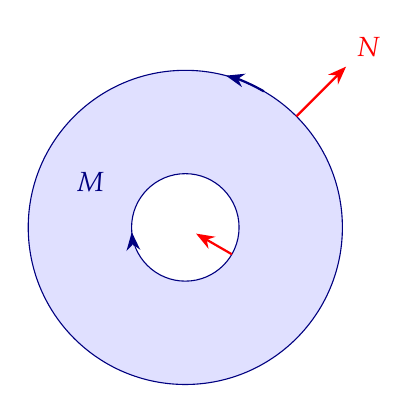
\begin{tikzpicture}[>=Stealth,scale=1.05]
  \fill[blue!12] (0,0) circle (1.9);
  \fill[white] (0,0) circle (0.65);
  \draw[navy] (0,0) circle (1.9);
  \draw[navy] (0,0) circle (0.65);
  \node[navy] at (-1.15,0.55) {$M$};
  % outer boundary: ccw arrow
  \draw[->,navy,thick] (60:1.9) arc (60:75:1.9);
  \draw[->,red,thick] (45:1.9)--(45:2.75) node[above right] {$N$};
  % inner boundary: clockwise arrow, N points into the hole
  \draw[->,navy,thick] (200:0.65) arc (200:185:0.65);
  \draw[->,red,thick] (330:0.65)--(330:0.15);
\end{tikzpicture}

\small $N=$ outward normal of $M$ (on the inner circle it points into the hole)
\caption{An annulus $M$ with its induced boundary orientation: the outer circle is traversed counter-clockwise and the inner circle clockwise, so that the region lies to the left. Applied to the angle form of Example~\ref{ex:angle} ($\dd\omega=0$) Stokes gives $\oint_{\mathrm{outer}}\omega-\oint_{\mathrm{inner\ (ccw)}}\omega=0$: both equal $2\pi$.}
\label{fig:annulus}
\end{figure}

\subsection{The structural meaning: $\dd$ is the adjoint of $\partial$}\label{sec:adjoint}

The modern reading of \eqref{eq:stokes} is obtained by introducing the pairing between $k$-forms and $k$-chains $c$ (formal sums of oriented $k$-dimensional pieces): $\langle c,\alpha\rangle:=\int_c\alpha$. Then Stokes' theorem says
\begin{equation}\label{eq:adjoint}
\langle c,\dd\alpha\rangle=\langle\partial c,\alpha\rangle,
\end{equation}
\ie the exterior derivative and the boundary operator are \emph{adjoint} to each other. Consequences:
\begin{itemize}
\item $\partial^2=0$ (the boundary of a boundary is empty) is the dual of $\dd^2=0$, and each explains the other. Indeed, applying \eqref{eq:adjoint} twice: $\langle c,\dd\dd\alpha\rangle=\langle\partial c,\dd\alpha\rangle=\langle\partial\partial c,\alpha\rangle$. If $\partial\partial c=0$ the right-hand side vanishes for every $c$, and a form whose integral over every small piece is zero must be zero: $\dd\dd\alpha=0$.
\item Integration is a chain map from the de Rham complex $(\Omega^\bullet(M),\dd)$ to the singular cochain complex, hence it descends to cohomology. de Rham's theorem (1931): this map $H^k_{\mathrm{dR}}(M)\to H^k(M;\R)$ is an isomorphism. Closed forms integrate to the same value over homologous cycles (``periods''), as in Example~\ref{ex:angle}.
\item Stokes' theorem is \emph{metric-free} and uses only a smooth structure and an orientation. Metrics enter only when we translate forms into vector fields.
\item Applications reach well beyond calculus: degree theory and the Brouwer fixed-point theorem, the Poincar\'e lemma and Poincar\'e duality, conservation laws, and Maxwell's equations $\dd F=0$, $\dd\hodge F=J$, whose integral forms are the laws of Faraday and Gauss.
\end{itemize}

\subsection{Classical corollaries}\label{sec:classical}

Let $\R^3$ carry its Euclidean metric $g$, orientation and volume form $\vol=\dd x\wedge\dd y\wedge\dd z$. With the musical isomorphisms $\flat,\sharp$ and the Hodge star $\hodge$ one has the dictionary
\[
\operatorname{grad}f=(\dd f)^\sharp,\qquad
\operatorname{curl}F=\bigl(\hodge\,\dd F^\flat\bigr)^\sharp,\qquad
\operatorname{div}F=\hodge\,\dd\hodge F^\flat,\qquad
\iota_F\vol=\hodge F^\flat .
\]
Applying Theorem~\ref{thm:stokes} to forms of degree $0,1,2$ yields:

\begin{center}
\small
\renewcommand{\arraystretch}{1.4}
\begin{tabular}{@{}p{2.5cm}p{4.5cm}p{7.0cm}@{}}
\toprule
\textbf{Form of Stokes} & \textbf{Differential forms} & \textbf{Classical statement}\\
\midrule
$n=1$ & $\int_a^b\dd f=f(b)-f(a)$ & fundamental theorem of calculus / gradient theorem\\
$n=2$ (planar $D$) & $\int_D\dd\omega=\oint_{\partial D}\omega$ & Green: $\oint P\,\dd x+Q\,\dd y=\iint(Q_x-P_y)\,\dd A$\\
$n=2$ (surface $S\subset\R^3$) & $\int_S\dd F^\flat=\oint_{\partial S}F^\flat$ & Kelvin--Stokes: $\oint F\cdot\dd r=\iint(\operatorname{curl}F)\cdot n\,\dd A$\\
$n=3$ & $\int_\Omega\dd(\iota_F\vol)=\int_{\partial\Omega}\iota_F\vol$ & Gauss: $\iiint\operatorname{div}F\,\dd V=\iint_{\partial\Omega}F\cdot n\,\dd A$\\
\bottomrule
\end{tabular}
\end{center}

\subhead{Verification of the dictionary, step by step}
In $\R^3$ with the Euclidean metric, lowering an index changes nothing numerically: $F^\flat=F_x\dd x+F_y\dd y+F_z\dd z$. Recall \eqref{eq:iotavol}: $\iota_G\vol=G_x\,\dd y\wedge\dd z+G_y\,\dd z\wedge\dd x+G_z\,\dd x\wedge\dd y$.

\emph{(i) Curl.} Compute $\dd F^\flat$ term by term, using $\dd x\wedge\dd x=0$:
\begin{align*}
\dd(F_x\dd x)&=\partial_yF_x\,\dd y\wedge\dd x+\partial_zF_x\,\dd z\wedge\dd x=-\partial_yF_x\,\dd x\wedge\dd y+\partial_zF_x\,\dd z\wedge\dd x,\\
\dd(F_y\dd y)&=\partial_xF_y\,\dd x\wedge\dd y+\partial_zF_y\,\dd z\wedge\dd y=\partial_xF_y\,\dd x\wedge\dd y-\partial_zF_y\,\dd y\wedge\dd z,\\
\dd(F_z\dd z)&=\partial_xF_z\,\dd x\wedge\dd z+\partial_yF_z\,\dd y\wedge\dd z=-\partial_xF_z\,\dd z\wedge\dd x+\partial_yF_z\,\dd y\wedge\dd z.
\end{align*}
Adding and collecting the three basis $2$-forms:
\[
\dd F^\flat=(\partial_yF_z-\partial_zF_y)\,\dd y\wedge\dd z+(\partial_zF_x-\partial_xF_z)\,\dd z\wedge\dd x+(\partial_xF_y-\partial_yF_x)\,\dd x\wedge\dd y=\iota_{\operatorname{curl}F}\vol,
\]
since the three coefficients are exactly the components of $\operatorname{curl}F$. Because $\hodge\hodge=1$ in $\R^3$ and $\hodge(\dd y\wedge\dd z)=\dd x$, etc., this is the same as $\operatorname{curl}F=(\hodge\,\dd F^\flat)^\sharp$.

\emph{(ii) Divergence.} $\iota_F\vol=F_x\dd y\wedge\dd z+F_y\dd z\wedge\dd x+F_z\dd x\wedge\dd y$. Differentiating, only the derivative with respect to the variable missing from each $2$-form survives:
$\dd(F_x\dd y\wedge\dd z)=\partial_xF_x\,\dd x\wedge\dd y\wedge\dd z$, $\dd(F_y\dd z\wedge\dd x)=\partial_yF_y\,\dd y\wedge\dd z\wedge\dd x$, $\dd(F_z\dd x\wedge\dd y)=\partial_zF_z\,\dd z\wedge\dd x\wedge\dd y$,
and the three $3$-forms equal $\dd x\wedge\dd y\wedge\dd z$ (cyclic permutations of three $1$-forms are even). So $\dd(\iota_F\vol)=(\operatorname{div}F)\,\vol$.

\emph{(iii) Kelvin--Stokes.} For an oriented surface $S\subset\R^3$ with unit normal $n$ the restriction satisfies $\iota_G\vol|_S=\langle G,n\rangle\,\dd A$ (same computation as in Lemma~\ref{lem:fluxbdry} below, with $e_1=n$ and $e_2,e_3$ tangent to $S$). Then
\[
\oint_{\partial S}F\cdot\dd r=\oint_{\partial S}F^\flat\overset{\text{Stokes}}=\int_S\dd F^\flat=\int_S\iota_{\operatorname{curl}F}\vol=\iint_S\langle\operatorname{curl}F,n\rangle\,\dd A .
\]
\emph{(iv) Gauss.} $\displaystyle\int_\Omega(\operatorname{div}F)\,\dd V\overset{\text{(ii)}}=\int_\Omega\dd(\iota_F\vol)\overset{\text{Stokes}}=\int_{\partial\Omega}\iota_F\vol=\iint_{\partial\Omega}\langle F,n\rangle\,\dd A$, again by the restriction formula.

% =====================================================================
\section{The Gauss (divergence) theorem}\label{sec:gauss}
% =====================================================================

\subsection{Divergence is defined by a volume form, not by a metric}\label{sec:divmu}

Let $\mu$ be a nowhere-vanishing $n$-form on $M$ (a \emph{volume form}; in the Riemannian case $\mu=\vol_g=\sqrt{|g|}\,\dd x^1\wedge\cdots\wedge\dd x^n$). The \emph{divergence} of a vector field $X$ is defined by
\begin{equation}\label{eq:Lmu}
\Lie_X\mu=(\operatorname{div}_\mu X)\,\mu,
\end{equation}
that is, as the relative rate of change of volume under the flow of $X$. Since $\dd\mu=0$ (it is an $(n+1)$-form), Cartan's formula \eqref{eq:cartan} gives
\begin{equation}\label{eq:divmu}
\dd(\iota_X\mu)=\Lie_X\mu=(\operatorname{div}_\mu X)\,\mu .
\end{equation}
\emph{Coordinate formula, step by step.} Let $\mu=\sqrt{|g|}\,\dd x^1\wedge\cdots\wedge\dd x^n$ and $X=X^i\partial_i$.
\begin{enumerate}
\item Contract (antiderivation rule applied repeatedly, as in Section~\ref{sec:flux}): \[\iota_X\mu=\sqrt{|g|}\sum_i(-1)^{i-1}X^i\,\dd x^1\wedge\cdots\wedge\widehat{\dd x^i}\wedge\cdots\wedge\dd x^n.\]
\item Differentiate: in $\dd(\sqrt{|g|}X^i)\wedge\dd x^1\wedge\cdots\wedge\widehat{\dd x^i}\wedge\cdots$ only $\partial_i(\sqrt{|g|}X^i)\,\dd x^i$ survives (the other $\dd x^j$ are repeated), and moving $\dd x^i$ to its place gives another $(-1)^{i-1}$. The two signs cancel: $\dd(\iota_X\mu)=\sum_i\partial_i(\sqrt{|g|}X^i)\,\dd x^1\wedge\cdots\wedge\dd x^n$.
\item Divide by $\mu$:
\begin{equation}\label{eq:divcoord}
\operatorname{div}_\mu X=\frac1{\sqrt{|g|}}\,\partial_i\bigl(\sqrt{|g|}\,X^i\bigr),
\end{equation}
which reduces to $\partial_iX^i$ in Cartesian coordinates ($|g|=1$).
\end{enumerate}
So the divergence theorem is nothing but Theorem~\ref{thm:stokes} applied to the $(n-1)$-form $\omega=\iota_X\mu$ obtained from $X$ by (partial) contraction.

\subsection{The boundary term: from $\iota_X\mu$ to $\langle X,N\rangle\,\dd A$}\label{sec:boundaryterm}

\begin{lemma}\label{lem:fluxbdry}
Let $(M,g)$ be an oriented Riemannian manifold with boundary, $N$ the outward unit normal and $\dd A$ the Riemannian area form of $\partial M$ (with the induced orientation). Then
\[
j\pb\bigl(\iota_X\vol_g\bigr)=\langle X,N\rangle\,\dd A .
\]
\end{lemma}
\begin{proof}
\Step{1}{adapted frame} At a boundary point choose an oriented orthonormal frame $e_1=N,e_2,\dots,e_n$ ($e_2,\dots,e_n$ tangent to $\partial M$) with dual coframe $e^1,\dots,e^n$. Then $\vol_g=e^1\wedge\cdots\wedge e^n$. By the induced-orientation convention $(e_2,\dots,e_n)$ is a positive orthonormal basis of $T\partial M$, so $\dd A=j\pb(e^2\wedge\cdots\wedge e^n)$.
\Step{2}{contract} Apply $\iota_X$ one factor at a time: $\iota_X(e^i\wedge\beta)=X^i\beta-e^i\wedge\iota_X\beta$. For $n=3$:
\begin{align*}
\iota_X(e^1\wedge e^2\wedge e^3)&=X^1e^2\wedge e^3-e^1\wedge\iota_X(e^2\wedge e^3)\\
&=X^1e^2\wedge e^3-e^1\wedge(X^2e^3-X^3e^2)=X^1e^2\wedge e^3-X^2e^1\wedge e^3+X^3e^1\wedge e^2 .
\end{align*}
In general, $\iota_X\vol_g=\sum_{i=1}^n(-1)^{i-1}X^i\,e^1\wedge\cdots\wedge\widehat{e^i}\wedge\cdots\wedge e^n$.
\Step{3}{restrict to $\partial M$} The covector $e^1=\langle N,\cdot\rangle$ vanishes on all tangent vectors $e_2,\dots,e_n$, so $j\pb e^1=0$ and every term containing $e^1$ (all $i\ne1$) restricts to zero. Only $i=1$ survives: $j\pb(\iota_X\vol_g)=X^1j\pb(e^2\wedge\cdots\wedge e^n)=X^1\dd A$, and $X^1=\langle X,e_1\rangle=\langle X,N\rangle$. In the $n=3$ example above this reads $j\pb(\cdots)=X^1e^2\wedge e^3$.
\end{proof}

\subsection{Statement and proof}

\begin{theorem}[Gauss--Ostrogradsky, divergence theorem]\label{thm:gauss}
Let $(M,g)$ be a compact oriented Riemannian $n$-manifold with boundary and $X$ a smooth vector field. Then
\[
\int_M\operatorname{div}X\,\dd V=\int_{\partial M}\langle X,N\rangle\,\dd A .
\]
\end{theorem}
\begin{proof}
By \eqref{eq:divmu}, $\operatorname{div}X\,\vol_g=\dd(\iota_X\vol_g)$. Apply Theorem~\ref{thm:stokes} to $\omega=\iota_X\vol_g$ and use Lemma~\ref{lem:fluxbdry}.
\end{proof}

\begin{example}[The position field on the unit ball]\label{ex:ball}
Let $X=x\partial_x+y\partial_y+z\partial_z$ on the unit ball $B\subset\R^3$.
\begin{enumerate}
\item \emph{Volume side.} $\operatorname{div}X=\partial_xx+\partial_yy+\partial_zz=3$, so $\int_B3\,\dd V=3\cdot\frac{4\pi}3=4\pi$.
\item \emph{Boundary side, with the formula of the lemma.} On the unit sphere the outward normal is $N=(x,y,z)=X$, hence $\langle X,N\rangle=x^2+y^2+z^2=1$, and the flux is $\int_{S^2}1\,\dd A=4\pi$.
\item \emph{Boundary side, directly with forms.} $\iota_X\vol=x\,\dd y\wedge\dd z+y\,\dd z\wedge\dd x+z\,\dd x\wedge\dd y$ (formula \eqref{eq:iotavol}). At the north pole $(0,0,1)$ the tangent plane is spanned by $\partial_x,\partial_y$, where $\dd z=0$, so the restriction is $z\,\dd x\wedge\dd y=\dd x\wedge\dd y=\dd A$, again with coefficient $1$.
\end{enumerate}
Both sides equal $4\pi$ \checkmark.
\end{example}

\begin{synthesis}[the area form of the sphere is a contraction]\label{syn:sphere}
In Section~\ref{sec:tensorfields} the area form of the sphere of radius $r$ was defined by $\alpha_p(v_1,v_2)=\frac1r(v_1\times v_2)\cdot p$. Since $(v_1\times v_2)\cdot N=\vol(N,v_1,v_2)$ for $N=p/r$ (triple product),
$\alpha=\iota_N\vol$ restricted to the sphere: this is Lemma~\ref{lem:fluxbdry} with $X=N$, $\langle N,N\rangle=1$. In spherical coordinates it is $r^2\sin\theta\,\dd\theta\wedge\dd\varphi$, with total area $4\pi r^2$, and Example~\ref{ex:ball} (flux of the position field through $S^2$, $=4\pi$) is the case $r=1$.
\end{synthesis}

\begin{remark}[What needs what]\label{rem:whatneeds}
\begin{itemize}
\item \emph{Stokes:} smooth structure $+$ orientation only. No metric, no volume.
\item \emph{Divergence/Gauss:} Stokes $+$ a volume form $\mu$ to turn a vector field into an $(n-1)$-form via $\iota_X\mu$. A metric is needed only to rewrite the flux as $\langle X,N\rangle\,\dd A$. On non-orientable manifolds the theorem survives if $\mu$ is a density.
\item \emph{Kelvin--Stokes / curl:} orientation, a metric and dimension $3$, since the identification of $2$-forms with vector fields ($\hodge$) is special to $n=3$. In other dimensions the object is $\dd\omega$, not a ``curl vector''.
\end{itemize}
\end{remark}

\begin{keypoints}[Part III]
\begin{itemize}
\item $\int_\gamma\omega=\int\langle\omega,\dot\gamma\rangle\,\dd t$: integration of a $1$-form is contraction with the velocity; $\int_\phi\alpha$ is full contraction with the tangent $k$-frame.
\item Stokes: $\int_M\dd\omega=\int_{\partial M}\omega$, equivalently $\langle c,\dd\alpha\rangle=\langle\partial c,\alpha\rangle$. Metric-free.
\item Gauss is Stokes for $\omega=\iota_X\mu$ with $\dd\iota_X\mu=\Lie_X\mu=\operatorname{div}_\mu X\,\mu$.
\end{itemize}
\end{keypoints}


\clearpage
% =====================================================================
\part{Connections, geodesics and curvature}\label{part:geometry}
% =====================================================================

Part~\ref{part:integration} needed only a smooth structure and an orientation. To differentiate \emph{vectors} we must compare tangent spaces at nearby points, and
that requires extra structure: a \emph{connection}. A metric singles out one canonical connection (Levi-Civita), whose geodesics are the straightest curves, and
whose failure to be ``flat'' is the Riemann curvature tensor: the mathematical content of gravity in general relativity.

% =====================================================================
\section{Connections and the covariant derivative}\label{sec:conn}
% =====================================================================
% ---- begin extract GR lines 610-743 ----
\subsection{Definition}
\begin{intuition}[{derivative = ``compare with the parallel copy''}]
We choose a rule that says what it means for a vector to be ``kept constant'' while we move along a curve: this is \textbf{parallel transport} $\Pi$. Then the derivative of a vector field $Y$ along $X$ is the limit of $\frac1\varepsilon\big(\Pi^{-1}(Y_{\phi_\varepsilon(p)})-Y_p\big)$: how much $Y$ differs from the parallel copy of itself. Infinitesimally, the same information is encoded algebraically by a \emph{connection} $\nabla$. This is the analogue of the relation between a vector field $X$ (infinitesimal) and its flow $\phi$ (finite).
\end{intuition}
\begin{formal}[{connection (affine connection)}]
A \emph{connection} on $M$ is a map $\Xfield(M)\times\Xfield(M)\to\Xfield(M)$, $(X,Y)\mapsto\nabla_XY$ such that
\begin{enumerate}[label=(\roman*),nosep]
\item it is $\R$-bilinear;
\item $\nabla_{fX}Y=f\,\nabla_XY$ for $f\in C^\infty(M)$ ($C^\infty$-linear in the direction $X$: only $X_p$ matters);
\item $\nabla_X(fY)=X(f)\,Y+f\,\nabla_XY$ (Leibniz/product rule in $Y$).
\end{enumerate}
In a chart the \emph{Christoffel symbols} $\Gamma^k{}_{ij}(x)$ are defined by
\[
\nabla_{\partial_i}\partial_j=\Gamma^k{}_{ij}\,\partial_k ,
\]
and then for $X=X^i\partial_i$, $Y=Y^j\partial_j$:
\begin{equation}\label{eq:covdev}
\nabla_XY=X^i\Big(\frac{\partial Y^k}{\partial x^i}+\Gamma^k{}_{ij}Y^j\Big)\partial_k .
\end{equation}
Given $\Gamma^k{}_{ij}$ in one chart, $\nabla$ is completely determined there. Conversely any choice of smooth functions $\Gamma^k{}_{ij}$ defines a connection on the chart domain.
\end{formal}
\begin{intuition}[{Christoffel symbols = correction terms}]
$\partial_iY^k$ is the change of the \emph{components} of $Y$; $\Gamma^k{}_{ij}Y^j$ is the correction due to the fact that the \emph{basis vectors} themselves change from point to point (if you walk along a circle, the basis $\partial_r,\partial_\varphi$ rotates). Even a constant vector field $Y=\mathrm{const}$ in the plane has $\partial_iY^k\neq0$ in polar coordinates; the $\Gamma$ term compensates exactly.
\end{intuition}

\begin{formal}[{$\Gamma$ is not a tensor}]
Under a coordinate change $x\mapsto\tilde x$,
\begin{equation}\label{eq:christtransf}
\tilde\Gamma^{\tilde k}{}_{\tilde i\tilde j}=\frac{\partial x^i}{\partial\tilde x^{\tilde i}}\frac{\partial x^j}{\partial\tilde x^{\tilde j}}\,\Gamma^k{}_{ij}\,\frac{\partial\tilde x^{\tilde k}}{\partial x^k}\;+\;\frac{\partial^2x^k}{\partial\tilde x^{\tilde i}\partial\tilde x^{\tilde j}}\frac{\partial\tilde x^{\tilde k}}{\partial x^k}.
\end{equation}
The first term is the tensor rule \eqref{eq:tensortransf}; the second is the extra term that spoils tensoriality. (Consequence: $\Gamma$ can vanish in one chart and not in another, as below.) The two connections $\nabla^0,\nabla^1$ differ by a genuine tensor, so connections form an affine space.
\end{formal}

\begin{example}[{Christoffel symbols of the Euclidean connection in polar coordinates}]
Let $\nabla^0$ be the connection with $\Gamma=0$ in Cartesian coordinates $(x,y)$ (\ie $\nabla^0_X\partial_x=\nabla^0_X\partial_y=0$). In the formula \eqref{eq:christtransf} only the second term survives:
$\tilde\Gamma^{\tilde k}{}_{\tilde i\tilde j}=\frac{\partial^2x^l}{\partial\tilde x^{\tilde i}\partial\tilde x^{\tilde j}}\frac{\partial\tilde x^{\tilde k}}{\partial x^l}$, with $x=r\cos\varphi$, $y=r\sin\varphi$, $\partial_xr=\cos\varphi$, $\partial_yr=\sin\varphi$, $\partial_x\varphi=-\sin\varphi/r$, $\partial_y\varphi=\cos\varphi/r$:
\begin{align*}
\Gamma^r{}_{\varphi\varphi}&=(-r\cos\varphi)(\cos\varphi)+(-r\sin\varphi)(\sin\varphi)=-r,\\
\Gamma^\varphi{}_{r\varphi}=\Gamma^\varphi{}_{\varphi r}&=(-\sin\varphi)\Big(\tfrac{-\sin\varphi}{r}\Big)+(\cos\varphi)\Big(\tfrac{\cos\varphi}{r}\Big)=\tfrac1r,
\end{align*}
and all the others vanish ($\Gamma^r{}_{rr}=\Gamma^r{}_{r\varphi}=\Gamma^\varphi{}_{rr}=\Gamma^\varphi{}_{\varphi\varphi}=0$). \checkmark\ Interpretation: $\nabla_{\partial_\varphi}\partial_\varphi=-r\,\partial_r$ (the basis vector $\partial_\varphi$ turns inwards as you go around) and $\nabla_{\partial_r}\partial_\varphi=\frac1r\partial_\varphi$ ($\partial_\varphi$ grows linearly with $r$).
\end{example}

\begin{example}[{a connection is extra structure: the ``cylindrical'' connection}]
On $\R^2\setminus\{0\}$ define $\nabla^1$ by declaring $\Gamma=0$ in the \emph{polar} chart, \ie $\nabla^1_{\partial_a}\partial_b=0$ for $a,b\in\{r,\varphi\}$. This is a perfectly good connection, but \textbf{different} from $\nabla^0$ (since $\Gamma^r{}_{\varphi\varphi}=-r\neq0$ for $\nabla^0$). Differences: $\nabla^1$ keeps $\partial_r,\partial_\varphi$ ``constant'' (so arrows rotate with the polar frame) while $\nabla^0$ keeps $\partial_x,\partial_y$ constant. Their geodesics differ: for $\nabla^1$ geodesics satisfy $\ddot r=\ddot\varphi=0$ (spirals $r=r_0+at$, $\varphi=\varphi_0+bt$), for $\nabla^0$ they are straight lines.
\end{example}

\subsection{Covariant derivative of covectors and general tensors}
\begin{formal}[{extension to all tensors}]
There is a unique extension of $\nabla_X$ to $\TF{\ell}{k}(M)$ (still of the same type) such that
\begin{itemize}[nosep]
\item $\nabla_Xf=X(f)$ for functions;
\item $\nabla_X(\tau_1\otimes\tau_2)=\nabla_X\tau_1\otimes\tau_2+\tau_1\otimes\nabla_X\tau_2$;
\item it commutes with contractions, equivalently
$\nabla_X\big(\tau(v_1,\dots,v_k,\alpha_1,\dots,\alpha_\ell)\big)=(\nabla_X\tau)(\dots)+\sum_i\tau(\dots,\nabla_Xv_i,\dots)+\sum_j\tau(\dots,\nabla_X\alpha_j,\dots)$.
\end{itemize}
For a 1-form $(\nabla_X\omega)(Y)=X(\omega(Y))-\omega(\nabla_XY)$. In coordinates (\emph{semicolon / index notation}, with the derivative index first):
\begin{align*}
\nabla_iV^k&=\partial_iV^k+\Gamma^k{}_{ij}V^j,\\
\nabla_i\omega_j&=\partial_i\omega_j-\Gamma^k{}_{ij}\omega_k,\\
\nabla_r T^{a}{}_{b}&=\partial_rT^a{}_b+\Gamma^a{}_{rs}T^s{}_b-\Gamma^s{}_{rb}T^a{}_s .
\end{align*}
Rule of thumb: every upper index gets a $+\Gamma$ term and every lower index a $-\Gamma$ term. The result $\nabla\tau$ is a tensor of type $(\ell,k+1)$ with components $\tau^{\dots}{}_{\dots;r}=\nabla_r\tau^{\dots}{}_{\dots}$ even though $\partial_r\tau$ and $\Gamma$ are not tensors separately: the non-tensorial parts cancel.
\end{formal}
\begin{intuition}[{covectors are the ``dual'' behaviour}]
Since $\omega(Y)$ must obey the ordinary product rule for a scalar, $\nabla$ on covectors \emph{must} compensate the connection acting on vectors; this forces the minus sign.
\end{intuition}

\begin{example}[{divergence in polar coordinates}]
For a vector field $V$, $\mathrm{div}\,V:=\nabla_iV^i=\partial_iV^i+\Gamma^i{}_{ij}V^j$. With the polar $\Gamma$: $\Gamma^i{}_{ir}=\Gamma^r{}_{rr}+\Gamma^\varphi{}_{\varphi r}=\frac1r$ and $\Gamma^i{}_{i\varphi}=0$, therefore
\[
\mathrm{div}\,V=\partial_rV^r+\partial_\varphi V^\varphi+\frac{V^r}{r}=\frac1r\partial_r(rV^r)+\partial_\varphi V^\varphi ,
\]
the familiar formula (with $V^\varphi$ the component on $\partial_\varphi$). No ad-hoc ``scale factors'' were needed: they are all contained in $\Gamma$.
\end{example}

\subsection{Parallel transport}
\begin{formal}[{parallel transport along a curve}]
For a smooth curve $\gamma(t)$ and a vector field $Y$ along $\gamma$ (a smooth assignment $t\mapsto Y_{\gamma(t)}\in T_{\gamma(t)}M$), define $\nabla_{\dot\gamma}Y:=\nabla_{\hat X}\hat Y$ for any extensions $\hat X,\hat Y$ of $\dot\gamma, Y$ to fields on $M$; the result does not depend on the extensions. In coordinates $\gamma=(x^i(t))$:
\[
(\nabla_{\dot\gamma}Y)^k=\frac{\dd Y^k}{\dd t}+\Gamma^k{}_{ij}(\gamma(t))\,\dot x^i\,Y^j .
\]
\textbf{Theorem.} Given $v_0\in T_{\gamma(t_0)}M$ there is a unique field $Y$ along $\gamma$ with $Y_{\gamma(t_0)}=v_0$ and $\nabla_{\dot\gamma}Y=0$. (In coordinates this is the linear ODE
\begin{equation}\label{eq:ptode}
\frac{\dd Y^k}{\dd t}+\Gamma^k{}_{ij}(\gamma(t))\,\dot x^i\,Y^j=0,
\end{equation}
so existence and uniqueness follow from ODE theory; a general curve is split into finitely many chart pieces.) The \emph{parallel transport} is the linear isomorphism $\Pi^\gamma_{\gamma(t_0),\gamma(t_1)}:T_{\gamma(t_0)}M\to T_{\gamma(t_1)}M$, $v_0\mapsto Y_{\gamma(t_1)}$.
\end{formal}
\begin{intuition}[{carrying an arrow without turning it}]
Like carrying a spear while walking and trying not to rotate it ``relative to the ground''. On a curved surface this is ambiguous globally, but infinitesimally it is perfectly well defined by \eqref{eq:ptode}. In a flat space with $\nabla^0$ and Cartesian coordinates ($\Gamma=0$) parallel transport leaves components unchanged ($\Pi(v_0)=v_0$ via $T_p\R^m\cong\R^m$).
\end{intuition}

\begin{example}[{parallel transport on the sphere: path-dependence}]
For the unit sphere (metric $\dd\theta^2+\sin^2\theta\,\dd\phi^2$; Christoffel symbols computed in Section~\ref{sec:lc}): $\Gamma^\theta{}_{\phi\phi}=-\sin\theta\cos\theta$, $\Gamma^\phi{}_{\theta\phi}=\cot\theta$. 
\emph{Along the equator} $\theta=\pi/2$, $\dot\theta=0$, $\dot\phi=1$: both symbols vanish at $\theta=\pi/2$, so \eqref{eq:ptode} gives $\dot Y^\theta=\dot Y^\phi=0$: the components $(Y^\theta,Y^\phi)$ stay constant.
\emph{Along a meridian} ($\phi=\mathrm{const}$, $\dot\theta=1$): $\dot Y^\theta=0$ and $\dot Y^\phi+\cot\theta\,Y^\phi=0$, so $Y^\theta$ is constant, $Y^\phi\propto 1/\sin\theta$ (hence its length $\sin\theta\,|Y^\phi|$ is constant).
\emph{A triangle.} Go from the north pole down the meridian $\phi=0$ to the equator, along the equator to $\phi=\pi/2$, and back up to the pole. Start at the pole with a vector pointing along the first meridian's direction ``away from the pole'' ($\theta$-direction at $\phi=0$). Transported down the first meridian it remains tangent to it; along the equator it stays pointing towards the south (constant $Y^\theta$), perpendicular to the path; going back up the second meridian it remains the same way, now pointing \emph{along} the second meridian, away from the pole. At the end the vector has rotated by $\pi/2$ with respect to the initial one. The rotation angle equals the enclosed area times the curvature ($K=1$): the octant has area $4\pi/8=\pi/2$. \textbf{Parallel transport depends on the path precisely because the space is curved} (Section~\ref{sec:curv}).
\end{example}

\subsection{Geodesics}
\begin{formal}[{geodesic}]
A curve $\gamma(t)$ is a \emph{geodesic} of $\nabla$ if $\nabla_{\dot\gamma}\dot\gamma=0$ for all $t$ (it parallel-transports its own tangent vector: ``auto-parallelism''). In coordinates:
\begin{equation}\label{eq:geodesic}
\ddot x^k+\Gamma^k{}_{ij}(x(t))\,\dot x^i\dot x^j=0 .
\end{equation}
This is a second-order ODE: given a point and an initial velocity there is a unique maximal geodesic. If one reparametrizes, $\gamma(t)=\rho(s(t))$, then $\gamma$ is a geodesic as a set iff $\rho$ satisfies $\frac{\dd^2y^k}{\dd s^2}+\Gamma^k{}_{ij}\frac{\dd y^i}{\dd s}\frac{\dd y^j}{\dd s}=f(s)\frac{\dd y^k}{\dd s}$ with $f=-s''/(s')^2$; geodesics with $f=0$ are called \emph{affinely parametrized} (and \eqref{eq:geodesic} is that case).
\end{formal}
\begin{intuition}[{the straightest possible path; free fall}]
A geodesic is a curve with zero covariant acceleration: ``no one pushes me, I just follow the geometry''. In $\R^m$ with $\nabla^0$ it is $\ddot x=0$: uniform straight motion. The term $-\Gamma^k{}_{ij}\dot x^i\dot x^j$ is the acceleration that \emph{coordinates} see; in GR it is precisely what we call the ``gravitational force'' (and in polar coordinates, the ``centrifugal'' force). In GR: \textbf{freely falling particles move along timelike geodesics; light along null geodesics.}
\end{intuition}

\begin{example}[{straight lines in polar coordinates $\Rightarrow$ centrifugal force}]
With $\Gamma^r{}_{\varphi\varphi}=-r$, $\Gamma^\varphi{}_{r\varphi}=1/r$, equation \eqref{eq:geodesic} reads
\[
\ddot r-r\dot\varphi^2=0,\qquad \ddot\varphi+\frac2r\dot r\dot\varphi=0 .
\]
The second equation gives $\frac{\dd}{\dd t}(r^2\dot\varphi)=r(\,r\ddot\varphi+2\dot r\dot\varphi)=0$: $L=r^2\dot\varphi$ is conserved (angular momentum). Then $\ddot r=L^2/r^3$: a repulsive ``centrifugal'' term appears even though nothing is pushing the particle; it is just a straight line seen in a rotating-frame-like coordinate system. \emph{Check with the line $x=d$, $y=vt$:} $r^2=d^2+v^2t^2$, $\varphi=\arctan(vt/d)$, so $r^2\dot\varphi=vd$ is constant, and $\ddot r=v^2d^2/r^3=L^2/r^3$ with $L=vd$. \checkmark
\end{example}

\begin{example}[{geodesic equations on the unit sphere}]
Using $\Gamma^\theta{}_{\phi\phi}=-\sin\theta\cos\theta$, $\Gamma^\phi{}_{\theta\phi}=\cot\theta$:
\[
\ddot\theta-\sin\theta\cos\theta\,\dot\phi^2=0,\qquad\ddot\phi+2\cot\theta\,\dot\theta\dot\phi=0 .
\]
\textit{Equator} $\theta=\pi/2$, $\dot\theta=0$: both equations hold for $\phi=\omega t$ $\Rightarrow$ the equator is a geodesic (a great circle). \textit{Circle of latitude} $\theta=\theta_0\neq\pi/2$, $\phi=\omega t$: the first equation gives $\ddot\theta=\sin\theta_0\cos\theta_0\,\omega^2\neq0$, contradicting $\ddot\theta=0$ $\Rightarrow$ it is \textbf{not} a geodesic: you must push to stay on it. All geodesics of the sphere are great circles.
\end{example}

\begin{exercises}
\begin{enumerate}[nosep]
\item Verify from \eqref{eq:christtransf} that $\tilde\Gamma^{\tilde k}{}_{\tilde i\tilde j}$ is symmetric in its lower indices if $\Gamma$ is.
\item Write $\nabla_X(f\omega)=X(f)\omega+f\nabla_X\omega$ and check it in coordinates.
\item Show that the geodesic equation implies that $g(\dot\gamma,\dot\gamma)$ is constant when $\nabla$ is the Levi-Civita connection (next section).
\end{enumerate}
\end{exercises}
%% ---- end extract ----


% =====================================================================
\section{Torsion, the Levi-Civita connection and geodesics}\label{sec:lc}
% =====================================================================
% ---- begin extract GR lines 747-830 ----

\begin{formal}[{torsion}]
The \emph{torsion} of $\nabla$ is $\mathrm{Tor}(X,Y)=\nabla_XY-\nabla_YX-[X,Y]$. It is $C^\infty(M)$-linear in both arguments, hence given by a tensor $T\in\TF{1}{2}(M)$; in a chart $T^i{}_{jk}=\Gamma^i{}_{jk}-\Gamma^i{}_{kj}$. It is antisymmetric: $T(X,Y)=-T(Y,X)$. The connection is called \emph{symmetric} (or \emph{torsion-free}) if $T=0$, which in coordinates means $\Gamma^i{}_{jk}=\Gamma^i{}_{kj}$.
\end{formal}
\begin{intuition}[{torsion = twisting of the frames}]
Torsion measures whether an infinitesimal parallelogram built by parallel-transporting two small vectors along each other closes up. Torsion-free means ``no screw-like twisting''. In GR we always assume $T=0$.
\end{intuition}

\begin{formal}[{metric compatibility and the Levi-Civita theorem}]
Let $g$ be a metric. A connection is \emph{metric} if $\nabla_Xg=0$ for all $X$, \ie $X\big(g(Y,Z)\big)=g(\nabla_XY,Z)+g(Y,\nabla_XZ)$.

\textbf{Theorem (Fundamental theorem of (pseudo-)Riemannian geometry).} For every metric $g$ there is a \emph{unique} connection $\nabla=\nabla^{LC}$ that is (i) metric and (ii) torsion-free. It is determined by the \emph{Koszul formula}
\begin{align*}
2g(\nabla_XY,Z)&=X\big(g(Y,Z)\big)+Y\big(g(X,Z)\big)-Z\big(g(X,Y)\big)\\
&\quad+g([Z,X],Y)+g([X,Y],Z)-g(X,[Y,Z]).
\end{align*}
\emph{Idea of the proof.} Write the metric property for $(X;Y,Z)$, $(Y;Z,X)$, $(Z;X,Y)$, add the first two and subtract the third, and use $\nabla_XY-\nabla_YX=[X,Y]$ to eliminate all covariant derivatives except $g(\nabla_XY,Z)$. Non-degeneracy of $g$ then determines $\nabla_XY$.

In coordinates, taking $X=\partial_i,Y=\partial_j,Z=\partial_l$ (all brackets vanish):
\begin{equation}\label{eq:christmetric}
\boxed{\ \Gamma^k{}_{ij}=\tfrac12\,g^{kl}\big(\partial_ig_{jl}+\partial_jg_{il}-\partial_lg_{ij}\big)\ }
\end{equation}
with $(g^{kl})$ the inverse matrix of $(g_{ij})$.
\end{formal}
\begin{intuition}[{the ``natural'' connection of a metric}]
The Levi-Civita connection is the unique way of doing parallel transport such that (i) \textbf{lengths and angles are preserved}, since $g(\Pi v,\Pi w)=g(v,w)$ and (ii) there is \textbf{no torsion}. It is therefore a function of the metric alone, $g\mapsto\nabla^{LC}$: every construction from $\nabla^{LC}$ is a construction from $g$. Geodesics of $\nabla^{LC}$ are called ``geodesics of $g$''. Also, $\nabla$ commutes with raising and lowering of indices.
\end{intuition}

\begin{example}[{Christoffel symbols from the metric}]
\textbf{Polar plane:} $g_{rr}=1,\ g_{\varphi\varphi}=r^2$. The only non-zero derivative is $\partial_rg_{\varphi\varphi}=2r$. From \eqref{eq:christmetric}: $\Gamma^r{}_{\varphi\varphi}=\frac12g^{rr}(-\partial_rg_{\varphi\varphi})=-r$, $\Gamma^\varphi{}_{r\varphi}=\frac12g^{\varphi\varphi}\partial_rg_{\varphi\varphi}=\frac1r$. \checkmark\ (The same as before: the Euclidean connection \emph{is} the Levi-Civita connection of the Euclidean metric.)

\textbf{Unit sphere:} $g_{\theta\theta}=1$, $g_{\phi\phi}=\sin^2\theta$, $\partial_\theta g_{\phi\phi}=2\sin\theta\cos\theta$:
\[
\Gamma^\theta{}_{\phi\phi}=-\tfrac12\partial_\theta g_{\phi\phi}=-\sin\theta\cos\theta,\qquad
\Gamma^\phi{}_{\theta\phi}=\Gamma^\phi{}_{\phi\theta}=\tfrac12\frac{1}{\sin^2\theta}\,\partial_\theta g_{\phi\phi}=\cot\theta,
\]
all others zero. Radius $a$ gives the same symbols (a constant rescaling of $g$ does not change $\Gamma$).

\textbf{Expanding universe (1+1 dimensions):} $g=-\dd t\otimes\dd t+a(t)^2\,\dd x\otimes\dd x$. Then $\Gamma^t{}_{xx}=\tfrac12g^{tt}(-\partial_tg_{xx})=\tfrac12(-1)(-2a\dot a)=a\dot a$, $\Gamma^x{}_{tx}=\tfrac12g^{xx}\partial_tg_{xx}=\dot a/a$.
\end{example}

\subsection{Geodesics as extremals of length (variational principle)}
\begin{formal}[{geodesics extremize the energy functional}]
For a curve $\gamma:[t_0,t_1]\to M$ consider
\[
S_1[\gamma]=\int_{t_0}^{t_1}\sqrt{g(\dot\gamma,\dot\gamma)}\,\dd t\quad(\text{arc length}),\qquad
S_2[\gamma]=\int_{t_0}^{t_1}g(\dot\gamma,\dot\gamma)\,\dd t\quad(\text{``energy''}).
\]
$\gamma$ is a critical point of $S_1$ iff (after a reparametrization) it is a critical point of $S_2$; and \textbf{$\gamma$ is a critical point of $S_2$ with fixed endpoints iff it is a geodesic of $g$}. Proof via the Euler--Lagrange equations for $\mathcal L=\tfrac12g_{ij}(x)\dot x^i\dot x^j$:
\[
\frac{\dd}{\dd t}\frac{\partial\mathcal L}{\partial\dot x^l}-\frac{\partial\mathcal L}{\partial x^l}=0\iff g_{lj}\ddot x^j+\partial_kg_{lj}\dot x^k\dot x^j-\tfrac12\partial_lg_{ij}\dot x^i\dot x^j=0,
\]
and multiplying by $g^{ml}$ and symmetrizing the middle term in $(k,j)$ gives exactly $\ddot x^m+\Gamma^m{}_{ij}\dot x^i\dot x^j=0$ with $\Gamma$ from \eqref{eq:christmetric}.
\end{formal}
\begin{intuition}[{shortest path (Riemannian), longest proper time (Lorentzian)}]
On a sphere the shortest path between two points is an arc of a great circle (not unique for antipodal points). In Minkowski space, a straight timelike worldline \emph{maximizes} the proper time between two events (twin paradox). The variational point of view is also the starting point of the Lagrangian formulation of GR and the reason why geodesic motion is a ``principle of least action''.
\end{intuition}

\begin{example}[{Euler--Lagrange in polar coordinates}]
$\mathcal L=\tfrac12(\dot r^2+r^2\dot\varphi^2)$. $\frac{\dd}{\dd t}\partial_{\dot r}\mathcal L=\ddot r$, $\partial_r\mathcal L=r\dot\varphi^2$, hence $\ddot r=r\dot\varphi^2$; and $\frac{\dd}{\dd t}(r^2\dot\varphi)=0$. These are exactly the geodesic equations above, obtained without computing a single Christoffel symbol. This is often the fastest way to find $\Gamma$: read them off as the coefficients of $-\dot x^i\dot x^j$ in the E--L equations.
\end{example}

\begin{formal}[{conserved quantities}]
If $\xi$ is a Killing field of $g$ and $\gamma$ is a geodesic then $g(\xi,\dot\gamma)$ is constant along $\gamma$. (Proof: $\frac{\dd}{\dd t}g(\xi,\dot\gamma)=g(\nabla_{\dot\gamma}\xi,\dot\gamma)+g(\xi,\nabla_{\dot\gamma}\dot\gamma)=\nabla_{(i}\xi_{j)}\dot\gamma^i\dot\gamma^j+0=0$, because $\Lie_\xi g_{ij}=\nabla_i\xi_j+\nabla_j\xi_i=0$.)
\end{formal}
\begin{example}[{conservation of angular momentum}]
$\xi=\partial_\varphi$ is Killing for $g=\dd r^2+r^2\dd\varphi^2$. Then $g(\xi,\dot\gamma)=r^2\dot\varphi$ is conserved, as we found. For Schwarzschild one gets the energy $E=-g(\partial_t,\dot\gamma)$ and $L=g(\partial_\varphi,\dot\gamma)$.
\end{example}

\begin{example}[{geodesics of an expanding universe: cosmological redshift (1+1 model)}]
From $\Gamma^t{}_{xx}=a\dot a$, $\Gamma^x{}_{tx}=\dot a/a$ (previous example), with affine parameter $\lambda$:
\[
\ddot t+a\dot a\,\dot x^2=0,\qquad\ddot x+\frac{2\dot a}{a}\dot t\dot x=0 .
\]
The second equation is $\frac{\dd}{\dd\lambda}(a^2\dot x)=0$ (the translation $\partial_x$ is Killing): $p:=a^2\dot x$ is conserved. The \emph{physical} momentum is the norm of the spatial velocity, $a\dot x=p/a(t)$: as the universe expands ($a$ grows), the physical momentum of a free particle decreases, \ie photons are \textbf{redshifted}. Light rays satisfy $g(\dot\gamma,\dot\gamma)=0\Rightarrow dx/dt=\pm1/a(t)$.
\end{example}

\begin{exercises}
\begin{enumerate}[nosep]
\item Compute the Christoffel symbols of $\dd s^2=\dd r^2+r^2(\dd\theta^2+\sin^2\theta\,\dd\phi^2)$ (flat $\R^3$ in spherical coordinates).
\item Derive the geodesic equations for $\dd s^2=-f(r)\dd t^2+\dd r^2/f(r)+r^2\dd\Omega^2$ using E--L, and identify the conserved quantities.
\item Show that $\nabla g=0$ implies that $\Pi^\gamma$ preserves $g$ (hint: $\frac{\dd}{\dd t}g(Y_1,Y_2)$ for parallel $Y_1,Y_2$).
\end{enumerate}
\end{exercises}
%% ---- end extract ----


% =====================================================================
\section{The Riemann curvature tensor}\label{sec:curv}
% =====================================================================
% ---- begin extract GR lines 837-958 ----

\begin{intuition}[{curvature = failure of parallel transport to be path independent}]
On a flat plane, if you parallel-transport a vector from $p$ to $q$ along two different paths you obtain the same vector. On a sphere you do not (Section~\ref{sec:conn}: the octant triangle rotates the vector by $\pi/2$). Curvature measures this effect \emph{infinitesimally}: carry $v$ around a tiny parallelogram with sides $\varepsilon X$ and $\delta Y$; it comes back changed by
\[
\Delta v\ \approx\ \varepsilon\,\delta\; R(X,Y)v
\]
(up to a sign depending on the orientation of the loop). Algebraically, curvature is the failure of covariant derivatives to commute: $\nabla_X\nabla_Y-\nabla_Y\nabla_X\neq\nabla_{[X,Y]}$. In GR, ``gravity'' is precisely curvature, the part that cannot be removed by changing coordinates.
\end{intuition}

\begin{formal}[{Riemann curvature}]
For any connection $\nabla$ and fields $X,Y,Z$ define
\[
\boxed{\ R(X,Y)Z=\nabla_X\nabla_YZ-\nabla_Y\nabla_XZ-\nabla_{[X,Y]}Z\ }
\]
This expression is $C^\infty(M)$-linear in each of $X,Y,Z$, so it defines a tensor $R\in\TF{1}{3}(M)$, the \emph{Riemann curvature tensor}. In a chart, $R=R^l{}_{ijk}\,\dd x^i\otimes\dd x^j\otimes\dd x^k\otimes\partial_l$, i.e.\ $R(\partial_i,\partial_j)\partial_k=R^l{}_{ijk}\partial_l$, with
\begin{equation}\label{eq:riemanncomp}
\boxed{\ R^l{}_{ijk}=\partial_i\Gamma^l{}_{jk}-\partial_j\Gamma^l{}_{ik}+\Gamma^s{}_{jk}\Gamma^l{}_{is}-\Gamma^s{}_{ik}\Gamma^l{}_{js}\ }
\end{equation}
(derive it by expanding $\nabla_{\partial_i}\nabla_{\partial_j}\partial_k-\nabla_{\partial_j}\nabla_{\partial_i}\partial_k$). 
\end{formal}
\begin{pitfall}[{index conventions}]
Authors place the indices differently. In Carroll's book $R^\rho{}_{\sigma\mu\nu}$ with $\rho$ the output, $\sigma$ the input vector and $(\mu\nu)$ the pair of directions: it equals $R^l{}_{ijk}$ of the notes with $(l,k,i,j)=(\rho,\sigma,\mu,\nu)$. The sign of the whole tensor can also differ (the notes warn that Narciso's notes use another convention). Always check the definition before comparing formulas.
\end{pitfall}

\subsection{General properties}
\begin{itemize}[nosep]
\item $R(X,Y,Z)=-R(Y,X,Z)$ (antisymmetric in the first two slots).
\item \textbf{First Bianchi identity.} $R(X,Y,Z)+R(Y,Z,X)+R(Z,X,Y)=\nabla_X(T(Y,Z))+\dots+T(X,[Y,Z])+\dots$ which is $0$ when $\nabla$ is torsion-free. It follows from the Jacobi identity $[X,[Y,Z]]+[Y,[Z,X]]+[Z,[X,Y]]=0$.
\item \textbf{Flat connection:} $R=0$ ($\nabla$ is \emph{flat}). Example: $\nabla^0$ on $\R^m$.
\item \textbf{Transport around loops.} If $(t,s)\mapsto\gamma(t,s)$ is a family of curves and $V$ a field along $\gamma$, then $\nabla_{\partial_s\gamma}\nabla_{\partial_t\gamma}V-\nabla_{\partial_t\gamma}\nabla_{\partial_s\gamma}V=R(\partial_s\gamma,\partial_t\gamma,V)$ (Lee, Prop.~7.5): the precise form of the intuition above.
\end{itemize}

\begin{example}[{the plane in polar coordinates is flat}]
Use \eqref{eq:riemanncomp} with $\Gamma^r{}_{\varphi\varphi}=-r$, $\Gamma^\varphi{}_{r\varphi}=1/r$ and compute $R^r{}_{r\varphi\varphi}$:
\[
R^r{}_{r\varphi\varphi}=\partial_r\Gamma^r{}_{\varphi\varphi}-\partial_\varphi\Gamma^r{}_{r\varphi}+\Gamma^s{}_{\varphi\varphi}\Gamma^r{}_{rs}-\Gamma^s{}_{r\varphi}\Gamma^r{}_{\varphi s}
=-1-0+0-\Gamma^\varphi{}_{r\varphi}\Gamma^r{}_{\varphi\varphi}=-1+\tfrac1r\cdot r=0 .
\]
The Christoffel symbols are nonzero but the curvature vanishes: the nonzero $\Gamma$ are only an artefact of the coordinates. \textbf{$R$ is a tensor; if a tensor vanishes in one chart it vanishes in all charts.}
\end{example}

\begin{example}[{the unit 2-sphere}]
With $\Gamma^\theta{}_{\phi\phi}=-\sin\theta\cos\theta$ and $\Gamma^\phi{}_{\theta\phi}=\cot\theta$:
\[
\begin{aligned}R^\theta{}_{\theta\phi\phi}&=\partial_\theta\Gamma^\theta{}_{\phi\phi}-\partial_\phi\Gamma^\theta{}_{\theta\phi}+\Gamma^s{}_{\phi\phi}\Gamma^\theta{}_{\theta s}-\Gamma^s{}_{\theta\phi}\Gamma^\theta{}_{\phi s}\\
&=-(\cos^2\theta-\sin^2\theta)-0+0-\cot\theta(-\sin\theta\cos\theta)=\sin^2\theta .\end{aligned}
\]
(The only contributing $s$ in the last term is $s=\phi$.) So $R(\partial_\theta,\partial_\phi)\partial_\phi=\sin^2\theta\,\partial_\theta=g_{\phi\phi}\,\partial_\theta$, which is the special case of the \emph{constant-curvature formula}
\[
R(X,Y)Z=K\,\big(g(Y,Z)X-g(X,Z)Y\big),\qquad K=1\ \ (\text{unit sphere}).
\]
For the sphere of radius $a$, $K=1/a^2$. The curvature is nonzero in every chart: you cannot flatten a sphere.
\end{example}

\subsection{Ricci tensor and scalar curvature}
\begin{formal}[{contractions of the curvature}]
The \emph{Ricci tensor} is the contraction of the contravariant index with the first covariant one, $\Ric=c(R)\in\TF{0}{2}(M)$:
\[
R_{jk}=\Ric_{jk}=R^i{}_{ijk}=\tr\big(v\mapsto R(v,\partial_j)\partial_k\big).
\]
When a metric $g$ is given (and $\nabla=\nabla^{LC}$), the \emph{scalar curvature} is the full contraction with the inverse metric
\[
s=g^{jk}\Ric_{jk}\in C^\infty(M).
\]
For $\nabla^{LC}$ the Ricci tensor is symmetric.
\end{formal}
\begin{intuition}[{Ricci = ``how volumes of small balls differ from flat ones''}]
$R$ has too many components to be pictured; Ricci averages it over directions. Roughly: a small ball of geodesics converging (positive Ricci) has less volume than in flat space; diverging (negative Ricci), more. In GR the Ricci tensor is sourced by matter: it is what appears in the Einstein equations; the remaining part of $R$ (the \emph{Weyl tensor}) describes gravitational waves and tidal fields in vacuum.
\end{intuition}

\begin{example}[{Ricci of the unit sphere}]
$R_{\phi\phi}=R^i{}_{i\phi\phi}=R^\theta{}_{\theta\phi\phi}+R^\phi{}_{\phi\phi\phi}=\sin^2\theta$ and $R_{\theta\theta}=R^\phi{}_{\phi\theta\theta}$. Compute the latter: $R^\phi{}_{\phi\theta\theta}=\partial_\phi\Gamma^\phi{}_{\theta\theta}-\partial_\theta\Gamma^\phi{}_{\phi\theta}+\Gamma^s{}_{\theta\theta}\Gamma^\phi{}_{\phi s}-\Gamma^s{}_{\phi\theta}\Gamma^\phi{}_{\theta s}=-\partial_\theta\cot\theta-\cot^2\theta=\csc^2\theta-\cot^2\theta=1$. Thus
\[
\Ric=\dd\theta\otimes\dd\theta+\sin^2\theta\,\dd\phi\otimes\dd\phi=g,\qquad s=g^{\theta\theta}\Ric_{\theta\theta}+g^{\phi\phi}\Ric_{\phi\phi}=1+1=2 .
\]
For the sphere of radius $a$, with its metric $g=a^2(\dd\theta^2+\sin^2\theta\,\dd\phi^2)$: $\Ric=g/a^2$ (in 2D always $\Ric=\tfrac s2\,g$) and $s=2/a^2=2K$. (The components $R_{ij}$ do not depend on $a$, but $g$ and $g^{-1}$ do.)
\end{example}

\subsection{The metric case: the Riemann tensor with all indices down}
\begin{formal}[{properties for $\nabla^{LC}$}]
For a metric $g$ with $\nabla=\nabla^{LC}$ define the totally covariant tensor $\mathbb R\in\TF{0}{4}(M)$,
\[
\mathbb R(X,Y,Z,W)=g\big(R(X,Y)Z,W\big),\qquad \mathbb R_{ijkl}=g_{lm}R^m{}_{ijk}.
\]
Besides the general properties,
\begin{enumerate}[nosep,label=(\alph*)]
\item $\mathbb R(X_1,X_2,X_3,X_4)=-\mathbb R(X_1,X_2,X_4,X_3)$ (antisymmetry in the last pair);
\item $\mathbb R(X_1,X_2,X_3,X_4)=\mathbb R(X_3,X_4,X_1,X_2)$ (pair symmetry);
\item (\textbf{second Bianchi identity}) \[\nabla_{X_5}\mathbb R(X_1,X_2,X_3,X_4)+\nabla_{X_3}\mathbb R(X_1,X_2,X_4,X_5)+\nabla_{X_4}\mathbb R(X_1,X_2,X_5,X_3)=0.\]
\end{enumerate}
\end{formal}

\begin{formal}[{how many independent components?}]
The symmetries and the first Bianchi identity leave $N=\frac1{12}m^2(m^2-1)$ independent components:
\begin{center}
\begin{tabular}{@{}lcccc@{}}
\toprule
$m$ & 1 & 2 & 3 & 4\\ \midrule
$N$ & 0 & 1 & 6 & 20\\ \bottomrule
\end{tabular}
\end{center}
$m=2$: $N=1$, so $\mathbb R$ is determined by the scalar curvature $s$ (the Gaussian curvature $K=s/2$). $m=3$: $N=6$, and $\mathbb R$ is determined by $\Ric$. $m>3$: $\mathbb R$ contains more information than $\Ric$ and $s$ (the Weyl tensor); in $m=4$, 10 components of Weyl $+$ 10 of Ricci $=20$.
\end{formal}

\begin{formal}[{curvature as a local invariant; normal coordinates}]
If $\varphi:M\to\tilde M$ is a local isometry ($\varphi^*\tilde g=g$) then $\varphi^*\tilde{\mathbb R}=\mathbb R$: curvature is a \emph{local invariant} of the metric. Every point $p$ admits \emph{normal coordinates} $(x^i)$ in which
\[
g_{ij}(x)=\delta_{ij}-\tfrac13\,\mathbb R_{ikjl}(p)\,x^kx^l+O(|x|^3)
\]
(and $\eta_{ij}$ instead of $\delta_{ij}$ in the Lorentzian case); in particular $\Gamma(p)=0$. Conversely $\mathbb R\equiv0$ iff $g$ is locally equivalent to the flat metric.
\end{formal}
\begin{intuition}[{the equivalence principle in mathematical form}]
At any point you can choose coordinates (a freely falling lab) in which the metric looks like Minkowski up to \emph{second-order} corrections, and these corrections are the curvature. You can erase gravity at a point (first-order effects: $\Gamma=0$) but not the tidal effects (second-order: $R$). A small lab sees curvature only through tides.
\end{intuition}

\begin{exercises}
\begin{enumerate}[nosep]
\item Check that \eqref{eq:riemanncomp} is antisymmetric in $(i,j)$.
\item Compute $R^\phi{}_{\phi\theta\theta}$ and $R^\theta{}_{\theta\phi\phi}$ for a sphere of radius $a$ using $g=a^2(\dd\theta^2+\sin^2\theta\,\dd\phi^2)$ and verify $s=2/a^2$.
\item For $\dd s^2=-\dd t^2+a(t)^2\dd x^2$ compute the only independent component of $\mathbb R$ and show that $s=2\ddot a/a$.
\end{enumerate}
\end{exercises}
%% ---- end extract ----


% =====================================================================
\section{Geodesic deviation: tidal forces}\label{sec:deviation}
% =====================================================================
% ---- begin extract GR lines 962-995 ----

\begin{intuition}[{tidal forces}]
Two nearby freely falling particles (two geodesics) do not stay at a fixed separation if the space is curved: on the sphere two meridians that start parallel at the equator meet at the poles; in the Earth's gravity two stones dropped side by side approach each other as they fall towards the centre; the Moon stretches the oceans. The relative acceleration of nearby geodesics is the physical, measurable face of curvature.
\end{intuition}

\begin{formal}[{geodesic deviation equation}]
Let $\gamma_s(t)$ be a family of geodesics (for each $s$, $t\mapsto\gamma_s(t)$ is a geodesic) and let $\xi=\partial_s\gamma|_{s=0}$ be the \emph{separation vector field} along $\gamma_0$. Then, with $D_t=\nabla_{\dot\gamma_0}$ the covariant derivative along $\gamma_0$ (``covariant acceleration'' when applied twice),
\[
\boxed{\ D_tD_t\,\xi=R(\dot\gamma_0,\xi)\,\dot\gamma_0\ }
\]
\emph{Proof} ($\nabla$ torsion-free). Write $T=\partial_t\gamma$, $S=\partial_s\gamma$ for the two ``velocity'' fields of the family $\gamma(t,s)$. Coordinate fields commute, $[T,S]=0$, and $\nabla_TT=0$ (each curve is a geodesic). Since the torsion vanishes, $\nabla_TS=\nabla_ST+[T,S]=\nabla_ST$. Then, using the identity $\nabla_T\nabla_SV-\nabla_S\nabla_TV=R(T,S)V$ for fields along a two-parameter family (this is the ``curvature = non-commuting derivatives'' statement, cf.\ Lee Prop.~7.5),
\[
D_tD_t\xi=\nabla_T\nabla_TS=\nabla_T\nabla_ST=\nabla_S\underbrace{\nabla_TT}_{=0}+R(T,S)T=R(\dot\gamma_0,\xi)\dot\gamma_0\qquad(s=0).
\]
(The lecture notes prove the same statement in a chart by extending $\dot\gamma_0,\xi$ to vector fields on $U\times[t_0,t_1]$ with the connection extended trivially in the $t$-direction.)
\end{formal}
\begin{intuition}[{curvature = tidal tensor}]
In coordinates $\frac{D^2\xi^i}{\dd t^2}=R^i{}_{abc}\ \dot\gamma^a\xi^b\dot\gamma^c$: the matrix $\xi\mapsto R(\dot\gamma,\xi)\dot\gamma$ is the \textbf{tidal operator}. In the Newtonian limit with potential $\Phi$ it becomes $\ddot\xi^i=-\partial_i\partial_j\Phi\,\xi^j$ (the \emph{Newtonian tidal tensor}). Hence ``gravity'' $=$ geodesic deviation; the force on a single particle is not observable (equivalence principle), the relative force is.
\end{intuition}

\begin{example}[{two meridians on the unit sphere}]
For the unit sphere, $R(X,Y)Z=g(Y,Z)X-g(X,Z)Y$. Take a unit-speed geodesic $\gamma_0$ and a separation $\xi\perp\dot\gamma_0$ (so $g(\xi,\dot\gamma_0)=0$, $g(\dot\gamma_0,\dot\gamma_0)=1$):
\[
R(\dot\gamma_0,\xi)\dot\gamma_0=g(\xi,\dot\gamma_0)\dot\gamma_0-g(\dot\gamma_0,\dot\gamma_0)\xi=-\xi\quad\Longrightarrow\quad\ddot\xi+\xi=0 .
\]
With $\xi(0)=0$, $\dot\xi(0)=\delta$ (two meridians leaving the north pole at angle $\delta$): $\xi(t)=\delta\sin t$ --- the separation grows, reaches its maximum $\delta$ at the equator ($t=\pi/2$) and vanishes again at the south pole ($t=\pi$). In flat space ($R=0$) one would have $\ddot\xi=0$, $\xi=\delta t$: straight lines diverge linearly. On a negatively curved surface $\ddot\xi=+\xi$ (exponential divergence).
\end{example}

\begin{exercises}
\begin{enumerate}[nosep]
\item Check, using $R(X,Y)Z=K(g(Y,Z)X-g(X,Z)Y)$ and \eqref{eq:riemanncomp}, that the $K$ of a sphere of radius $a$ is $1/a^2$.
\item Show that geodesic deviation forces $\xi$ to stay orthogonal to $\dot\gamma$ if it starts orthogonal with orthogonal derivative.
\end{enumerate}
\end{exercises}
%% ---- end extract ----


% =====================================================================
\section{Synthesis III: three derivatives, three invariants}\label{sec:synth3}
% =====================================================================

\begin{synthesis}[what this section does]
Three different ``derivatives'' have been built: the exterior derivative $\dd$ (Section~\ref{sec:dform}), the Lie derivative $\Lie_X$ (Section~\ref{sec:lie}) and the covariant derivative $\nabla$ (Section~\ref{sec:conn}). The sources treat them
separately; here they are compared, the three definitions of divergence are shown to agree, curvature is set against $\dd\dd=0$, and the conservation laws of mechanics (source A) are matched with the Killing fields of general relativity (source B).
\end{synthesis}

\subsection{The three derivatives side by side}\label{sec:threederivs}

\begin{center}
\small
\renewcommand{\arraystretch}{1.35}
\begin{tabular}{@{}p{2.3cm}p{3.5cm}p{3.7cm}p{4.4cm}@{}}
\toprule
 & $\dd$ & $\Lie_X$ & $\nabla_X$\\
\midrule
acts on & differential forms only & any tensor field & any tensor field\\
extra data & none (smooth structure) & the vector field $X$ & a connection (Levi-Civita if a metric is given)\\
linear in $X$ over functions? & --- & no: depends on $\partial X$ & yes: $\nabla_{fX}=f\nabla_X$\\
second derivative & $\dd\dd=0$ & $[\Lie_X,\Lie_Y]=\Lie_{[X,Y]}$ & $[\nabla_X,\nabla_Y]-\nabla_{[X,Y]}=R(X,Y)$ \\
compatible with $g$? & irrelevant & $\Lie_Xg=0$ iff $X$ Killing & $\nabla g=0$ for Levi-Civita\\
\bottomrule
\end{tabular}
\end{center}

For the Levi-Civita connection they are related by two short statements.

\begin{proposition}\label{prop:threederivs}
Let $\nabla$ be the Levi-Civita connection of $g$ (torsion-free, $\nabla g=0$). Then
\begin{enumerate}[label=(\alph*)]
\item for a $1$-form $\omega$: $\ (\dd\omega)(X,Y)=(\nabla_X\omega)(Y)-(\nabla_Y\omega)(X)$, i.e.\ $(\dd\omega)_{ij}=\nabla_i\omega_j-\nabla_j\omega_i=\partial_i\omega_j-\partial_j\omega_i$; the Christoffel symbols cancel;
\item for the metric: $\ (\Lie_Xg)_{ij}=\nabla_iX_j+\nabla_jX_i$; in particular $X$ is Killing iff $\nabla_iX_j$ is antisymmetric.
\end{enumerate}
\end{proposition}
\begin{proof}
(a) $(\nabla_X\omega)(Y)=X(\omega(Y))-\omega(\nabla_XY)$. Subtract the same expression with $X,Y$ exchanged and use $\nabla_XY-\nabla_YX=[X,Y]$ (torsion-free): the result is $X(\omega(Y))-Y(\omega(X))-\omega([X,Y])=\dd\omega(X,Y)$ by the invariant formula of Theorem~\ref{thm:dprops}.
(b) $\Lie_Xg(Y,Z)=X(g(Y,Z))-g([X,Y],Z)-g(Y,[X,Z])$. By $\nabla g=0$, $X(g(Y,Z))=g(\nabla_XY,Z)+g(Y,\nabla_XZ)$, and $[X,Y]=\nabla_XY-\nabla_YX$; substituting, $\Lie_Xg(Y,Z)=g(\nabla_YX,Z)+g(Y,\nabla_ZX)$.
\end{proof}

So $\dd$ is precisely the part of $\nabla$ that does not see the connection: the antisymmetrisation of $\nabla\omega$ is independent of $\Gamma$.

\subsection{Divergence three ways}\label{sec:divthree}

Divergence has appeared in four guises:
\begin{center}
\small
\begin{tabular}{@{}p{4.1cm}p{5.4cm}p{4.6cm}@{}}
\toprule
\textbf{Definition} & \textbf{Formula} & \textbf{Needs}\\
\midrule
rate of change of volume & $\Lie_X\mu=(\operatorname{div}_\mu X)\mu$, $\ \dd(\iota_X\mu)=\operatorname{div}_\mu X\,\mu$ & a volume form $\mu$\\
coordinates & $\frac1{\sqrt{|g|}}\partial_i(\sqrt{|g|}X^i)$ & chart, $g$\\
trace of the covariant derivative & $\nabla_iX^i=\partial_iX^i+\Gamma^i_{ij}X^j$ & Levi-Civita connection\\
geometric algebra & $\vd\lc X=\vd\cdot X$ & $Q$\\
\bottomrule
\end{tabular}
\end{center}

\begin{proposition}\label{prop:divagree}
For the Levi-Civita connection, $\Gamma^i_{ij}=\partial_j\ln\sqrt{|g|}$, hence $\nabla_iX^i=\dfrac1{\sqrt{|g|}}\,\partial_i\bigl(\sqrt{|g|}\,X^i\bigr)=\operatorname{div}_{\vol_g}X$.
\end{proposition}
\begin{proof}
From the formula \eqref{eq:christmetric}, $\Gamma^i_{ij}=\frac12g^{il}(\partial_ig_{jl}+\partial_jg_{il}-\partial_lg_{ij})$. The first and third terms cancel (rename $i\leftrightarrow l$ in the third and use the symmetry of $g$), leaving $\frac12g^{il}\partial_jg_{il}=\partial_j\ln\sqrt{|g|}$ by Jacobi's formula $\partial_j\ln|\det g|=g^{il}\partial_jg_{il}$. Then $\nabla_iX^i=\partial_iX^i+X^j\partial_j\ln\sqrt{|g|}=\frac1{\sqrt{|g|}}\partial_i(\sqrt{|g|}X^i)$.
\end{proof}

\begin{example}[Polar coordinates: the extra term is $\Gamma$]\label{ex:polardiv}
With $g=\mathrm{diag}(1,r^2)$, $\sqrt{|g|}=r$ and $\Gamma^i_{ir}=\Gamma^\theta_{\theta r}=1/r$ (the Christoffel symbols of Section~\ref{sec:lc}). Then $\nabla_iV^i=\partial_rV^r+\partial_\theta V^\theta+V^r/r=\frac1r\partial_r(rV^r)+\partial_\theta V^\theta$: the naive $\partial_iV^i$ misses the term $V^r/r$, and the volume-form definition $\frac1{\sqrt g}\partial_i(\sqrt gV^i)$ produces it automatically. For the position field $V=r\partial_r$: $\operatorname{div}V=\frac1r\partial_r(r^2)=2$, the dimension of the plane, as in Example~\ref{ex:ball} (where the answer in $\R^3$ is $3$).
\end{example}

\subsection{Curvature versus $\dd\dd=0$}\label{sec:curvdd}

\begin{synthesis}[the same ``loop per unit area'' principle, one level up]
For a $1$-form $\omega$, Section~\ref{sec:circulation} showed that $\dd\omega(u,v)\,\varepsilon\delta$ is the \emph{circulation} $\oint\omega$ around the small parallelogram spanned by $\varepsilon u,\delta v$: it measures how far the sheets of $\omega$ fail to close up.
For a connection, the curvature $R(u,v)w\,\varepsilon\delta$ is the \emph{rotation} of $w$ after parallel transport around the same parallelogram (Section~\ref{sec:curv}): it measures how far parallel transport fails to be path independent.
In both cases a loop integral per unit area is a second derivative, with the \emph{antisymmetrisation} of mixed derivatives as its algebraic form. The difference is exactly this: partial derivatives commute, $\partial_i\partial_j-\partial_j\partial_i=0$, hence $\dd\dd=0$ (Example~\ref{ex:onefunction}); covariant derivatives do not,
\[
[\nabla_i,\nabla_j]V^k=R^k{}_{lij}V^l .
\]
The local counterparts of the two vanishings are also parallel: $\dd\omega=0\Rightarrow\omega=\dd f$ locally (Poincar\'e lemma), and $R=0\Rightarrow$ locally there are coordinates with $g_{ij}$ constant.
On a sphere $R\neq0$: transporting a vector around the octant triangle of Section~\ref{sec:conn} turns it by $\pi/2$, the analogue of the angle form being closed but not exact (Example~\ref{ex:angle}) -- except that here the obstruction is local, not topological.
\end{synthesis}

\subsection{Geodesics, Killing fields, Noether and the inertia metric}\label{sec:noethersynth}

The Lagrangian mechanics of Section~\ref{sec:phys-energy} and the geodesic equations of Section~\ref{sec:lc} are the same equations.

\begin{synthesis}[free motion $=$ geodesic of the inertia metric]
For $L=\frac12g(v,v)-V$ with $V=0$, the Euler--Lagrange equations are the geodesic equations of $g$ (Section~\ref{sec:lc}, via the energy functional). The Christoffel symbols are the ``fictitious forces'' of non-inertial coordinates.
\end{synthesis}

\begin{example}[the free particle in polar coordinates, both ways]\label{ex:polarfree}
Mechanics: $T=\frac12m(\dot r^2+r^2\dot\theta^2)$ gives $\frac{\dd}{\dd t}(m\dot r)-mr\dot\theta^2=0$ and $\frac{\dd}{\dd t}(mr^2\dot\theta)=0$.
Geometry: for $g=\dd r^2+r^2\dd\theta^2$, $\Gamma^r_{\theta\theta}=-r$, $\Gamma^\theta_{r\theta}=1/r$, so the geodesic equations are $\ddot r-r\dot\theta^2=0$ and $\ddot\theta+\frac2r\dot r\dot\theta=0$, i.e.\ $\frac{\dd}{\dd t}(r^2\dot\theta)=0$.
The two systems coincide; $-r\dot\theta^2$ is the centrifugal term. The vector field $\partial_\theta$ is Killing ($\Lie_{\partial_\theta}g=0$), and the conserved quantity of a geodesic, $g(\partial_\theta,\dot\gamma)=r^2\dot\theta$, is the angular momentum $p_\theta=p(\partial_\theta)$ of Section~\ref{sec:phys-energy}.
\end{example}

\begin{keyidea}[one conservation law, three names]
\emph{Mechanics:} if the flow of $\xi$ leaves $L$ invariant, $J_\xi=p(\xi)$ is conserved (Noether). \emph{Geometry:} if $\xi$ is Killing, $g(\xi,\dot\gamma)$ is constant along geodesics. \emph{Relativity:} $E=-p(\partial_t)$ for a stationary spacetime.
They are the same statement because $p=g(\dot\gamma,\cdot)$ for the kinetic Lagrangian; the metric is the inertia of Section~\ref{sec:phys-energy}, and Killing fields are the symmetries of the Lagrangian.
\end{keyidea}

\begin{keypoints}[Part IV]
\begin{itemize}
\item A connection makes vectors at nearby points comparable; $\nabla_X$ is $C^\infty$-linear in $X$, unlike $\Lie_X$. Levi-Civita: torsion-free and $\nabla g=0$; it is determined by $g$ alone.
\item $\dd$ is the connection-independent antisymmetrisation of $\nabla$; the three definitions of divergence coincide; $\Lie_Xg=0\iff\nabla_{(i}X_{j)}=0$.
\item Curvature is the failure of $\nabla$-derivatives to commute: the analogue of $\dd\dd=0$ with the answer \emph{not} zero.
\end{itemize}
\end{keypoints}


\clearpage
% =====================================================================
\part{Physics: what is intrinsic and what depends on the metric}\label{part:physics}
% =====================================================================

% =====================================================================
\section{Intrinsic quantities and metric-dependent quantities in physics}\label{sec:phys}
% =====================================================================

Physics texts write $\mathbf F\cdot\dd\mathbf r$, $\frac12m\,\mathbf v\cdot\mathbf v$, $\nabla V$, $\mathbf E\cdot\mathbf n\,\dd A$, with a dot product always in sight. This gives the impression that the scalar product is the
basic operation of mechanics and electromagnetism and, therefore, that every quantity depends on the metric. This section checks that impression quantity by quantity. It turns out that the dot product is usually a \emph{calculation device}, and that
the metric, when it really is needed, is a \emph{physical object} (inertia, the vacuum, the observer) and not a convention.

\begin{keyidea}[Rule of thumb]
Ask how a quantity is \emph{measured}.
\begin{itemize}
\item ``How much per unit displacement along a path'' (work, circulation, e.m.f.) $\Rightarrow$ a \textbf{$1$-form}.
\item ``How much crosses a surface'' (flux, current) $\Rightarrow$ a \textbf{$2$-form} (an $(n{-}1)$-form).
\item ``How much is contained in a volume'' (mass, charge) $\Rightarrow$ an \textbf{$n$-form}.
\item Something that moves or is displaced (velocity, displacement) $\Rightarrow$ a \textbf{vector}.
\end{itemize}
A metric is needed only to convert one kind of object into another. A quick test: relabel the points by $x'=\lambda x$. Components of vectors (velocity $\dot x$) are multiplied by $\lambda$, components of covectors ($\partial V/\partial x$, $F_x$) by $1/\lambda$, and the contraction $\omega(v)$ does not change.
\end{keyidea}

\subsection{Work and energy: a scalar product, or an intrinsic value of a $1$-form?}\label{sec:phys-work}

\textbf{Short answer.} Work is the integral of a $1$-form,
\begin{equation}\label{eq:work}
W=\int_\gamma F,\qquad P=F(v)=F_iv^i\quad(\text{power}),
\end{equation}
and it does not depend on any metric. The scalar product $\mathbf F\cdot\dd\mathbf r$ is just the way of computing $F(\dd\mathbf r)$ when the force is handed to us as a vector $F^i$: in Cartesian components it is the Euclidean pairing $\delta_{ij}F^i\dd r^j$, a computational device.
The metric that physics does fix is the kinetic (inertia) metric $g=m\,g_{\mathrm{Eucl}}$, but it acts on velocities and accelerations ($p=g(v,\cdot)$, $g(a,\cdot)=F$, see \eqref{eq:newton}), not on the components of a force vector. What \emph{does} depend on a metric are the kinetic energy and the conversion ``force vector $\leftrightarrow$ force covector''. Details:

\textbf{(a) Why force is a covector.} Force is defined operationally by the work it does on a (virtual) displacement: $\delta W=F_i\delta q^i$ (principle of virtual work). Let us see why the $F_i$ are then components of a covector. Change coordinates $q^j=q^j(q'^1,\dots,q'^n)$.
\Step{1}{displacements transform like vectors} $\delta q^j=\frac{\partial q^j}{\partial q'^i}\delta q'^i$.
\Step{2}{the work is a physical number, so it cannot depend on the coordinates} $F_j\delta q^j=F_j\frac{\partial q^j}{\partial q'^i}\delta q'^i\overset!=F'_i\delta q'^i$.
\Step{3}{conclusion} since this holds for every $\delta q'^i$, $F'_i=\frac{\partial q^j}{\partial q'^i}F_j$: the components of $F$ transform with the transpose of the matrix that transforms vector components, which is the definition of a covector. The generalised forces $Q_i$ of Lagrangian mechanics are exactly these components.

\begin{example}[The same vector, two metrics]\label{ex:twometrics}
Suppose a force is given as a vector $F^i=(1,0)$ in the plane and we move along the $x$-axis from $x=0$ to $x=1$. With $g=\dd x^2+\dd y^2$, $W=\int g_{ij}F^i\dot\gamma^j\,\dd t=1$; with $g'=4\dd x^2+\dd y^2$ one would get $4$.
Likewise, for $V=x+y$ we find $\nabla_gV=(1,1)$ but $\nabla_{g'}V=(\frac14,1)$: the direction of steepest ascent depends on the metric. In contrast, $\dd V=\dd x+\dd y$ and $\int_\gamma\dd V=V(1,0)-V(0,0)=1$ do not.
So the components of a force \emph{vector} are not a physical datum by themselves: the physical datum is the covector $F$ (what a work-meter measures), and the vector is $F^\sharp=g^{-1}F$ for whichever metric one decides to use.
\end{example}

\textbf{(b) Which metric is physical: inertia.} For a particle of mass $m$ the kinetic metric is $g=m\,g_{\mathrm{Eucl}}$; for a system with generalised coordinates $q^i$, $g=g_{ij}(q)\,\dd q^i\dd q^j$ is the mass matrix (\eg $g=m(\dd r^2+r^2\dd\theta^2)$ in polar coordinates). Then
\begin{equation}\label{eq:newton}
p=g(v,\cdot),\qquad T=\tfrac12g(v,v)=\tfrac12p(v),\qquad g(a,\cdot)=F\quad\text{(Newton, Cartesian coordinates).}
\end{equation}
Mass is the map from vectors (acceleration) to covectors (force). In general coordinates Newton's law is Lagrange's equation $\frac{\dd}{\dd t}\frac{\partial T}{\partial\dot q^i}-\frac{\partial T}{\partial q^i}=F_i$.

\numcheck In Cartesian coordinates $T=\frac12m(\dot x^2+\dot y^2+\dot z^2)$, so $\partial T/\partial\dot x=m\dot x=p_x=g(v,\cdot)_x$ with $g=m\delta_{ij}$.

\emph{Derivation of the kinetic metric in polar coordinates.} From $x=r\cos\theta$, $y=r\sin\theta$: $\dot x=\dot r\cos\theta-r\dot\theta\sin\theta$, $\dot y=\dot r\sin\theta+r\dot\theta\cos\theta$, hence $\dot x^2+\dot y^2=\dot r^2+r^2\dot\theta^2$ (the cross terms $\pm2r\dot r\dot\theta\sin\theta\cos\theta$ cancel and $\sin^2+\cos^2=1$), so $T=\frac12m(\dot r^2+r^2\dot\theta^2)$, \ie $g=m(\dd r^2+r^2\dd\theta^2)$. For the angular coordinate $\partial T/\partial\dot\theta=mr^2\dot\theta$ and $\partial T/\partial\theta=0$, so Lagrange's equation reads $\frac{\dd}{\dd t}(mr^2\dot\theta)=F_\theta$: the rate of change of angular momentum equals the torque $F_\theta$.
(The same computation, read as a geodesic problem, is Example~\ref{ex:polarfree}.)

\textbf{(c) Work--energy theorem: consistency.} Along a motion satisfying \eqref{eq:newton} (Cartesian coordinates, $g$ constant):
\begin{align*}
\frac{\dd T}{\dd t}=\frac{\dd}{\dd t}\Bigl(\tfrac12g(v,v)\Bigr)&=\tfrac12g(a,v)+\tfrac12g(v,a) &&\text{(product rule)}\\
&=g(a,v) &&\text{(symmetry of $g$)}\\
&=F(v) &&\text{(Newton: $g(a,\cdot)=F$).}
\end{align*}
Integrating in time from $t_0$ to $t_1$ and using $\int F(v)\,\dd t=\int_\gamma F$ (definition \eqref{eq:lineint}), we get
\[
\underbrace{\int_\gamma F}_{\text{intrinsic}}=\underbrace{T(\text{end})-T(\text{start})}_{\text{uses }g}.
\]
The metric appears on the right only because it is also the metric that defines inertia: no ambiguity is left.

\textbf{(d) Conservative forces.} $F=-\dd V$ is a statement about a $1$-form being exact; it uses no metric, and $V$ is an intrinsic function (up to a constant). The vector $\nabla V=g^{-1}\dd V$ does need the metric (Example~\ref{ex:twometrics}).

\textbf{(e) Polar coordinates and the ``torque'' component.} Let $F=F_x\dd x+F_y\dd y$ and use $x=r\cos\theta$, $y=r\sin\theta$: with $\dd x=\cos\theta\,\dd r-r\sin\theta\,\dd\theta$, $\dd y=\sin\theta\,\dd r+r\cos\theta\,\dd\theta$,
\[
F=\underbrace{(F_x\cos\theta+F_y\sin\theta)}_{F_r}\dd r+\underbrace{r\,(-F_x\sin\theta+F_y\cos\theta)}_{F_\theta}\dd\theta .
\]
The coefficient $F_r$ is the radial component of the force; $F_\theta=r\times(\text{tangential component})$ has dimensions of torque, not force, because $\dd\theta$ is dimensionless. In the orthonormal coframe $e^r=\dd r$, $e^\theta=r\,\dd\theta$ the component is $\hat F_\theta=F_\theta/r$, which is a force. Both describe the same covector, and $W=\int F_r\dd r+F_\theta\dd\theta$ either way.

\subsection{Energy as a contraction: Legendre transform, Noether, relativity}\label{sec:phys-energy}

\begin{itemize}
\item \emph{Energy function.} The momentum $p_i=\partial L/\partial v^i$ is a covector (the fibre derivative of $L$; no metric is needed to define it), and the energy is a contraction minus the Lagrangian:
$E=\langle p,v\rangle-L=\frac{\partial L}{\partial v^i}v^i-L$. For $L=\frac12g(v,v)-V$: $p=g(v,\cdot)$, so $\langle p,v\rangle=g(v,v)$ and $E=g(v,v)-\frac12g(v,v)+V=\frac12g(v,v)+V$.
\item \emph{Noether.} If the flow of a vector field $\xi$ leaves $L$ invariant, then $J_\xi=p(\xi)=p_i\xi^i$ is conserved. The simplest case is a cyclic coordinate: choose coordinates so that $\xi=\partial_{q^k}$; invariance means $\partial L/\partial q^k=0$, and Lagrange's equation becomes
$\frac{\dd}{\dd t}\frac{\partial L}{\partial\dot q^k}=\frac{\partial L}{\partial q^k}=0\Rightarrow p_k=p(\partial_{q^k})=\mathrm{const}$.
For $\xi=\partial_x$ one gets the linear momentum $p_x$. For $\xi=\partial_\theta$ in $L=\frac12m(\dot r^2+r^2\dot\theta^2)-V(r)$ one gets $p_\theta=mr^2\dot\theta$, the angular momentum. Time translation gives the energy. Conserved quantities are contractions of the momentum covector with symmetry vector fields. (For the geometric meaning, see Section~\ref{sec:noethersynth}.)
\item \emph{Relativity.} Take signature $(-+++)$, $c=1$, and let $p=m\,g(U,\cdot)$ be the $4$-momentum of a particle with $4$-velocity $U$. The energy is not a property of $p$ alone but of $p$ and an observer with $4$-velocity $u$:
$E_{\mathrm{obs}}=-\langle p,u\rangle=-p_\mu u^\mu$.
\numcheck Take an observer at rest, $u=\partial_t$, and a particle with $U=\gamma(\partial_t+v^i\partial_i)$, $\gamma=(1-|v|^2)^{-1/2}$. Then $p_t=m\,g_{tt}U^t=-m\gamma$, so $E_{\mathrm{obs}}=-p(u)=-p_t=m\gamma$ as expected. The invariant mass: $g^{-1}(p,p)=-E^2+|\mathbf p|^2=-m^2\gamma^2+m^2\gamma^2|v|^2=-m^2\gamma^2(1-|v|^2)=-m^2$.
If $\xi$ is a Killing field (\eg $\partial_t$ in Schwarzschild), $-p(\xi)$ is conserved along geodesics. The metric is needed to build $p$ from $U$ and to define the invariant $m^2=-g^{-1}(p,p)$; the pairing that gives the energy is metric-free.
\end{itemize}

\subsection{Action and Hamiltonian mechanics}\label{sec:phys-hamilton}

On phase space $T^*Q$ there is a canonical $1$-form $\theta=p_i\,\dd q^i$, defined without any metric by contraction: $\theta_{(q,p)}(X)=\langle p,\dd\pi(X)\rangle$, where $\pi:T^*Q\to Q$ is the projection. The action of a trajectory is the integral of the Poincar\'e--Cartan $1$-form,
\begin{equation}\label{eq:action}
S=\int_\gamma\bigl(p_i\,\dd q^i-H\,\dd t\bigr).
\end{equation}
The symplectic form is $\dd\theta=\dd p_i\wedge\dd q^i$ (up to convention), and Stokes' theorem yields the Poincar\'e integral invariants: $\oint\theta$ is the same for two loops carried into each other by the Hamiltonian flow. Bohr--Sommerfeld quantisation $\oint p\,\dd q=nh$ and adiabatic invariants are of this type.

\subsection{Thermodynamics: there is no metric at all}\label{sec:phys-thermo}

The state space of a gas (coordinates $V$, $S$, \dots) has no natural inner product: it makes no sense to ``dot'' a pressure with a volume. Yet work and heat are line integrals,
\begin{equation}\label{eq:thermo}
\delta W=-p\,\dd V,\qquad\delta Q=T\,\dd S,\qquad\dd U=\delta Q-p\,\dd V,
\end{equation}
which shows that in thermodynamics the pairing ``covector $\times$ displacement'' is the only possible meaning of work. Here $U$ is a \emph{state function} ($\dd U$ is exact) while $\delta Q$ and $\delta W$ are not closed, which is why heat and work depend on the path.

\begin{figure}[ht]
\centering
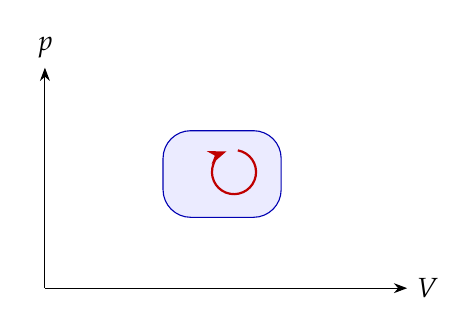
\begin{tikzpicture}[>=Stealth]
  \draw[->] (0,0)--(4.6,0) node[right] {$V$};
  \draw[->] (0,0)--(0,2.8) node[above] {$p$};
  \draw[blue!70!black,fill=blue!8,rounded corners=10pt] (1.5,0.9) rectangle (3.0,2.0);
  \draw[->,red!75!black,thick] (2.45,1.75) arc (80:-250:0.28);
\end{tikzpicture}
\caption{A thermodynamic cycle in the $(V,p)$ plane. Stokes' theorem identifies $\oint p\,\dd V$ with the enclosed area; the (clockwise) cycle delivers net work to the surroundings. No metric is involved.}
\label{fig:cycle}
\end{figure}

By Stokes (Green) in the $(V,p)$ plane,
\begin{align*}
\oint p\,\dd V&=\iint\dd(p\,\dd V) &&\text{(Stokes)}\\
&=\iint\dd p\wedge\dd V &&(\dd(p\,\dd V)=\dd p\wedge\dd V\text{ since }\dd\dd V=0)\\
&=-\iint\dd V\wedge\dd p &&\text{(antisymmetry)}\\
&=-\text{Area} &&\text{if the loop is counter-clockwise in the $(V,p)$ plane,}
\end{align*}
because $\dd V\wedge\dd p$ is the standard (positive) area form there. So a \emph{clockwise} cycle gives $+$Area (as in Figure~\ref{fig:cycle}): this is the net work delivered by the cycle. Since $\oint\dd U=0$, the first law gives $\oint\delta Q=\oint p\,\dd V$: the heat absorbed over a cycle equals the work delivered. Both are nonzero exactly when the loop encloses a nonzero area (if $\delta Q$ were exact, both would vanish).
Carath\'eodory (1909) formulated the second law as a statement about the Pfaffian form $\delta Q$: $1/T$ is an integrating factor, $\delta Q/T=\dd S$.

\subsection{Electromagnetism: which fields are $1$-forms, $2$-forms, $3$-forms?}\label{sec:phys-em}

With $\R^3$ as space, the natural degrees are:
\begin{center}
\small
\renewcommand{\arraystretch}{1.3}
\begin{tabular}{@{}p{5.2cm}p{1.8cm}p{6.0cm}@{}}
\toprule
\textbf{Field} & \textbf{Degree} & \textbf{Measured by}\\
\midrule
$E$ (electric field) & $1$-form & $\oint_\gamma E$ (e.m.f.), work per unit charge\\
$H$ (magnetic field strength) & $1$-form & $\oint_\gamma H$ (magnetomotive force)\\
$B$ (magnetic flux density) & $2$-form & $\int_SB$ (magnetic flux)\\
$D$ (electric displacement) & $2$-form & $\int_SD$ (electric flux)\\
$\rho$ (charge density) & $3$-form & $\int_\Omega\rho$ (charge)\\
$j$ (current density) & $2$-form & $\int_Sj$ (current)\\
$A$ (potential) & $1$-form & $\oint_\gamma A$ (holonomy / phase)\\
\bottomrule
\end{tabular}
\end{center}
($D$, $H$, $\rho$, $j$ are in fact \emph{twisted} forms: they also need an outer orientation, see Hehl--Obukhov or Burke.) The integral laws are then metric-free, being pure applications of Stokes' theorem:
\begin{alignat*}{2}
\oint_{\partial S}E&=-\frac{\dd}{\dd t}\int_SB&&\iff\dd E+\partial_tB=0\quad\text{(Faraday),}\\
\int_{\partial\Omega}B&=0&&\iff\dd B=0\quad\text{(no monopoles),}\\
\int_{\partial\Omega}D&=\int_\Omega\rho&&\iff\dd D=\rho\quad\text{(Gauss),}\\
\oint_{\partial S}H&=\int_Sj+\frac{\dd}{\dd t}\int_SD&&\iff\dd H=j+\partial_tD\quad\text{(Amp\`ere--Maxwell).}
\end{alignat*}
\emph{From integral to differential form (Faraday as an example).} By Stokes, $\oint_{\partial S}E=\int_S\dd E$; for a surface $S$ fixed in time, $-\frac{\dd}{\dd t}\int_SB=-\int_S\partial_tB$. So the law says $\int_S(\dd E+\partial_tB)=0$ for every surface $S$; a $2$-form whose integral over every small surface patch vanishes is itself zero, hence $\dd E+\partial_tB=0$. The same argument gives the other three.

The metric enters only through the \emph{constitutive relations} of the medium (vacuum): $D=\varepsilon_0\hodge E$, $B=\mu_0\hodge H$. Hence Gauss' law is topological, and the factor $E\cdot n\,\dd A$ of the usual statement hides $\varepsilon_0\hodge E$. In spacetime, $F=E\wedge\dd t+B$ and $\dd F=0$ is metric-free, while $\dd\hodge F=J$ needs $\hodge$ (in dimension $4$ the star on $2$-forms depends only on the conformal class of the metric, so Maxwell's equations are conformally invariant). Charge conservation is $\dd J=0$, and by Stokes $\int_{\partial\Omega}J=0$.
(In geometric algebra the two spacetime equations are the single equation $\vd F=J$, Section~\ref{sec:synth2}.)

\subhead{The Lorentz force and the interior product}
The force on a charge $q$ with velocity $v$ is the covector
\begin{equation}\label{eq:lorentz}
F=q\bigl(E-\iota_vB\bigr),\qquad\text{i.e. }F(w)=q\bigl(E(w)-B(v,w)\bigr).
\end{equation}
\emph{Derivation in $\R^3$ (steps).} Let $B=\iota_{\mathbf B}\vol$, \ie $B(a,b)=\vol(\mathbf B,a,b)$. The magnetic part of the Lorentz force is $F_{\mathrm{mag}}(w)=q\,(v\times\mathbf B)\cdot w$.
\begin{enumerate}
\item The scalar triple product is the volume form: $(v\times\mathbf B)\cdot w=\vol(v,\mathbf B,w)$.
\item Swap the first two arguments (alternating): $\vol(v,\mathbf B,w)=-\vol(\mathbf B,v,w)=-B(v,w)$.
\item Hence $F_{\mathrm{mag}}(w)=-q\,B(v,w)=-q\,(\iota_vB)(w)$, which proves the formula.
\end{enumerate}
The power is $F(v)=qE(v)-qB(v,v)=qE(v)$, because $B$ is alternating ($B(v,v)=0$): the magnetic force does no work for the same reason that $\iota_v\iota_v=0$.

\begin{example}[Amp\`ere's law and potentials: the angle form again]\label{ex:ampere}
Outside a wire carrying current $I$, the field has magnitude $I/(2\pi r)$ and points along $\hat\theta$, so, as a covector, $H=\frac I{2\pi r}e^\theta=\frac I{2\pi r}r\,\dd\theta=\frac I{2\pi}\dd\theta$ (using $e^\theta=r\,\dd\theta$). This is closed but not exact: $\oint H=I\neq0$, and there is no single-valued scalar potential even though $\dd H=0$.
The Aharonov--Bohm effect is the same phenomenon in quantum mechanics: the phase $\frac q\hbar\oint A$ along a loop around a solenoid is non-zero although $B=\dd A=0$ at every point of the loop. In the physical setup Stokes holds: $\oint A=\int_SB=\Phi$, the flux through the solenoid, because every surface $S$ bounded by the loop must cross the solenoid, where $B\neq0$. In the idealised thin-solenoid model the solenoid is removed from space; then $A$ is closed but not exact on the remaining region, exactly like $\frac I{2\pi}\dd\theta$ above, and no surface inside that region is bounded by the loop.
\end{example}

\subsection{Fluids: circulation needs a metric}\label{sec:phys-fluids}

The velocity field $u$ is a vector (it generates the flow). Its circulation $\Gamma=\oint_\gamma u^\flat$ integrates the covector $u^\flat=g(u,\cdot)$, so it needs a metric. The vorticity is the $2$-form $\dd u^\flat$ (the ``curl vector'' $\operatorname{curl}u=(\hodge\dd u^\flat)^\sharp$ again needs $g$ and the orientation). For a barotropic ideal fluid with enthalpy $h$, Euler's equation reads
\begin{equation}\label{eq:euler}
\partial_tu^\flat+\iota_u\dd u^\flat=-\dd\bigl(h+\tfrac12|u|^2\bigr).
\end{equation}
\emph{Where this equation comes from (steps).} (1) Euler: $\partial_tu+(u\cdot\nabla)u=-\nabla h$. (2) Vector identity: $(u\cdot\nabla)u=\nabla(\frac12|u|^2)-u\times\omega$ with $\omega=\operatorname{curl}u$. (3) Lower the index: $(u\times\omega)^\flat=-\iota_u\dd u^\flat$ (same triple-product computation as for the Lorentz force, with $\dd u^\flat=\iota_\omega\vol$). Substituting gives the stated equation.

\emph{Kelvin's theorem (steps).} By Cartan's formula \eqref{eq:cartan}, $\Lie_uu^\flat=\iota_u\dd u^\flat+\dd(\iota_uu^\flat)=\iota_u\dd u^\flat+\dd(|u|^2)$. Adding $\dd(|u|^2)$ to both sides of Euler's equation:
\[
(\partial_t+\Lie_u)u^\flat=\dd\bigl(\tfrac12|u|^2-h\bigr),
\]
an exact form. For a loop $\gamma(t)$ carried by the flow, $\frac{\dd}{\dd t}\oint_{\gamma(t)}u^\flat=\oint_{\gamma(t)}(\partial_t+\Lie_u)u^\flat=\oint\dd(\cdots)=0$, because exact forms integrate to zero on closed loops (Section~\ref{sec:expl-closed}). Kelvin's circulation theorem is Stokes plus this observation (Arnold--Khesin).

\subsection{Pseudovectors, torque and the cross product}\label{sec:phys-cross}

The cross product is $v\times w=\bigl(\hodge(v^\flat\wedge w^\flat)\bigr)^\sharp$: it needs a metric and an orientation, and it only produces a vector in dimension $3$ (in $\R^n$ the star turns the $2$-form $v^\flat\wedge w^\flat$ into an $(n-2)$-form).
\numcheck $v^\flat\wedge w^\flat=(v_xw_y-v_yw_x)\dd x\wedge\dd y+\cdots$ and $\hodge(\dd x\wedge\dd y)=\dd z$, so the $z$-component of the result is $v_xw_y-v_yw_x$, the familiar $(v\times w)_z$.
Angular momentum $L=x\wedge p$, torque $\tau=x\wedge F$ and the magnetic flux density $B$ are naturally $2$-forms (or bivectors); the ``axial vector'' $\mathbf B$ is $\hodge B$, which is why it does not flip sign under a reflection while a polar vector does. In relativity ($n=4$) there is no angular-momentum vector at all: $L^{\mu\nu}=x^\mu p^\nu-x^\nu p^\mu$ is an antisymmetric tensor.
In geometric algebra the same statement is $a\times b=(a\wedge b)\pss^{-1}$ (Section~\ref{sec:duality}): the bivector $a\wedge b$ is the physical object, and the cross product is its dual in $n=3$.

\subsection{Other classical sources of confusion}\label{sec:phys-confusion}

\begin{itemize}
\item \emph{``Is $\dd\mathbf r$ a vector or a covector?''} In $\int F_i\,\dd x^i$ the symbols $\dd x^i$ are covectors (differentials of coordinate functions), and the integral evaluates them on the displacement vector $\dot\gamma\,\dd t$. In $\int\mathbf F\cdot\dd\mathbf r$, $\dd\mathbf r$ denotes that displacement vector. Both notations compute the same contraction.
\item \emph{``Is the gradient a vector?''} $\dd V$ (components $\partial_iV$) is a covector; $\nabla V=g^{-1}\dd V$ is a vector and depends on the metric (Example~\ref{ex:twometrics}). They coincide numerically only in Cartesian coordinates with the Euclidean metric.
\item \emph{``Is the density $\rho$ a scalar?''} No: mass or charge density is an $n$-form (or a density) because it is integrated over volumes; under $x\mapsto\lambda x$ in $n$ dimensions it scales as $\lambda^{-n}$. It becomes a scalar function only after choosing a volume form $\mu$: $\rho=f\mu$.
\item \emph{``What needs what?''} $\dd$: nothing. grad: a metric. div: a volume form (a metric gives one). curl: a metric, an orientation and $n=3$. Laplacian $=\operatorname{div}\operatorname{grad}$: both.
\item \emph{``Does energy depend on the metric?''} The work integral does not; the kinetic energy does, through the inertia metric $g$, which is physical; and the relativistic energy depends on the observer $u$ through the pairing $-p(u)$.
\end{itemize}

\subsection{Dictionary: physical quantity $\to$ geometric object}\label{sec:phys-dict}

\begin{center}
\small
\renewcommand{\arraystretch}{1.3}
\begin{tabular}{@{}p{4.6cm}p{4.8cm}p{4.7cm}@{}}
\toprule
\textbf{Quantity} & \textbf{Geometric object} & \textbf{Is a metric needed?}\\
\midrule
Velocity $v$ & vector & no\\
Force $F$, momentum $p$ & $1$-forms (covectors) & no (but $p=g(v,\cdot)$ uses $g$)\\
Work $\int F$, power $F(v)$ & integral of a $1$-form, contraction & no\\
Kinetic energy $\frac12g(v,v)$ & quadratic form on velocities & yes: the inertia metric\\
Potential $V$; force $-\dd V$ & function; exact $1$-form & no ($\nabla V$ would need it)\\
Energy of a particle (relativity) $-p(u)$ & pairing with observer & $g$ only to build $p$\\
Conserved charges (Noether) $p(\xi)$, $\xi$ a symmetry & contraction & no\\
Action $\int(p\,\dd q-H\,\dd t)$ & integral of a $1$-form & no\\
Heat, thermodynamic work & non-closed $1$-forms & no metric exists\\
$E,H,A$ / $B,D,j$ / $\rho$ & $1$-forms / $2$-forms / $3$-form & no (only in $D=\varepsilon_0\hodge E,\dots$)\\
Circulation, vorticity $\oint u^\flat$, $\dd u^\flat$ & forms built from $u^\flat$ & yes, to form $u^\flat$\\
Cross product, $\mathbf B$, $L$, $\tau$ & $\hodge(a^\flat\wedge b^\flat)$, $2$-forms & metric $+$ orientation, $n=3$\\
\bottomrule
\end{tabular}
\end{center}

% =====================================================================
\section{Bridge to general relativity}\label{sec:bridge}
% =====================================================================

All the structures of Parts~\ref{part:algebra}--\ref{part:geometry} are what general relativity is made of. The following table (from source B) dictionary-translates physical statements; below it we add the
\emph{special-relativistic} content already met in Section~\ref{sec:phys-energy}.
% ---- begin extract GR lines 999-1028 ----

\begin{center}
\begin{tabular}{@{}p{4.1cm}p{5.1cm}p{5.2cm}@{}}
\toprule
\textbf{Mathematics} & \textbf{Physics} & \textbf{Where in this text}\\ \midrule
4-manifold $M$ & set of all events (spacetime) & Sec.~\ref{sec:manifolds}\\
Lorentzian metric $g_{\mu\nu}$, $\sig=(3,1)$ & gravitational field; proper time $\dd\tau^2=-g_{\mu\nu}\dd x^\mu\dd x^\nu$; light cones & Sec.~\ref{sec:metric},~\ref{sec:fields}\\
Timelike / null geodesic of $\nabla^{LC}$ & free fall of a massive particle / light ray & Sec.~\ref{sec:lc}\\
Killing vector field $\xi$ & symmetry $\Rightarrow$ conserved energy, momentum, angular momentum & Sec.~\ref{sec:lie},~\ref{sec:lc}\\
Christoffel symbols $\Gamma^\mu{}_{\nu\rho}$ & ``gravitational force'' seen by coordinates (can be removed locally) & Sec.~\ref{sec:conn}\\
Normal coordinates & local inertial frame (equivalence principle) & Sec.~\ref{sec:curv}\\
Riemann tensor $R^\mu{}_{\nu\rho\sigma}$ & tidal forces; $\ddot\xi=R(\dot\gamma,\xi)\dot\gamma$ & Sec.~\ref{sec:deviation}\\
Ricci tensor, scalar curvature & curvature produced by matter (Einstein equations) & Sec.~\ref{sec:curv}\\ \bottomrule
\end{tabular}
\end{center}

\begin{formal}[{Einstein's equations (preview)}]
Define the \emph{Einstein tensor} $G_{\mu\nu}=\Ric_{\mu\nu}-\tfrac12\,s\,g_{\mu\nu}$. The \emph{contracted second Bianchi identity} says $\nabla^\mu G_{\mu\nu}=0$ identically. Einstein's field equations (units $c=1$) are
\[
G_{\mu\nu}+\Lambda g_{\mu\nu}=8\pi G\,T_{\mu\nu},
\]
where $T_{\mu\nu}$ is the symmetric stress-energy tensor of matter, which satisfies $\nabla^\mu T_{\mu\nu}=0$ (local energy-momentum conservation); the identity above guarantees compatibility. In vacuum with $\Lambda=0$: taking the trace in 4 dimensions gives $s-2s=0\Rightarrow s=0$, hence $\Ric_{\mu\nu}=0$. The Schwarzschild metric
\[
\begin{aligned}\dd s^2={}&-\Big(1-\tfrac{2GM}{r}\Big)\dd t^2+\Big(1-\tfrac{2GM}{r}\Big)^{-1}\dd r^2\\&+r^2(\dd\theta^2+\sin^2\theta\,\dd\phi^2)\end{aligned}
\]
is such a Ricci-flat (but \emph{not} Riemann-flat) solution.
\end{formal}
\begin{intuition}[{the whole theory in one slogan}]
\emph{Matter tells spacetime how to curve (Einstein equations: $G\sim T$); spacetime tells matter how to move (geodesic equation).} Everything you have just learned is the vocabulary needed to write and understand this sentence. The remaining chapters of the course (special relativity review, principles of GR, Einstein equations and their consequences) use exactly these objects.
\end{intuition}
%% ---- end extract ----


\begin{synthesis}[energy, momentum and Killing fields on one page]
In the table above, the Killing-field row (``symmetry $\Rightarrow$ conserved energy, momentum, angular momentum'') for $\xi=\partial_t$ gives $E=-p(\xi)$, which is exactly the statement of Section~\ref{sec:phys-energy} that the energy of a particle measured by an observer $u$ is $-p(u)$: the Killing field is the observer who measures the conserved energy.
The signature convention is the mostly-plus one of Section~\ref{sec:metric}. The equation $G_{\mu\nu}=8\pi T_{\mu\nu}$ is, like the equation $\dd\hodge F=J$ of electromagnetism, an equation in which a metric-dependent operator ($\hodge$, resp.\ the Einstein tensor built from $R$) is equated to a source built from matter fields.
\end{synthesis}


\clearpage
% =====================================================================
\part{Complex analysis: the residue theorem as Stokes' theorem}\label{part:complex}
% =====================================================================

% =====================================================================
\section{The residue theorem as Stokes' theorem}\label{sec:complex}
% =====================================================================

Is the residue theorem related to all of this? Yes: it is not a separate theorem but Stokes' theorem applied to a particular kind of complex-valued $1$-form on a region with holes.
Cauchy's theorem is Stokes for a closed form; the residue theorem is Stokes for a closed form that fails to be exact exactly at the punctures, which is the mechanism of Example~\ref{ex:angle}
(the angle form $\dd\theta$ on $\R^2\setminus\{0\}$). Its real and imaginary parts are, respectively, the circulation and the flux of Sections~\ref{sec:stokes}--\ref{sec:phys}.

\subsection{Complex-valued $1$-forms and the contraction}\label{sec:complexforms}

Identify $\C=\R^2$ with $z=x+iy$. The form $\dd z=\dd x+i\,\dd y$ is a complex-valued $1$-form (a $\C$-valued covector at each point), and its contraction with a tangent vector $v=(v^x,v^y)\simeq v^x+iv^y$ is simply $\dd z(v)=v$. For a function $f:U\subset\C\to\C$ the form $f\,\dd z$ contracts with a velocity as $\langle f\,\dd z,\dot\gamma(t)\rangle=f(\gamma(t))\dot\gamma(t)$,
\begin{equation}\label{eq:cint}
\int_\gamma f\,\dd z=\int_a^bf(\gamma(t))\,\dot\gamma(t)\,\dd t,
\end{equation}
which is Definition~\eqref{eq:lineint} extended $\C$-linearly. For every smooth $f$ one has $\dd f=\partial_zf\,\dd z+\partial_{\bar z}f\,\dd\bar z$, and
\begin{equation}\label{eq:holo}
f\text{ holomorphic}\iff\partial_{\bar z}f=0\iff\dd f=f'(z)\,\dd z\iff\dd f_p:\R^2\to\C\text{ is }\C\text{-linear}.
\end{equation}
The Cauchy--Riemann equations are thus the statement that the covector $\dd f$ is complex-linear: $\dd f(iv)=i\,\dd f(v)$.

\emph{Steps behind these statements.} With $\partial_z=\frac12(\partial_x-i\partial_y)$ and $\partial_{\bar z}=\frac12(\partial_x+i\partial_y)$:
\begin{align*}
\partial_zf\,\dd z+\partial_{\bar z}f\,\dd\bar z&=\tfrac12(f_x-if_y)(\dd x+i\,\dd y)+\tfrac12(f_x+if_y)(\dd x-i\,\dd y)\\
&=\tfrac12\bigl(f_x\dd x+if_x\dd y-if_y\dd x+f_y\dd y\bigr)+\tfrac12\bigl(f_x\dd x-if_x\dd y+if_y\dd x+f_y\dd y\bigr)\\
&=f_x\dd x+f_y\dd y=\dd f.
\end{align*}
Writing $f=u+iv$, the condition $\partial_{\bar z}f=0$ means $f_x+if_y=(u_x-v_y)+i(v_x+u_y)=0$, \ie the usual Cauchy--Riemann equations $u_x=v_y$, $u_y=-v_x$. Finally $\dd f=f'\dd z$ means $\partial_{\bar z}f=0$ and $\partial_zf=f'$.

\subsection{Cauchy's theorem and the Cauchy--Riemann equations as ``$\operatorname{div}=0$, $\operatorname{curl}=0$''}\label{sec:cauchy}

Let us compute $\dd(f\,\dd z)$ in three steps.
\begin{enumerate}
\item Leibniz rule and $\dd(\dd z)=0$: $\dd(f\,\dd z)=\dd f\wedge\dd z$.
\item Insert $\dd f=\partial_zf\,\dd z+\partial_{\bar z}f\,\dd\bar z$ and use $\dd z\wedge\dd z=0$: $\dd f\wedge\dd z=\partial_{\bar z}f\,\dd\bar z\wedge\dd z$.
\item Expand $\dd\bar z\wedge\dd z=(\dd x-i\,\dd y)\wedge(\dd x+i\,\dd y)=i\,\dd x\wedge\dd y-i\,\dd y\wedge\dd x=2i\,\dd x\wedge\dd y$.
\end{enumerate}
\begin{equation}\label{eq:dfdz}
\dd(f\,\dd z)=\partial_{\bar z}f\,\dd\bar z\wedge\dd z=2i\,\partial_{\bar z}f\,\dd x\wedge\dd y .
\end{equation}
Hence $f$ is holomorphic if and only if the $1$-form $f\,\dd z$ is closed, and Stokes' theorem gives at once

\begin{theorem}[Cauchy]\label{thm:cauchy}
If $f$ is holomorphic on a neighbourhood of a compact region $\Omega\subset\C$ with piecewise smooth boundary, then
$\displaystyle\oint_{\partial\Omega}f\,\dd z=\int_\Omega\dd(f\,\dd z)=0.$
\end{theorem}

\subhead{Real and imaginary parts: circulation and flux}
Write $w=u-iv$ (the ``complex velocity'' of a planar vector field $\mathbf u=(u,v)$). Then
\begin{equation}\label{eq:wdz}
w\,\dd z=\underbrace{(u\,\dd x+v\,\dd y)}_{\mathbf u^\flat}+i\underbrace{(u\,\dd y-v\,\dd x)}_{\iota_{\mathbf u}(\dd x\wedge\dd y)=\hodge\mathbf u^\flat}.
\end{equation}
The real part is the covector $\mathbf u^\flat$ (its integral is the circulation $\Gamma$), and the imaginary part is the contraction $\iota_{\mathbf u}\vol$ (its integral is the flux $Q$ through the curve, cf.\ \eqref{eq:flux}). The split follows from $w\,\dd z=(u-iv)(\dd x+i\,\dd y)=u\,\dd x+iu\,\dd y-iv\,\dd x+v\,\dd y$ and from $\iota_{\mathbf u}(\dd x\wedge\dd y)=u\,\dd y-v\,\dd x$ (Example~\ref{ex:interiorplane}). Moreover, from \eqref{eq:dfdz}, in steps:
\[
\partial_{\bar z}w=\tfrac12(\partial_x+i\partial_y)(u-iv)=\tfrac12\bigl[(u_x+v_y)+i(u_y-v_x)\bigr]=\tfrac12\bigl(\operatorname{div}\mathbf u-i\operatorname{curl}\mathbf u\bigr)
\]
(with $\operatorname{curl}\mathbf u=\partial_xv-\partial_yu$), 
so \emph{$w$ is holomorphic $\iff$ the flow is incompressible ($\operatorname{div}\mathbf u=0$) and irrotational ($\operatorname{curl}\mathbf u=0$).}
Cauchy's theorem is then Green's theorem (Kelvin--Stokes in the plane) for the real part and the divergence theorem (Gauss) for the imaginary part, both applied at the same time.

\begin{specialcase}[the Hodge star in dimension two]\label{sc:hodge2}
In the language of Section~\ref{sec:classical}, in dimension two the Hodge star on $1$-forms satisfies $\hodge\dd z=-i\,\dd z$ and $\hodge\dd\bar z=i\,\dd\bar z$: $\dd z$ is an eigenform of $\hodge$, and since $\hodge$ on $1$-forms depends only on the conformal class of the metric, holomorphy is a conformally invariant notion (conformal maps preserve holomorphic functions). The eigenform property is checked in one line: $\hodge\dd x=\dd y$, $\hodge\dd y=-\dd x$, so $\hodge\dd z=\dd y-i\,\dd x=-i(\dd x+i\,\dd y)=-i\,\dd z$.
\end{specialcase}

\subsection{The residue theorem}\label{sec:residue}

Let $f$ be holomorphic on an open set containing $\overline\Omega$ except at finitely many points $a_1,\dots,a_k\in\Omega$ where it has isolated singularities (poles or essential singularities). The \emph{residue} of $f$ at $a$ is the coefficient $c_{-1}$ of its Laurent expansion $f(z)=\sum_nc_n(z-a)^n$, equivalently
\begin{equation}\label{eq:residue}
\Res_af=\frac1{2\pi i}\oint_{|z-a|=\varepsilon}f\,\dd z\qquad(\text{small }\varepsilon>0,\ \text{counter-clockwise}).
\end{equation}
\emph{Why the two definitions agree (steps).} Parametrise the circle: $z=a+\varepsilon e^{it}$, $t\in[0,2\pi]$, so $\dd z=i\varepsilon e^{it}\,\dd t$. For an integer $n$:
\[
\oint(z-a)^n\,\dd z=\int_0^{2\pi}\varepsilon^ne^{int}\,i\varepsilon e^{it}\,\dd t=i\varepsilon^{n+1}\int_0^{2\pi}e^{i(n+1)t}\,\dd t=\begin{cases}2\pi i,&n=-1,\\0,&n\neq-1,\end{cases}
\]
because for $m=n+1\neq0$, $\int_0^{2\pi}e^{imt}\,\dd t=\bigl[e^{imt}/(im)\bigr]_0^{2\pi}=0$, while for $m=0$ the integrand is $1$. Integrating the Laurent series term by term (it converges uniformly on the circle) leaves only $c_{-1}\cdot2\pi i$.

\begin{figure}[ht]
\centering
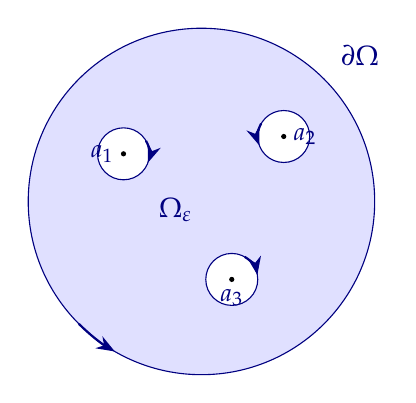
\begin{tikzpicture}[>=Stealth,scale=1.1]
  \fill[blue!12] (0,0) circle (2.0);
  \draw[navy] (0,0) circle (2.0);
  \foreach \c/\n in {(-0.9,0.55)/1,(0.95,0.75)/2,(0.35,-0.9)/3}{
     \fill[white] \c circle (0.3);
     \draw[navy] \c circle (0.3);
     \fill \c circle (0.03);
  }
  \node[navy,left] at (-0.9,0.55) {\small$a_1$};
  \node[navy,right] at (0.95,0.75) {\small$a_2$};
  \node[navy,below] at (0.35,-0.9) {\small$a_3$};
  \node[navy] at (-0.3,-0.1) {$\Omega_\varepsilon$};
  \node[navy,above right] at (1.5,1.45) {$\partial\Omega$};
  \draw[->,navy,thick] (225:2.0) arc (225:240:2.0);
  \draw[->,navy,thick] ($(-0.9,0.55)+(30:0.3)$) arc (30:-20:0.3);
  \draw[->,navy,thick] ($(0.95,0.75)+(150:0.3)$) arc (150:200:0.3);
  \draw[->,navy,thick] ($(0.35,-0.9)+(60:0.3)$) arc (60:10:0.3);
\end{tikzpicture}
\caption{Proof of the residue theorem. Stokes on $\Omega_\varepsilon=\Omega$ minus small discs: the outer boundary runs counter-clockwise and the small circles clockwise (region on the left). Since $f\,\dd z$ is closed on $\Omega_\varepsilon$, the integral over the outer boundary equals the sum of the integrals over the small circles traversed counter-clockwise. This is the annulus of Figure~\ref{fig:annulus} with several holes.}
\label{fig:residue}
\end{figure}

\begin{theorem}[Residue theorem]\label{thm:residue}
Under these assumptions,
\[
\oint_{\partial\Omega}f\,\dd z=2\pi i\sum_{j=1}^k\Res_{a_j}f .
\]
\end{theorem}
\begin{proof}
Remove from $\Omega$ small open discs $D_j=D(a_j,\varepsilon)$ and let $\Omega_\varepsilon=\Omega\setminus\bigcup_jD_j$, a manifold with boundary $\partial\Omega_\varepsilon=\partial\Omega-\sum_j\partial D_j$ (the circles are traversed clockwise: induced orientation, Figure~\ref{fig:residue}). On $\Omega_\varepsilon$ the form $f\,\dd z$ is smooth and closed, so Stokes' theorem \eqref{eq:stokes} gives
\[
0=\int_{\Omega_\varepsilon}\dd(f\,\dd z)=\oint_{\partial\Omega}f\,\dd z-\sum_j\oint_{\partial D_j^{\mathrm{ccw}}}f\,\dd z,
\]
and each small-circle integral is $2\pi i\Res_{a_j}f$ by \eqref{eq:residue}.
\end{proof}

\begin{example}[Two applications of the residue theorem]\label{ex:residues}
(a) $\displaystyle\oint_{|z|=2}\frac{\dd z}{z(z-1)}$. Partial fractions: $\frac1{z(z-1)}=\frac1{z-1}-\frac1z$, so $\Res_1=+1$ and $\Res_0=-1$ (both poles lie inside $|z|<2$). The theorem gives $2\pi i(1-1)=0$.
\emph{Check:} $\oint\frac{\dd z}{z-1}=2\pi i$ and $\oint\frac{\dd z}z=2\pi i$ by the circle computation above, and their difference is $0$.

(b) $\displaystyle\oint_{|z|=1}\frac{e^z}{z^2}\,\dd z$. Expand $e^z=1+z+\frac{z^2}2+\cdots$, so $\frac{e^z}{z^2}=\frac1{z^2}+\frac1z+\frac12+\cdots$ and $c_{-1}=1$. The integral is $2\pi i\cdot1=2\pi i$. (Equivalently, $\Res_0=\frac{\dd}{\dd z}e^z\big|_0=1$, the formula for a double pole.)
\end{example}

\begin{keyidea}[why only $c_{-1}$ survives: exact versus closed]
On $\C\setminus\{a\}$ the forms $(z-a)^n\dd z$ with $n\neq-1$ are \emph{exact}: $(z-a)^n\dd z=\dd\bigl(\frac{(z-a)^{n+1}}{n+1}\bigr)$, so they integrate to zero on any closed loop (Section~\ref{sec:expl-closed}). The only closed, non-exact one is
\begin{equation}\label{eq:dzoverz}
\frac{\dd z}{z-a}=\dd\ln|z-a|+i\,\dd\theta,
\end{equation}
whose imaginary part is precisely the angle form $\dd\theta$ of Example~\ref{ex:angle}, with $\oint\dd\theta=2\pi$; hence $\oint\frac{\dd z}{z-a}=i\cdot2\pi=2\pi i$. Derivation of the identity: write $z=re^{i\theta}$; then $\dd z=e^{i\theta}\dd r+ire^{i\theta}\dd\theta$ and $\frac{\dd z}z=\frac{\dd r}r+i\,\dd\theta=\dd\ln r+i\,\dd\theta$.
In other words, the residue measures the component of $f\,\dd z$ along the one cohomology class which is not exact near $a$.
\end{keyidea}

\subsection{The cohomological meaning of the residue}\label{sec:rescohom}

For $X=\C\setminus\{a_1,\dots,a_k\}$ one has $H^1_{\mathrm{dR}}(X;\C)\cong\C^k$, generated by the classes of $\dd z/(z-a_j)$, and $H_1(X;\Z)\cong\Z^k$, generated by small circles around the $a_j$. The residue is the de Rham pairing between these:
$\Res_{a_j}f=\frac1{2\pi i}\bigl\langle[\text{circle around }a_j],[f\,\dd z]\bigr\rangle$.
A closed loop $\gamma$ in $X$ is homologous to $\sum_jn_j[\text{circle}_j]$, where $n_j=\frac1{2\pi i}\oint_\gamma\frac{\dd z}{z-a_j}$ is the winding number of $\gamma$ around $a_j$ (Example~\ref{ex:angle}); \eg a loop that goes twice around $a_j$ has $\oint\frac{\dd z}{z-a_j}=2\cdot2\pi i$, so $n_j=2$. This yields the general version
\begin{equation}\label{eq:winding}
\oint_\gamma f\,\dd z=2\pi i\sum_jn(\gamma,a_j)\Res_{a_j}f .
\end{equation}
The integral depends only on the homology class of the contour: a contour can be deformed freely as long as it does not cross a singularity, which is the practical principle behind contour integration.

\subsection{Beyond holomorphic functions: Cauchy--Pompeiu and the Coulomb law in 2D}\label{sec:pompeiu}

If $f$ is merely smooth, Stokes still applies. Let us derive the Cauchy--Pompeiu formula step by step, with $\omega=\dfrac{f\,\dd z}{z-z_0}$ on $\Omega_\varepsilon=\Omega\setminus D(z_0,\varepsilon)$.
\begin{enumerate}
\item \emph{Differentiate.} $1/(z-z_0)$ is holomorphic away from $z_0$, so $\partial_{\bar z}\bigl(f/(z-z_0)\bigr)=\partial_{\bar z}f/(z-z_0)$ and, by \eqref{eq:dfdz}, $\dd\omega=\dfrac{\partial_{\bar z}f}{z-z_0}\,2i\,\dd x\wedge\dd y$.
\item \emph{Stokes on $\Omega_\varepsilon$} (outer boundary ccw, small circle cw): $\displaystyle\oint_{\partial\Omega}\omega-\oint_{|z-z_0|=\varepsilon}\omega=\int_{\Omega_\varepsilon}\dd\omega$.
\item \emph{The small circle.} With $z=z_0+\varepsilon e^{it}$: $\displaystyle\oint\omega=\int_0^{2\pi}\frac{f(z_0+\varepsilon e^{it})}{\varepsilon e^{it}}\,i\varepsilon e^{it}\,\dd t=i\int_0^{2\pi}f(z_0+\varepsilon e^{it})\,\dd t\xrightarrow[\varepsilon\to0]{}2\pi if(z_0)$ by continuity of $f$.
\item \emph{Let $\varepsilon\to0$.} The area integral converges because $1/|z-z_0|$ is integrable in the plane (area element $r\,\dd r\,\dd\theta$). We get $\displaystyle\oint_{\partial\Omega}\frac{f\,\dd z}{z-z_0}-2\pi if(z_0)=2i\iint_\Omega\frac{\partial_{\bar z}f}{z-z_0}\,\dd A$.
\item \emph{Divide by $2\pi i$ and solve for $f(z_0)$:}
\begin{equation}\label{eq:pompeiu}
f(z_0)=\frac1{2\pi i}\oint_{\partial\Omega}\frac{f(z)}{z-z_0}\,\dd z-\frac1\pi\iint_\Omega\frac{\partial_{\bar z}f}{z-z_0}\,\dd A .
\end{equation}
\end{enumerate}
For holomorphic $f$ the area term vanishes and we recover Cauchy's integral formula. In the language of distributions the same computation says $\partial_{\bar z}\bigl(\frac1{\pi z}\bigr)=\delta_0$, \ie $1/(\pi z)$ is the fundamental solution of $\partial_{\bar z}$, in perfect analogy with the Gauss law in the plane (Section~\ref{sec:phys-em}): a point charge $Q$ (or a point vortex with circulation $\Gamma$ and source $Q$) is a simple pole of the complex field $w$ whose residue encodes the charge: $\Res_0w=\frac{\Gamma+iQ}{2\pi i}$, \ie $2\pi i\Res_0w=\Gamma+iQ$,
\[
w(z)=\frac{\Gamma+iQ}{2\pi i}\,\frac1z\quad\Longrightarrow\quad\oint w\,\dd z=\Gamma+iQ .
\]
This is why the residue theorem reads, in electrostatics or fluid mechanics, as ``the total flux (and circulation) through a curve equals the sum of the charges (vortices) inside''.

\subsection{The argument principle: counting zeros with a $1$-form}\label{sec:argument}

Let $f$ be meromorphic on a neighbourhood of the closure of $\Omega$, with no zeros or poles on $\partial\Omega$. Then $\frac{f'}f\dd z=\dd\log f=\dd\ln|f|+i\,\dd\arg f=f\pb\bigl(\frac{\dd z}z\bigr)$. The first term is exact, so the residue theorem becomes
\begin{equation}\label{eq:argument}
\frac1{2\pi i}\oint_{\partial\Omega}\frac{f'}f\,\dd z=\frac1{2\pi}\oint_{\partial\Omega}f\pb\dd\theta=N-P,
\end{equation}
where $N$ and $P$ are the numbers of zeros and poles in $\Omega$ counted with multiplicity: the winding number of the curve $f(\partial\Omega)$ around $0$.
\emph{Steps.} (1) Locally $\log f=\ln|f|+i\arg f$, and $\dd\log f=\frac{\dd f}f=\frac{f'}f\dd z$; this is also the pull-back $f\pb(\dd z/z)$ because $f\pb\dd z=\dd f=f'\dd z$. (2) $\dd\ln|f|$ is exact, so its integral over a closed curve is $0$. (3) What remains is $i\oint\dd\arg f=2\pi i\cdot(\text{winding number of }f\circ\gamma\text{ around }0)$.
(4) By the residue theorem, $\frac{f'}f$ has a simple pole with residue $+m$ at a zero of order $m$ and $-m$ at a pole of order $m$ (since $f=(z-a)^{\pm m}g$ gives $f'/f=\pm m/(z-a)+g'/g$).
\numcheck $f(z)=z^2$ on $|z|=1$: $\frac{f'}f=\frac2z$, $\frac1{2\pi i}\oint\frac2z\,\dd z=2=N$ (a double zero at the origin), and $f(e^{it})=e^{2it}$ winds twice around $0$.
This is the degree of the map $f|_{\partial\Omega}:\partial\Omega\to\C\setminus\{0\}$, computed by pulling back the angle form (Section~\ref{sec:stokes}), and it is the basis of Rouch\'e's theorem and of the fundamental theorem of algebra.

\begin{example}[A real integral by residues, step by step]\label{ex:realint}
To compute $I=\displaystyle\int_{-\infty}^\infty\frac{\dd x}{1+x^2}$, apply Theorem~\ref{thm:residue} to $f\,\dd z$ with $f=\dfrac1{1+z^2}$ on the upper half-disc $\Omega_R$ of radius $R>1$, whose boundary is the segment $[-R,R]$ followed by the semicircle $C_R$.
\begin{enumerate}
\item \emph{Poles.} $1+z^2=(z-i)(z+i)$; only $z=i$ lies inside $\Omega_R$.
\item \emph{Residue.} $\Res_if=\lim_{z\to i}\frac{z-i}{(z-i)(z+i)}=\frac1{2i}$.
\item \emph{Theorem.} $\int_{-R}^Rf(x)\,\dd x+\int_{C_R}f\,\dd z=2\pi i\cdot\frac1{2i}=\pi$. (On the real axis the pull-back of $f\,\dd z$ is $f(x)\,\dd x$, the contraction with the velocity $1$.)
\item \emph{The arc vanishes.} On $|z|=R$, $|1+z^2|\ge R^2-1$, so $\bigl|\int_{C_R}f\,\dd z\bigr|\le\dfrac{\pi R}{R^2-1}\to0$ as $R\to\infty$ (length $\pi R$ times the bound on $|f|$).
\item \emph{Limit.} Letting $R\to\infty$: $I=\pi$.
\end{enumerate}
\emph{Check:} $\int\frac{\dd x}{1+x^2}=\arctan x\big|_{-\infty}^\infty=\frac\pi2-(-\frac\pi2)=\pi$ \checkmark.
\end{example}

\subsection{The current picture}\label{sec:rescurrent}

\begin{itemize}
\item \emph{Riemann surfaces.} If $\eta$ is a meromorphic $1$-form on a compact Riemann surface $S$ (no boundary), Stokes with small discs removed gives $\sum_{p\in S}\Res_p\eta=0$: the sum of all residues vanishes. Combined with Poincar\'e/Serre duality this is a key ingredient in the proofs of the Riemann--Roch theorem and in the theory of abelian differentials. Note that this statement does not even need a metric: $\eta$ is a $1$-form and $\Res_p\eta$ is intrinsic, which is why residues are defined for forms $f\,\dd z$ and not for functions $f$ (the residue of the function $f$ changes under a change of coordinate $z\mapsto h(z)$, that of the form $f\,\dd z$ does not).
\item \emph{Several complex variables.} The kernel $1/(z-z_0)$ is replaced by the Bochner--Martinelli kernel, and residues by Poincar\'e--Leray residues of closed forms with poles along hypersurfaces; both are proved with Stokes' theorem and are expressed through de Rham cohomology of the complement of the singular set.
\item \emph{Currents.} Formulae such as $\partial_{\bar z}(1/\pi z)=\delta_0$ and the Poincar\'e--Lelong formula $\frac i\pi\partial\bar\partial\log|f|=[\{f=0\}]$ treat the residue as the current of integration over the singular set (Section~\ref{sec:current}, item~3), exactly as Stokes' theorem is treated in geometric measure theory.
\end{itemize}

\begin{center}
\small
\renewcommand{\arraystretch}{1.3}
\begin{tabular}{@{}p{4.6cm}p{9.6cm}@{}}
\toprule
\textbf{Complex analysis} & \textbf{Differential forms}\\
\midrule
$f$ holomorphic & $f\,\dd z$ closed; $\dd f$ is $\C$-linear\\
Cauchy's theorem & Stokes for a closed form on $\Omega$\\
Cauchy--Riemann equations & $\operatorname{div}=0$ and $\operatorname{curl}=0$ (real/imaginary parts of $w\,\dd z$)\\
Residue $\Res_af$ & period of $f\,\dd z$ over a small circle $=$ de Rham pairing\\
Residue theorem & Stokes on $\Omega$ minus discs; boundary $=$ outer curve $-$ small circles\\
Winding number, argument principle & $\frac1{2\pi}\oint f\pb\dd\theta=$ degree of a map to $S^1$\\
Cauchy--Pompeiu, $\partial_{\bar z}(1/\pi z)=\delta$ & Stokes with $\dd\omega\neq0$; Gauss law in the plane\\
\bottomrule
\end{tabular}
\end{center}

\subsection{Synthesis IV: complex analysis in the geometric algebra of the plane}\label{sec:synth4}

\begin{synthesis}[where does the imaginary unit come from?]
The symbol $i$ has appeared in three guises. (1) As a scalar: $\C=\Cl(0,1)$, the geometric algebra of a line with $e^2=-1$ (Section~\ref{sec:clifford}). (2) As a bivector: in the plane algebra $\Cl(2,0)$ the unit area element $\pss=e_1e_2$ satisfies $\pss^2=-1$, and the even subalgebra $\{x+\pss y\}$ is $\C$; multiplying a vector on the left by $e_1$ identifies $\R^2$ with $\C$, $e_1(x+\pss y)=xe_1+ye_2$. (3) As the factor in complex-valued forms such as $\dd z=\dd x+i\,\dd y$, where $i$ is a formal scalar commuting with everything.
In option (2) $i$ is the \emph{oriented plane itself}, and ``multiplication by $i$'' is a quarter-turn \emph{because} $\pss$ rotates vectors by $90^\circ$ under the geometric product: the dual of a vector in $2$D is the vector turned by a quarter turn (Section~\ref{sec:duality}).
\end{synthesis}

\begin{proposition}[Cauchy--Riemann as a single multivector equation]\label{prop:CRga}
Let $\mathbf u=u\,e_1+v\,e_2$ be a vector field in the plane, $\vd=e_1\partial_x+e_2\partial_y$, $\pss=e_1e_2$, and $w=u-iv$ the complex velocity of \eqref{eq:wdz}. Then
\[
\vd\,\mathbf u=\operatorname{div}\mathbf u+\pss\,\operatorname{curl}\mathbf u=2\,\partial_z\bar w,
\]
so $w$ is holomorphic if and only if $\vd\mathbf u=0$ (a \emph{monogenic} function).
\end{proposition}
\begin{proof}
$\vd\mathbf u=(e_1\partial_x+e_2\partial_y)(ue_1+ve_2)=(u_x+v_y)+e_1e_2(v_x-u_y)$, using $e_1e_2=-e_2e_1$ and $e_i^2=1$; this is $\operatorname{div}\mathbf u+\pss\operatorname{curl}\mathbf u$. On the other hand $2\partial_z\bar w=(\partial_x-i\partial_y)(u+iv)=(u_x+v_y)+i(v_x-u_y)$ with $i\leftrightarrow\pss$. Holomorphy of $w$ means $\partial_{\bar z}w=0$, whose conjugate is $\partial_z\bar w=0$.
\end{proof}

\begin{example}[a monogenic field]\label{ex:monogenic}
$w=z^2=(x^2-y^2)+2ixy$. Since $w=u-iv$, we read off $u=x^2-y^2$ and $v=-2xy$. Then $\operatorname{div}\mathbf u=2x-2x=0$ and $\operatorname{curl}\mathbf u=v_x-u_y=-2y+2y=0$, so $\vd\mathbf u=0$ \checkmark.
\end{example}

\begin{synthesis}[Cauchy's theorem, three ways]
\emph{Forms:} $\dd(f\,\dd z)=2i\,\partial_{\bar z}f\,\dd x\wedge\dd y$ (equation \eqref{eq:dfdz}) and Stokes. \emph{Vector calculus:} Green's theorem for the real part and the divergence theorem for the imaginary part of \eqref{eq:wdz}. \emph{Geometric algebra:} the single equation $\vd\mathbf u=0$ of Proposition~\ref{prop:CRga}; in higher dimension the same equation $\vd F=0$ defines monogenic functions (Clifford analysis), for which an analogue of Cauchy's integral formula holds (Hestenes--Sobczyk, Section~\ref{sec:refs}).
\end{synthesis}


\clearpage
% =====================================================================
\part{Perspective: current state and master summary}\label{part:perspective}
% =====================================================================

% =====================================================================
\section{The current state of the subject}\label{sec:current}
% =====================================================================

The statements above are the standard, textbook (``smooth'') form of the theorems (Spivak, Lee, Bott--Tu). Active and established developments extend them in several directions.

\begin{enumerate}
\item \textbf{Conceptual unification.} Since the early twentieth century (Poincar\'e, Cartan, de Rham) the gradient theorem, Green, Kelvin--Stokes and Gauss are viewed as one theorem, \eqref{eq:stokes}, equivalent to the duality \eqref{eq:adjoint}. The 19th-century formulations (Gauss, Green, Ostrogradsky, Kelvin, Stokes) are recovered by the dictionary $\flat,\sharp,\hodge$ (Section~\ref{sec:classical}); the geometric-algebra formulation of the same dictionary is Section~\ref{sec:synth2}.
\item \textbf{Rough domains and non-smooth data.} Stokes holds for manifolds with corners and piecewise smooth chains, and for Lipschitz domains (with the normal defined almost everywhere and traces of Sobolev fields). The De Giorgi--Federer divergence theorem holds for sets $E$ of finite perimeter:
\[
\int_E\operatorname{div}X\,\dd x=\int_{\partial^*E}X\cdot\nu_E\,\dd\mathcal H^{n-1},
\]
where $\partial^*E$ is the reduced boundary and $\nu_E$ the measure-theoretic outer normal; no topological regularity of $\partial E$ is required.
\item \textbf{Geometric measure theory: Stokes as a definition.} In the theory of currents (de Rham, Federer--Fleming) a $k$-current is a continuous linear functional $T$ on compactly supported $k$-forms, and the boundary is defined by $(\partial T)(\alpha)=T(\dd\alpha)$, \ie Stokes' formula \eqref{eq:adjoint} becomes an axiom. Whitney's flat chains and Harrison's chainlets give Stokes' theorem for very irregular (even fractal) domains.
\item \textbf{Discrete and numerical versions.} On a simplicial or cell complex, Stokes' theorem holds exactly: the coboundary operator is the transpose of the boundary matrix. This is the foundation of discrete exterior calculus and finite element exterior calculus (Arnold--Falk--Winther), and of structure-preserving discretisations of Maxwell's equations and fluid dynamics that conserve fluxes to machine precision.
\item \textbf{Cohomological and topological consequences.} Stokes' theorem underlies de Rham's theorem, Poincar\'e duality ($\int_M\alpha\wedge\beta$ pairs $H^k$ with $H^{n-k}$ on compact oriented $M$), degree theory and characteristic classes (via Chern--Weil theory), and the integral laws of electromagnetism and conservation laws in continuum mechanics and general relativity.
\item \textbf{Geometric algebra and Clifford analysis.} The vector derivative $\vd$ and its monogenic functions (Section~\ref{sec:synth4}) generalise holomorphic function theory to every dimension; the Clifford algebras of Section~\ref{sec:clifford} underlie spin geometry and the Dirac operator, and the geometric-calculus form of Stokes' theorem is the subject of Hestenes--Sobczyk.
\end{enumerate}

% =====================================================================
\section{Master summary}\label{sec:summary}
% =====================================================================

\subsection{One picture}

\begin{figure}[ht]
\centering
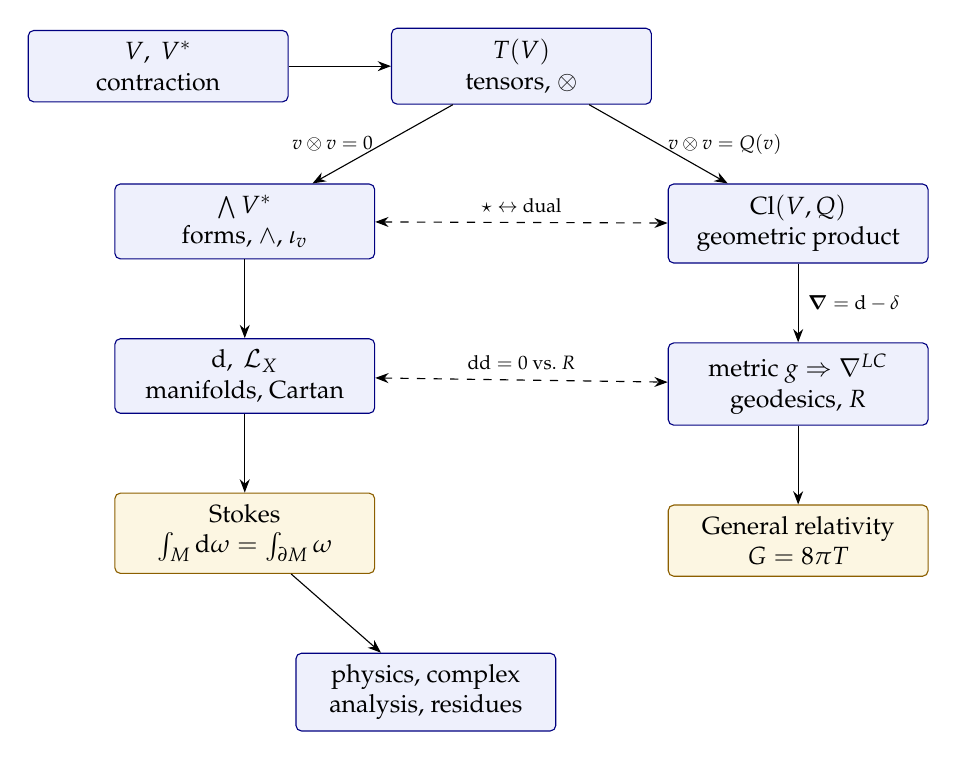
\begin{tikzpicture}[>=Stealth,node distance=0.9cm and 1.3cm,
   box/.style={draw=navy,fill=kiback,rounded corners=2pt,align=center,inner sep=4pt,font=\small,minimum width=3.3cm},
   syn/.style={draw=synthfr,fill=synthbg,rounded corners=2pt,align=center,inner sep=4pt,font=\small,minimum width=3.3cm}]
  \node[box] (vv) {$V,\ V^*$\\ contraction};
  \node[box,right=of vv] (tt) {$T(V)$\\ tensors, $\otimes$};
  \node[box,below left=1.0cm and 0.2cm of tt] (ext) {$\bigwedge V^*$\\ forms, $\wedge$, $\iota_v$};
  \node[box,below right=1.0cm and 0.2cm of tt] (cl) {$\Cl(V,Q)$\\ geometric product};
  \node[box,below=1.0cm of ext] (dd) {$\dd,\ \Lie_X$\\ manifolds, Cartan};
  \node[box,below=1.0cm of cl] (met) {metric $g\Rightarrow\nabla^{LC}$\\ geodesics, $R$};
  \node[syn,below=1.0cm of dd] (stk) {Stokes\\ $\int_M\dd\omega=\int_{\partial M}\omega$};
  \node[syn,below=1.0cm of met] (gr) {General relativity\\ $G=8\pi T$};
  \node[box,below=1.0cm of stk,xshift=2.3cm] (phys) {physics, complex\\ analysis, residues};
  \draw[->] (vv)--(tt);
  \draw[->] (tt)--node[left,font=\scriptsize]{$v\otimes v=0$}(ext);
  \draw[->] (tt)--node[right,font=\scriptsize]{$v\otimes v=Q(v)$}(cl);
  \draw[->] (ext)--(dd);
  \draw[->] (cl)--node[right,font=\scriptsize]{$\vd=\dd-\codiff$}(met);
  \draw[<->,dashed] (ext)--node[above,font=\scriptsize]{$\hodge\leftrightarrow$ dual}(cl);
  \draw[->] (dd)--(stk);
  \draw[->] (met)--(gr);
  \draw[->] (stk)--(phys);
  \draw[<->,dashed] (dd)--node[above,font=\scriptsize]{$\dd\dd=0$ vs.\ $R$}(met);
\end{tikzpicture}
\caption{The logical structure of the document. Solid arrows: ``is used to build''; dashed: the comparisons made in the synthesis sections.}
\label{fig:map}
\end{figure}

\subsection{The essence of each concept}

{\small
\renewcommand{\arraystretch}{1.3}
\begin{longtable}{@{}p{3.6cm}p{10.4cm}@{}}
\toprule
\textbf{Concept} & \textbf{Essence}\\
\midrule
\endhead
Contraction $\omega(v)=\omega_iv^i$ & canonical pairing $V^*\times V\to\R$; needs no metric. First case $\iota_v\omega$ of the interior product.\\
Exterior product $\alpha\wedge\beta$ & antisymmetrised tensor product, a determinant on $1$-forms; graded commutative; $\dd x$ is the covector dual to $\partial/\partial x$, with $\dd x(\partial_x)=1$.\\
$\int_\gamma\omega$ & contract $\omega$ with the velocity, integrate in $t$: $\int\omega(\dot\gamma)\,\dd t=\int_\gamma\gamma\pb\omega$. Linearity $\Rightarrow$ reparametrisation invariance and sign change with orientation.\\
$\int_\phi\alpha$ & full contraction with the tangent $k$-frame, then Lebesgue integration.\\
Flux $\int_\Sigma\iota_X\mu$ & partial contraction of a volume form with a vector field; volume swept per unit time.\\
Stokes & $\int_M\dd\omega=\int_{\partial M}\omega\iff\dd$ and $\partial$ are adjoint.\\
Gauss & Stokes applied to $\omega=\iota_X\mu$, using $\dd\iota_X\mu=\Lie_X\mu=\operatorname{div}_\mu X\,\mu$.\\
Physics & work $\int F$ is intrinsic (force is a covector); the metric appears only as inertia (kinetic energy), as the vacuum (constitutive laws) or via an observer; fluxes are $2$-forms, charges $3$-forms.\\
Residues & $f\,\dd z$ is closed iff $f$ is holomorphic; $\oint f\,\dd z=2\pi i\sum\Res$ is Stokes on $\Omega$ minus discs. Real part $=$ circulation, imaginary part $=$ flux; the residue is the period over a small circle (de Rham pairing).\\
Geometric algebra & $uv=u\cdot v+u\wedge v$: one product containing the metric and the wedge; $\dd\leftrightarrow\vd\wedge$; one operator $\vd$ for grad, curl, div; $\vd F=J$.\\
Curvature & failure of covariant derivatives to commute: $[\nabla_X,\nabla_Y]-\nabla_{[X,Y]}=R(X,Y)$; the nonzero analogue of $\dd\dd=0$.\\
\bottomrule
\end{longtable}}

\subsection{The toolkit of the geometry of a metric (source B)}
% ---- begin extract GR lines 1032-1054 ----
\begin{center}
\small
\begin{tabular}{@{}p{3.1cm}p{6.2cm}p{5.4cm}@{}}
\toprule
\textbf{Object} & \textbf{Definition (formal)} & \textbf{Picture}\\ \midrule
Dual $E^*$ & linear maps $E\to\R$; $e^{i}(e_j)=\delta^i_j$ & rulers / stacks of planes\\
Tensor $\TT{\ell}{k}$ & multilinear on $E^k\times(E^*)^\ell$; components transform by $A$ (lower), $A^{-1}$ (upper) & coordinate-free machine\\
$\otimes$ & $(f\otimes g)(\cdot,\cdot)=f(\cdot)g(\cdot)$ & ``machines side by side''\\
Contraction & plug a covector slot into a vector slot & traces\\
Metric $g$ & symmetric, non-degenerate $(0,2)$ tensor & lengths, angles, light cones\\
$g^\flat,g^\sharp$ & $v\mapsto g(v,\cdot)$ and inverse & raise/lower indices\\
Manifold & atlas with $C^\infty$ transitions & locally flat, globally curved\\
$T_pM$, $T^*_pM$ & derivations; dual & velocities; measuring devices\\
$\Lie_X$ & $\frac{\dd}{\dd\varepsilon}\phi_\varepsilon^*\tau$ & drag along the flow\\
$\nabla$ & axioms (i)--(iii); $\Gamma^k{}_{ij}$ & parallel transport\\
Torsion & $\nabla_XY-\nabla_YX-[X,Y]$ & twisting (set to 0)\\
$\nabla^{LC}$ & unique metric, torsion-free connection; $\Gamma=\tfrac12g^{-1}(\partial g+\partial g-\partial g)$ & natural connection of $g$\\
Geodesic & $\nabla_{\dot\gamma}\dot\gamma=0$ & straightest path; free fall\\
Riemann $R$ & $\nabla_X\nabla_Y-\nabla_Y\nabla_X-\nabla_{[X,Y]}$ & holonomy; tidal forces\\
Ricci, $s$ & contractions of $R$ & volume focusing\\
Geodesic deviation & $D^2\xi=R(\dot\gamma,\xi)\dot\gamma$ & neighbouring geodesics\\ \bottomrule
\end{tabular}
\end{center}
%% ---- end extract ----


\subsection{The dictionary of the algebras (source C)}
% ---- begin extract GA lines 936-953 ----
\begin{center}
\renewcommand{\arraystretch}{1.35}
\begin{tabular}{p{4.6cm}p{5.6cm}p{4.6cm}}
\hline
\textbf{Concept} & \textbf{Formal definition} & \textbf{Picture}\\\hline
Tensor product $V\otimes W$ & universal bilinear map; basis $e_i\otimes f_j$ & table of numbers $v^iw^j$\\
Tensor algebra $T(V)$ & free associative algebra on $V$ & words in the alphabet $V$\\
Exterior algebra $\bigwedge V$ & $T(V)/\langle v\otimes v\rangle$ & oriented lengths, areas, volumes\\
Geometric algebra $\Cl(V,Q)$ & $T(V)/\langle v\otimes v-Q(v)\rangle$ & lengths, angles, areas, rotations in one product\\
Geometric product & $uv=u\cdot v+u\wedge v$ & parallel part + perpendicular part\\
Contraction $A\lc B$ & $\gr{AB}{s-r}$ & part of $B$ perpendicular to $A$\\
Rotor $e^{-\varphi B/2}$ & even versor, $R\rev R=1$ & two reflections = rotation in plane $B$\\
Dual $\dual A=A\pss^{-1}$ & $\GA^k\to\GA^{n-k}$, $\ (A\wedge B)^*=A\lc B^*$ & orthogonal complement; wedge $\leftrightarrow$ meet\\
Hodge star $\hodge$ & $\alpha\wedge\hodge\beta=\langle\alpha,\beta\rangle\pss$ & dual up to a sign $(\rev A\pss)$\\
Exterior derivative $\dd$ & $\dd\leftrightarrow\vd\wedge$; $\dd^2=0$ & curl-like part of $\vd$; Stokes\\
Vector derivative $\vd$ & $\vd=\dd-\codiff$, $\ \vd^2=-\Delta_H$ & grad, div, curl in one operator\\\hline
\end{tabular}
\end{center}
%% ---- end extract ----


\subsection{Common mistakes to avoid}
\begin{enumerate}
\item \textbf{Calling the array $\Gamma^k{}_{ij}$ a tensor.} It is not; $\nabla\tau$ and $R$ are tensors.
\item \textbf{Mixing up covariant and contravariant.} Test the type of an object by its transformation law: if it uses $\partial\tilde x/\partial x$ it is upper-index, if $\partial x/\partial\tilde x$ it is lower-index.
\item \textbf{Treating the gradient as a vector} without a metric ($\dd f$ is a covector; $\nabla f=(\dd f)^\sharp$ needs $g$).
\item \textbf{Assuming $\Gamma=0$ means flat.} Flat means $R=0$.
\item \textbf{Forgetting the Lorentzian signs}: $g(v,v)$ can be negative or zero for $v\neq0$.
\item \textbf{Mixing curvature conventions} between books, \textbf{or signature conventions}: mostly plus versus mostly minus (Section~\ref{sec:conventions}).
\item \textbf{Confusing $\dd x$ with ``a small increment'' and $\partial/\partial x$ with a ratio}: the first is a covector, the second depends on the whole chart (Section~\ref{sec:trio}).
\item \textbf{Thinking Stokes needs a metric.} It needs only a smooth structure and an orientation; the metric enters when forms are turned into vector fields (Section~\ref{sec:classical}).
\item \textbf{Forgetting a factor $k!$} when moving between the two realisations of the wedge (Remark~\ref{rem:kfactorial}).
\item \textbf{Conflating $\nabla$ and $\vd$}, or $R$ and the rotor $\rotor$.
\end{enumerate}

\subsection{Suggested path through the references}
\begin{itemize}
\item \emph{eigenchris, ``Tensor Calculus'' (YouTube playlist)}: visual explanations of forward/backward transformations, covectors as stacks, tensor products, metric tensor, covariant derivative and Christoffel symbols.
\item J.~M. Lee, \emph{Introduction to Smooth Manifolds} and \emph{Riemannian Manifolds}: formal proofs of the material of Parts~\ref{part:manifolds}--\ref{part:geometry}.
\item S.~Carroll, \emph{Spacetime and Geometry}: physics-oriented derivations; ch.~1--3.
\item Doran--Lasenby and Hestenes--Sobczyk for the geometric algebra of Part~\ref{part:algebra} and Section~\ref{sec:ga-calculus}.
\item M.~Spivak, \emph{Calculus on Manifolds}, for the cleanest proof of Stokes' theorem.
\end{itemize}

% =====================================================================
\section*{References}\label{sec:refs}
\addcontentsline{toc}{section}{References}
% =====================================================================

\begin{thebibliography}{99}\small
\bibitem{Spivak} M.~Spivak, \emph{Calculus on Manifolds}, Benjamin, 1965.
\bibitem{Lee} J.~M. Lee, \emph{Introduction to Smooth Manifolds}, 2nd ed., Springer GTM 218, 2013 (Chapters 11, 14, 16); and \emph{Introduction to Riemannian Manifolds}, 2nd ed., Springer, 2018.
\bibitem{BottTu} R.~Bott and L.~W. Tu, \emph{Differential Forms in Algebraic Topology}, Springer GTM 82, 1982.
\bibitem{Arnold} V.~I. Arnold, \emph{Mathematical Methods of Classical Mechanics}, Springer, 1989 (Chapter 7).
\bibitem{Frankel} T.~Frankel, \emph{The Geometry of Physics}, Cambridge University Press.
\bibitem{EvansGariepy} L.~C. Evans and R.~F. Gariepy, \emph{Measure Theory and Fine Properties of Functions}, CRC Press (De Giorgi--Federer theorem).
\bibitem{Federer} H.~Federer, \emph{Geometric Measure Theory}, Springer, 1969 (currents).
\bibitem{Harrison} J.~Harrison, ``Stokes' theorem for nonsmooth chains'', \emph{Bull. AMS} \textbf{29} (1993), 235--242.
\bibitem{AFW} D.~N. Arnold, R.~S. Falk, R.~Winther, ``Finite element exterior calculus, homological techniques, and applications'', \emph{Acta Numerica} \textbf{15} (2006).
\bibitem{MTW} C.~W. Misner, K.~S. Thorne, J.~A. Wheeler, \emph{Gravitation}, Freeman, 1973 (one-forms as ``stacks of sheets'', Chapters 2--4).
\bibitem{Burke} W.~L. Burke, \emph{Applied Differential Geometry}, Cambridge University Press, 1985 (twisted forms, physics).
\bibitem{HehlObukhov} F.~W. Hehl and Yu.~N. Obukhov, \emph{Foundations of Classical Electrodynamics}, Birkh\"auser, 2003.
\bibitem{ArnoldKhesin} V.~I. Arnold and B.~A. Khesin, \emph{Topological Methods in Hydrodynamics}, Springer, 1998.
\bibitem{Caratheodory} C.~Carath\'eodory, ``Untersuchungen \"uber die Grundlagen der Thermodynamik'', \emph{Math. Ann.} \textbf{67} (1909), 355--386.
\bibitem{AharonovBohm} Y.~Aharonov and D.~Bohm, ``Significance of electromagnetic potentials in the quantum theory'', \emph{Phys. Rev.} \textbf{115} (1959), 485--491.
\bibitem{Ahlfors} L.~V. Ahlfors, \emph{Complex Analysis}, 3rd ed., McGraw-Hill, 1979.
\bibitem{Needham} T.~Needham, \emph{Visual Complex Analysis}, Oxford University Press, 1997.
\bibitem{GriffithsHarris} P.~Griffiths and J.~Harris, \emph{Principles of Algebraic Geometry}, Wiley, 1978 (residues, Riemann surfaces, Poincar\'e--Lelong).
\bibitem{Hormander} L.~H\"ormander, \emph{An Introduction to Complex Analysis in Several Variables}, North-Holland (Cauchy--Pompeiu, $\bar\partial$).
\bibitem{Katz} V.~J. Katz, ``The history of Stokes' theorem'', \emph{Mathematics Magazine} \textbf{52} (1979), 146--156.
\bibitem{Carroll} S.~Carroll, \emph{Spacetime and Geometry: An Introduction to General Relativity}, Addison-Wesley, 2004.
\bibitem{HS} D.~Hestenes and G.~Sobczyk, \emph{Clifford Algebra to Geometric Calculus}, Reidel, 1984.
\bibitem{DL} C.~Doran and A.~Lasenby, \emph{Geometric Algebra for Physicists}, Cambridge University Press, 2003.
\bibitem{DFM} L.~Dorst, D.~Fontijne and S.~Mann, \emph{Geometric Algebra for Computer Science}, Morgan Kaufmann, 2007.
\bibitem{Lo} P.~Lounesto, \emph{Clifford Algebras and Spinors}, 2nd ed., Cambridge University Press, 2001.
\bibitem{LM} H.~B. Lawson and M.-L. Michelsohn, \emph{Spin Geometry}, Princeton University Press, 1989.
\bibitem{Gr} W.~Greub, \emph{Multilinear Algebra}, 2nd ed., Springer, 1978.
\end{thebibliography}

\end{document}

